% Options for packages loaded elsewhere
\PassOptionsToPackage{unicode}{hyperref}
\PassOptionsToPackage{hyphens}{url}
%
\documentclass[
]{article}
\usepackage{lmodern}
\usepackage{amssymb,amsmath}
\usepackage{ifxetex,ifluatex}
\ifnum 0\ifxetex 1\fi\ifluatex 1\fi=0 % if pdftex
  \usepackage[T1]{fontenc}
  \usepackage[utf8]{inputenc}
  \usepackage{textcomp} % provide euro and other symbols
\else % if luatex or xetex
  \usepackage{unicode-math}
  \defaultfontfeatures{Scale=MatchLowercase}
  \defaultfontfeatures[\rmfamily]{Ligatures=TeX,Scale=1}
\fi
% Use upquote if available, for straight quotes in verbatim environments
\IfFileExists{upquote.sty}{\usepackage{upquote}}{}
\IfFileExists{microtype.sty}{% use microtype if available
  \usepackage[]{microtype}
  \UseMicrotypeSet[protrusion]{basicmath} % disable protrusion for tt fonts
}{}
\makeatletter
\@ifundefined{KOMAClassName}{% if non-KOMA class
  \IfFileExists{parskip.sty}{%
    \usepackage{parskip}
  }{% else
    \setlength{\parindent}{0pt}
    \setlength{\parskip}{6pt plus 2pt minus 1pt}}
}{% if KOMA class
  \KOMAoptions{parskip=half}}
\makeatother
\usepackage{xcolor}
\IfFileExists{xurl.sty}{\usepackage{xurl}}{} % add URL line breaks if available
\IfFileExists{bookmark.sty}{\usepackage{bookmark}}{\usepackage{hyperref}}
\hypersetup{
  pdftitle={Data Science Visualization},
  hidelinks,
  pdfcreator={LaTeX via pandoc}}
\urlstyle{same} % disable monospaced font for URLs
\usepackage[margin=1in]{geometry}
\usepackage{color}
\usepackage{fancyvrb}
\newcommand{\VerbBar}{|}
\newcommand{\VERB}{\Verb[commandchars=\\\{\}]}
\DefineVerbatimEnvironment{Highlighting}{Verbatim}{commandchars=\\\{\}}
% Add ',fontsize=\small' for more characters per line
\usepackage{framed}
\definecolor{shadecolor}{RGB}{248,248,248}
\newenvironment{Shaded}{\begin{snugshade}}{\end{snugshade}}
\newcommand{\AlertTok}[1]{\textcolor[rgb]{0.94,0.16,0.16}{#1}}
\newcommand{\AnnotationTok}[1]{\textcolor[rgb]{0.56,0.35,0.01}{\textbf{\textit{#1}}}}
\newcommand{\AttributeTok}[1]{\textcolor[rgb]{0.77,0.63,0.00}{#1}}
\newcommand{\BaseNTok}[1]{\textcolor[rgb]{0.00,0.00,0.81}{#1}}
\newcommand{\BuiltInTok}[1]{#1}
\newcommand{\CharTok}[1]{\textcolor[rgb]{0.31,0.60,0.02}{#1}}
\newcommand{\CommentTok}[1]{\textcolor[rgb]{0.56,0.35,0.01}{\textit{#1}}}
\newcommand{\CommentVarTok}[1]{\textcolor[rgb]{0.56,0.35,0.01}{\textbf{\textit{#1}}}}
\newcommand{\ConstantTok}[1]{\textcolor[rgb]{0.00,0.00,0.00}{#1}}
\newcommand{\ControlFlowTok}[1]{\textcolor[rgb]{0.13,0.29,0.53}{\textbf{#1}}}
\newcommand{\DataTypeTok}[1]{\textcolor[rgb]{0.13,0.29,0.53}{#1}}
\newcommand{\DecValTok}[1]{\textcolor[rgb]{0.00,0.00,0.81}{#1}}
\newcommand{\DocumentationTok}[1]{\textcolor[rgb]{0.56,0.35,0.01}{\textbf{\textit{#1}}}}
\newcommand{\ErrorTok}[1]{\textcolor[rgb]{0.64,0.00,0.00}{\textbf{#1}}}
\newcommand{\ExtensionTok}[1]{#1}
\newcommand{\FloatTok}[1]{\textcolor[rgb]{0.00,0.00,0.81}{#1}}
\newcommand{\FunctionTok}[1]{\textcolor[rgb]{0.00,0.00,0.00}{#1}}
\newcommand{\ImportTok}[1]{#1}
\newcommand{\InformationTok}[1]{\textcolor[rgb]{0.56,0.35,0.01}{\textbf{\textit{#1}}}}
\newcommand{\KeywordTok}[1]{\textcolor[rgb]{0.13,0.29,0.53}{\textbf{#1}}}
\newcommand{\NormalTok}[1]{#1}
\newcommand{\OperatorTok}[1]{\textcolor[rgb]{0.81,0.36,0.00}{\textbf{#1}}}
\newcommand{\OtherTok}[1]{\textcolor[rgb]{0.56,0.35,0.01}{#1}}
\newcommand{\PreprocessorTok}[1]{\textcolor[rgb]{0.56,0.35,0.01}{\textit{#1}}}
\newcommand{\RegionMarkerTok}[1]{#1}
\newcommand{\SpecialCharTok}[1]{\textcolor[rgb]{0.00,0.00,0.00}{#1}}
\newcommand{\SpecialStringTok}[1]{\textcolor[rgb]{0.31,0.60,0.02}{#1}}
\newcommand{\StringTok}[1]{\textcolor[rgb]{0.31,0.60,0.02}{#1}}
\newcommand{\VariableTok}[1]{\textcolor[rgb]{0.00,0.00,0.00}{#1}}
\newcommand{\VerbatimStringTok}[1]{\textcolor[rgb]{0.31,0.60,0.02}{#1}}
\newcommand{\WarningTok}[1]{\textcolor[rgb]{0.56,0.35,0.01}{\textbf{\textit{#1}}}}
\usepackage{graphicx,grffile}
\makeatletter
\def\maxwidth{\ifdim\Gin@nat@width>\linewidth\linewidth\else\Gin@nat@width\fi}
\def\maxheight{\ifdim\Gin@nat@height>\textheight\textheight\else\Gin@nat@height\fi}
\makeatother
% Scale images if necessary, so that they will not overflow the page
% margins by default, and it is still possible to overwrite the defaults
% using explicit options in \includegraphics[width, height, ...]{}
\setkeys{Gin}{width=\maxwidth,height=\maxheight,keepaspectratio}
% Set default figure placement to htbp
\makeatletter
\def\fps@figure{htbp}
\makeatother
\setlength{\emergencystretch}{3em} % prevent overfull lines
\providecommand{\tightlist}{%
  \setlength{\itemsep}{0pt}\setlength{\parskip}{0pt}}
\setcounter{secnumdepth}{-\maxdimen} % remove section numbering

\title{Data Science Visualization}
\author{}
\date{\vspace{-2.5em}}

\begin{document}
\maketitle

The textbook for the Data Science course series is
\href{https://rafalab.github.io/dsbook/}{freely available online}.

\hypertarget{learning-objectives}{%
\subsection{Learning Objectives}\label{learning-objectives}}

\begin{itemize}
\tightlist
\item
  Data visualization principles to better communicate data-driven
  findings
\item
  How to use ggplot2 to create custom plots
\item
  The weaknesses of several widely used plots and why you should avoid
  them
\end{itemize}

\hypertarget{course-overview}{%
\subsection{Course Overview}\label{course-overview}}

\hypertarget{section-1-introduction-to-data-visualization-and-distributions}{%
\subsubsection{Section 1: Introduction to Data Visualization and
Distributions}\label{section-1-introduction-to-data-visualization-and-distributions}}

You will get started with data visualization and distributions in R.

\hypertarget{section-2-introduction-to-ggplot2}{%
\subsubsection{Section 2: Introduction to
ggplot2}\label{section-2-introduction-to-ggplot2}}

You will learn how to use ggplot2 to create plots.

\hypertarget{section-3-summarizing-with-dplyr}{%
\subsubsection{Section 3: Summarizing with
dplyr}\label{section-3-summarizing-with-dplyr}}

You will learn how to summarize data using dplyr.

\hypertarget{section-4-gapminder}{%
\subsubsection{Section 4: Gapminder}\label{section-4-gapminder}}

You will see examples of ggplot2 and dplyr in action with the Gapminder
dataset.

\hypertarget{section-5-data-visualization-principles}{%
\subsubsection{Section 5: Data Visualization
Principles}\label{section-5-data-visualization-principles}}

You will learn general principles to guide you in developing effective
data visualizations.

\hypertarget{section-1-overview}{%
\subsection{Section 1 Overview}\label{section-1-overview}}

Section 1 introduces you to Data Visualization and Distributions.

After completing Section 1, you will:

\begin{itemize}
\tightlist
\item
  understand the importance of data visualization for communicating
  data-driven findings.
\item
  be able to use distributions to summarize data.
\item
  be able to use the average and the standard deviation to understand
  the normal distribution.
\item
  be able to assess how well a normal distribution fits the data using a
  quantile-quantile plot.
\item
  be able to interpret data from a boxplot.
\end{itemize}

\hypertarget{introduction-to-data-visualization}{%
\subsection{Introduction to Data
Visualization}\label{introduction-to-data-visualization}}

The textbook for this section is available
\href{https://rafalab.github.io/dsbook/introduction-to-data-visualization.html}{here}

\textbf{Key points}

\begin{itemize}
\tightlist
\item
  Plots of data easily communicate information that is difficult to
  extract from tables of raw values.
\item
  Data visualization is a key component of exploratory data analysis
  (EDA), in which the properties of data are explored through
  visualization and summarization techniques.
\item
  Data visualization can help discover biases, systematic errors,
  mistakes and other unexpected problems in data before those data are
  incorporated into potentially flawed analysis.
\item
  This course covers the basics of data visualization and EDA in R using
  the \textbf{ggplot2} package and motivating examples from world
  health, economics and infectious disease.
\end{itemize}

\emph{Code}

\begin{Shaded}
\begin{Highlighting}[]
\KeywordTok{library}\NormalTok{(dslabs)}
\KeywordTok{data}\NormalTok{(murders)}
\KeywordTok{head}\NormalTok{(murders)}
\end{Highlighting}
\end{Shaded}

\begin{verbatim}
##        state abb region population total
## 1    Alabama  AL  South    4779736   135
## 2     Alaska  AK   West     710231    19
## 3    Arizona  AZ   West    6392017   232
## 4   Arkansas  AR  South    2915918    93
## 5 California  CA   West   37253956  1257
## 6   Colorado  CO   West    5029196    65
\end{verbatim}

\hypertarget{introduction-to-distributions}{%
\subsection{Introduction to
Distributions}\label{introduction-to-distributions}}

The textbook for this section is available
\href{https://rafalab.github.io/dsbook/distributions.html}{here}

\textbf{Key points}

\begin{itemize}
\tightlist
\item
  The most basic statistical summary of a list of objects is its
  distribution.
\item
  We will learn ways to visualize and analyze distributions in the
  upcoming videos.
\item
  In some cases, data can be summarized by a two-number summary: the
  average and standard deviation. We will learn to use data
  visualization to determine when that is appropriate.
\end{itemize}

\hypertarget{data-types}{%
\subsection{Data Types}\label{data-types}}

The textbook for this section is available
\href{https://rafalab.github.io/dsbook/distributions.html\#variable-types}{here}

\textbf{Key points}

\begin{itemize}
\tightlist
\item
  Categorical data are variables that are defined by a small number of
  groups.

  \begin{itemize}
  \tightlist
  \item
    Ordinal categorical data have an inherent order to the categories
    (mild/medium/hot, for example).
  \item
    Non-ordinal categorical data have no order to the categories.
  \end{itemize}
\item
  Numerical data take a variety of numeric values.

  \begin{itemize}
  \tightlist
  \item
    Continuous variables can take any value.
  \item
    Discrete variables are limited to sets of specific values.
  \end{itemize}
\end{itemize}

\hypertarget{assessment---data-types}{%
\subsection{Assessment - Data Types}\label{assessment---data-types}}

\begin{enumerate}
\def\labelenumi{\arabic{enumi}.}
\tightlist
\item
  The type of data we are working with will often influence the data
  visualization technique we use.
\end{enumerate}

We will be working with two types of variables: categorical and numeric.
Each can be divided into two other groups: categorical can be ordinal or
not, whereas numerical variables can be discrete or continuous.

We will review data types using some of the examples provided in the
\texttt{dslabs} package. For example, the \texttt{heights} dataset.

\begin{Shaded}
\begin{Highlighting}[]
\KeywordTok{library}\NormalTok{(dslabs)}
\KeywordTok{data}\NormalTok{(heights)}
\end{Highlighting}
\end{Shaded}

\begin{Shaded}
\begin{Highlighting}[]
\KeywordTok{data}\NormalTok{(heights)}
\KeywordTok{names}\NormalTok{(heights)}
\end{Highlighting}
\end{Shaded}

\begin{verbatim}
## [1] "sex"    "height"
\end{verbatim}

\begin{enumerate}
\def\labelenumi{\arabic{enumi}.}
\setcounter{enumi}{1}
\tightlist
\item
  We saw that \texttt{sex} is the first variable. We know what values
  are represented by this variable and can confirm this by looking at
  the first few entires:
\end{enumerate}

\begin{Shaded}
\begin{Highlighting}[]
\KeywordTok{head}\NormalTok{(heights)}
\end{Highlighting}
\end{Shaded}

\begin{verbatim}
##      sex height
## 1   Male     75
## 2   Male     70
## 3   Male     68
## 4   Male     74
## 5   Male     61
## 6 Female     65
\end{verbatim}

What data type is the \texttt{sex} variable?

\begin{itemize}
\tightlist
\item[$\square$]
  A. Continuous
\item[$\boxtimes$]
  B. Categorical
\item[$\square$]
  C. Ordinal
\item[$\square$]
  D. None of the above
\end{itemize}

\begin{enumerate}
\def\labelenumi{\arabic{enumi}.}
\setcounter{enumi}{2}
\tightlist
\item
  Keep in mind that discrete numeric data can be considered ordinal.
\end{enumerate}

Although this is technically true, we usually reserve the term ordinal
data for variables belonging to a small number of different groups, with
each group having many members.

The \texttt{height} variable could be ordinal if, for example, we report
a small number of values such as short, medium, and tall. Let's explore
how many unique values are used by the heights variable. For this we can
use the \texttt{unique} function:

\begin{Shaded}
\begin{Highlighting}[]
\NormalTok{x <-}\StringTok{ }\KeywordTok{c}\NormalTok{(}\DecValTok{3}\NormalTok{, }\DecValTok{3}\NormalTok{, }\DecValTok{3}\NormalTok{, }\DecValTok{3}\NormalTok{, }\DecValTok{4}\NormalTok{, }\DecValTok{4}\NormalTok{, }\DecValTok{2}\NormalTok{)}
\KeywordTok{unique}\NormalTok{(x)}
\end{Highlighting}
\end{Shaded}

\begin{Shaded}
\begin{Highlighting}[]
\NormalTok{x <-}\StringTok{ }\NormalTok{heights}\OperatorTok{$}\NormalTok{height}
\KeywordTok{length}\NormalTok{(}\KeywordTok{unique}\NormalTok{(x))}
\end{Highlighting}
\end{Shaded}

\begin{verbatim}
## [1] 139
\end{verbatim}

\begin{enumerate}
\def\labelenumi{\arabic{enumi}.}
\setcounter{enumi}{3}
\tightlist
\item
  One of the useful outputs of data visualization is that we can learn
  about the distribution of variables.
\end{enumerate}

For categorical data we can construct this distribution by simply
computing the frequency of each unique value. This can be done with the
function \texttt{table}. Here is an example:

\begin{Shaded}
\begin{Highlighting}[]
\NormalTok{x <-}\StringTok{ }\KeywordTok{c}\NormalTok{(}\DecValTok{3}\NormalTok{, }\DecValTok{3}\NormalTok{, }\DecValTok{3}\NormalTok{, }\DecValTok{3}\NormalTok{, }\DecValTok{4}\NormalTok{, }\DecValTok{4}\NormalTok{, }\DecValTok{2}\NormalTok{)}
\KeywordTok{table}\NormalTok{(x)}
\end{Highlighting}
\end{Shaded}

\begin{Shaded}
\begin{Highlighting}[]
\NormalTok{x <-}\StringTok{ }\NormalTok{heights}\OperatorTok{$}\NormalTok{height}
\NormalTok{tab <-}\StringTok{ }\KeywordTok{table}\NormalTok{(x)}
\end{Highlighting}
\end{Shaded}

\begin{enumerate}
\def\labelenumi{\arabic{enumi}.}
\setcounter{enumi}{4}
\tightlist
\item
  To see why treating the reported heights as an ordinal value is not
  useful in practice we note how many values are reported only once.
\end{enumerate}

In the previous exercise we computed the variable tab which reports the
number of times each unique value appears. For values reported only once
tab will be 1. Use logicals and the function sum to count the number of
times this happens.

\begin{Shaded}
\begin{Highlighting}[]
\NormalTok{tab <-}\StringTok{ }\KeywordTok{table}\NormalTok{(heights}\OperatorTok{$}\NormalTok{height)}
\KeywordTok{sum}\NormalTok{(tab}\OperatorTok{==}\DecValTok{1}\NormalTok{)}
\end{Highlighting}
\end{Shaded}

\begin{verbatim}
## [1] 63
\end{verbatim}

\begin{enumerate}
\def\labelenumi{\arabic{enumi}.}
\setcounter{enumi}{5}
\tightlist
\item
  Since there are a finite number of reported heights and technically
  the height can be considered ordinal, which of the following is true:
\end{enumerate}

\begin{itemize}
\tightlist
\item[$\boxtimes$]
  A. It is more effective to consider heights to be numerical given the
  number of unique values we observe and the fact that if we keep
  collecting data even more will be observed.
\item[$\square$]
  B. It is actually preferable to consider heights ordinal since on a
  computer there are only a finite number of possibilities.
\item[$\square$]
  C. This is actually a categorical variable: tall, medium or short.
\item[$\square$]
  D. This is a numerical variable because numbers are used to represent
  it.
\end{itemize}

\hypertarget{describe-heights-to-et}{%
\subsection{Describe Heights to ET}\label{describe-heights-to-et}}

The textbook for this section is available:

\begin{itemize}
\tightlist
\item
  \href{https://rafalab.github.io/dsbook/distributions.html\#case-study-describing-student-heights}{Case
  Study describing student heights}
\item
  \href{https://rafalab.github.io/dsbook/distributions.html\#distribution-function}{Distribution
  Function}
\item
  \href{https://rafalab.github.io/dsbook/distributions.html\#cdf-intro}{CDF
  Intro}
\item
  \href{https://rafalab.github.io/dsbook/distributions.html\#histograms}{Histograms}
\end{itemize}

\textbf{Key points}

\begin{itemize}
\tightlist
\item
  A distribution is a function or description that shows the possible
  values of a variable and how often those values occur.
\item
  For categorical variables, the distribution describes the proportions
  of each category.
\item
  A \emph{frequency table} is the simplest way to show a categorical
  distribution. Use \texttt{prop.table} to convert a table of counts to
  a frequency table. \emph{Barplots} display the distribution of
  categorical variables and are a way to visualize the information in
  frequency tables.
\item
  For continuous numerical data, reporting the frequency of each unique
  entry is not an effective summary as many or most values are unique.
  Instead, a distribution function is required.
\item
  The \emph{cumulative distribution function (CDF)} is a function that
  reports the proportion of data below a value \emph{a} for all values
  of \emph{a}: \(F(a) = Pr(x \le a)\).
\item
  The proportion of observations between any two values \emph{a} and
  \emph{b} can be computed from the CDF as \(F(b) - F(a)\).
\item
  A \emph{histogram} divides data into non-overlapping bins of the same
  size and plots the counts of number of values that fall in that
  interval.
\end{itemize}

\emph{Code}

\begin{Shaded}
\begin{Highlighting}[]
\CommentTok{# load the dataset}
\KeywordTok{library}\NormalTok{(dslabs)}
\KeywordTok{data}\NormalTok{(heights)}
\end{Highlighting}
\end{Shaded}

\begin{Shaded}
\begin{Highlighting}[]
\CommentTok{# make a table of category proportions}
\KeywordTok{prop.table}\NormalTok{(}\KeywordTok{table}\NormalTok{(heights}\OperatorTok{$}\NormalTok{sex))}
\end{Highlighting}
\end{Shaded}

\begin{verbatim}
## 
##    Female      Male 
## 0.2266667 0.7733333
\end{verbatim}

\hypertarget{smooth-density-plots}{%
\subsection{Smooth Density Plots}\label{smooth-density-plots}}

The textbook for this section is available
\href{https://rafalab.github.io/dsbook/distributions.html\#smoothed-density}{here}

\textbf{Key points}

\begin{itemize}
\tightlist
\item
  \emph{Smooth density plots} can be thought of as histograms where the
  bin width is extremely or infinitely small. The smoothing function
  makes estimates of the true continuous trend of the data given the
  available sample of data points.
\item
  The degree of smoothness can be controlled by an argument in the
  plotting function. (We will learn functions for plotting later.)
\item
  While the histogram is an assumption-free summary, the smooth density
  plot is shaped by assumptions and choices you make as a data analyst.
\item
  The y-axis is scaled so that the area under the density curve sums to
  1. This means that interpreting values on the y-axis is not
  straightforward. To determine the proportion of data in between two
  values, compute the area under the smooth density curve in the region
  between those values.
\item
  An advantage of smooth densities over histograms is that densities are
  easier to compare visually.
\end{itemize}

\textbf{A further note on histograms}: note that the choice of binwidth
has a determinative effect on shape. There is no ``true'' choice for
binwidth, and you can sometimes gain insights into the data by
experimenting with binwidths.

\newpage

\hypertarget{assessment---distributions}{%
\subsection{Assessment -
Distributions}\label{assessment---distributions}}

\begin{enumerate}
\def\labelenumi{\arabic{enumi}.}
\tightlist
\item
  You may have noticed that numerical data is often summarized with the
  average value.
\end{enumerate}

For example, the quality of a high school is sometimes summarized with
one number: the average score on a standardized test. Occasionally, a
second number is reported: the standard deviation. So, for example, you
might read a report stating that scores were 680 plus or minus 50 (the
standard deviation). The report has summarized an entire vector of
scores with with just two numbers. Is this appropriate? Is there any
important piece of information that we are missing by only looking at
this summary rather than the entire list? We are going to learn when
these 2 numbers are enough and when we need more elaborate summaries and
plots to describe the data.

Our first data visualization building block is learning to summarize
lists of factors or numeric vectors. The most basic statistical summary
of a list of objects or numbers is its distribution. Once a vector has
been summarized as distribution, there are several data visualization
techniques to effectively relay this information. In later assessments
we will practice to write code for data visualization. Here we start
with some multiple choice questions to test your understanding of
distributions and related basic plots.

In the murders dataset, the region is a categorical variable and on the
right you can see its distribution. To the closest 5\%, what proportion
of the states are in the North Central region?

\begin{figure}
\centering
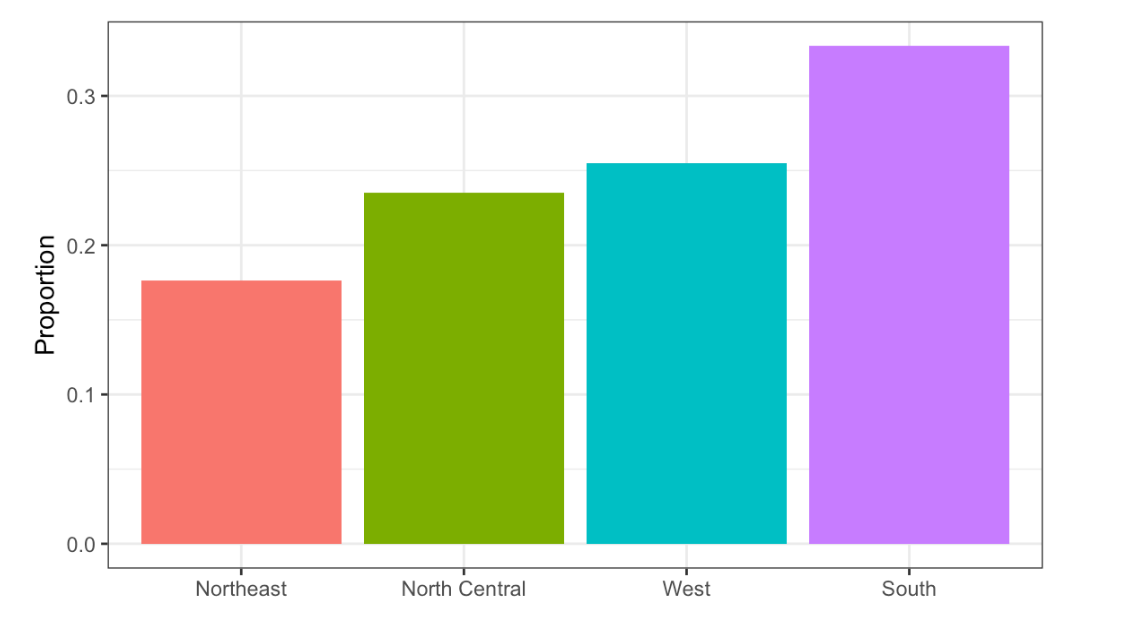
\includegraphics{images/Region vs Proportion.png}
\caption{Region vs.~Proportion}
\end{figure}

\begin{itemize}
\tightlist
\item[$\square$]
  A. 75\%
\item[$\square$]
  B. 50\%
\item[$\boxtimes$]
  C. 20\%
\item[$\square$]
  D. 5\%
\end{itemize}

\begin{enumerate}
\def\labelenumi{\arabic{enumi}.}
\setcounter{enumi}{1}
\tightlist
\item
  In the murders dataset, the region is a categorical variable and to
  the right is its distribution.
\end{enumerate}

Which of the following is true:

\begin{itemize}
\tightlist
\item[$\square$]
  A. The graph above is a histogram.
\item[$\boxtimes$]
  B. The graph above shows only four numbers with a bar plot.
\item[$\square$]
  C. Categories are not numbers, so it does not make sense to graph the
  distribution.
\item[$\square$]
  D. The colors, not the height of the bars, describe the distribution.
\end{itemize}

\begin{enumerate}
\def\labelenumi{\arabic{enumi}.}
\setcounter{enumi}{2}
\tightlist
\item
  The plot shows the eCDF for male heights.
\end{enumerate}

Based on the plot, what percentage of males are shorter than 75 inches?

\begin{figure}
\centering
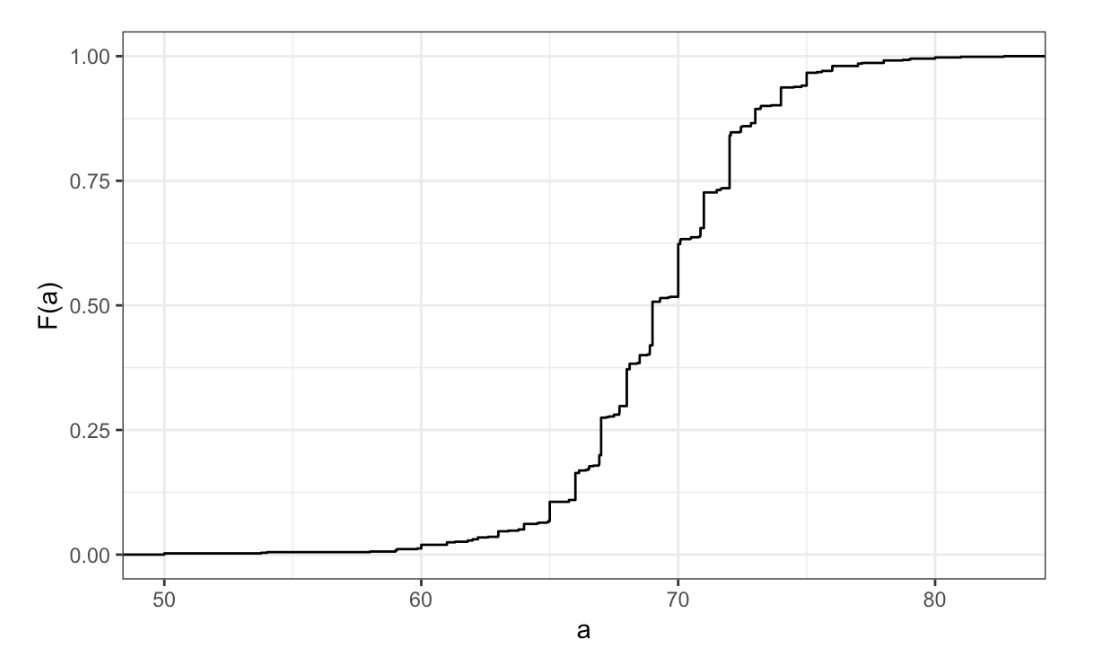
\includegraphics{images/eCDF for male heights.png}
\caption{eCDF for male heights}
\end{figure}

\begin{itemize}
\tightlist
\item[$\square$]
  A. 100\%
\item[$\boxtimes$]
  B. 95\%
\item[$\square$]
  C. 80\%
\item[$\square$]
  D. 72 inches
\end{itemize}

\begin{enumerate}
\def\labelenumi{\arabic{enumi}.}
\setcounter{enumi}{3}
\tightlist
\item
  To the closest inch, what height \texttt{m} has the property that 1/2
  of the male students are taller than \texttt{m} and 1/2 are shorter?
\end{enumerate}

\begin{itemize}
\tightlist
\item[$\square$]
  A. 61 inches
\item[$\square$]
  B. 64 inches
\item[$\boxtimes$]
  C. 69 inches
\item[$\square$]
  D. 74 inches
\end{itemize}

\newpage

\begin{enumerate}
\def\labelenumi{\arabic{enumi}.}
\setcounter{enumi}{4}
\tightlist
\item
  Here is an eCDF of the murder rates across states.
\end{enumerate}

\begin{figure}
\centering
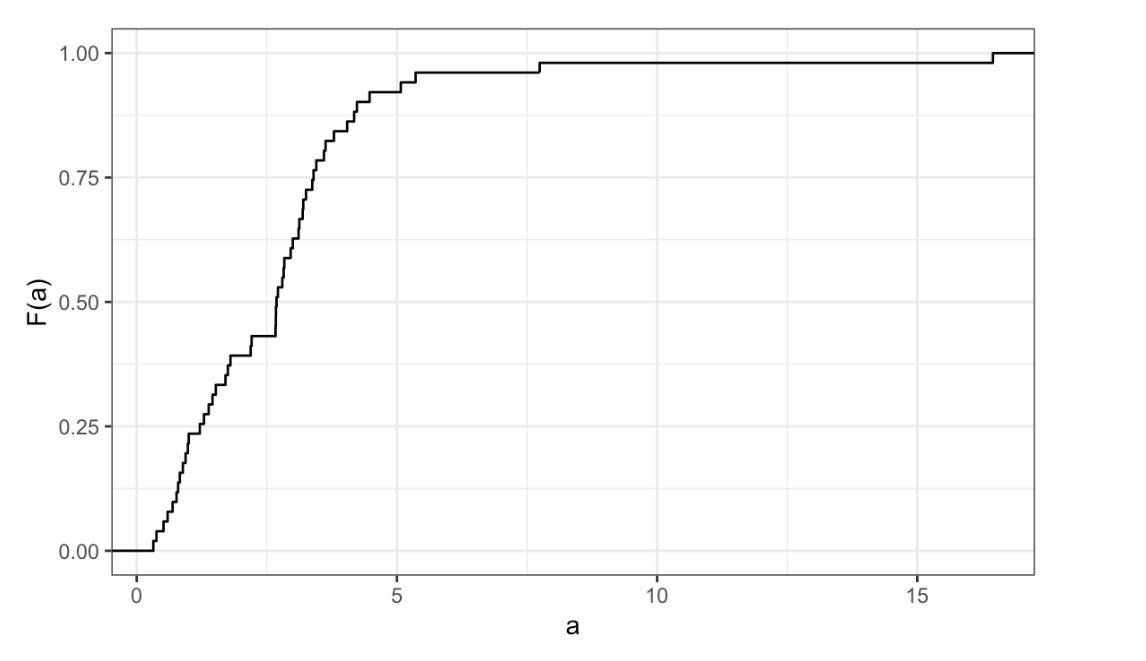
\includegraphics{images/eCDF murder rates across states.png}
\caption{eCDF of the murder rates across states}
\end{figure}

Knowing that there are 51 states (counting DC) and based on this plot,
how many states have murder rates larger than 10 per 100,000 people?

\begin{itemize}
\tightlist
\item[$\boxtimes$]
  A. 1
\item[$\square$]
  B. 5
\item[$\square$]
  C. 10
\item[$\square$]
  D. 50
\end{itemize}

\begin{enumerate}
\def\labelenumi{\arabic{enumi}.}
\setcounter{enumi}{5}
\tightlist
\item
  Based on the eCDF above, which of the following statements are true.
\end{enumerate}

\begin{itemize}
\tightlist
\item[$\square$]
  A. About half the states have murder rates above 7 per 100,000 and the
  other half below.
\item[$\square$]
  B. Most states have murder rates below 2 per 100,000.
\item[$\square$]
  C. All the states have murder rates above 2 per 100,000.
\item[$\boxtimes$]
  D. With the exception of 4 states, the murder rates are below 5 per
  100,000.
\end{itemize}

\newpage

\begin{enumerate}
\def\labelenumi{\arabic{enumi}.}
\setcounter{enumi}{6}
\tightlist
\item
  Here is a histogram of male heights in our \texttt{heights} dataset.
\end{enumerate}

Based on this plot, how many males are between 62.5 and 65.5?

\begin{figure}
\centering
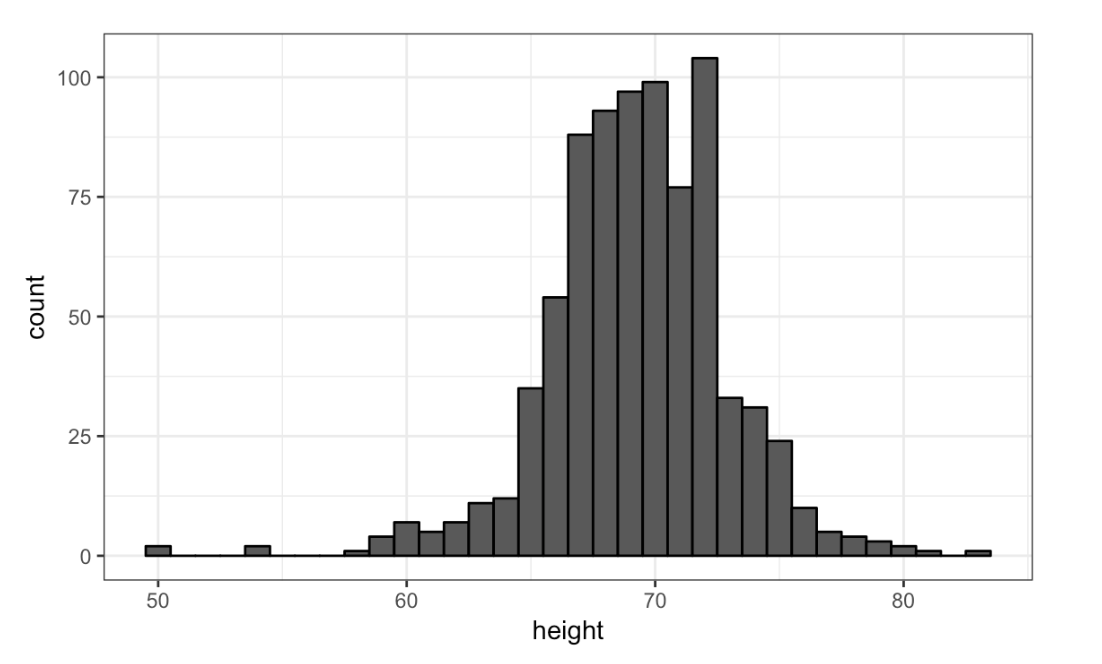
\includegraphics{images/Histogram of male heights.png}
\caption{Histogram of male heights}
\end{figure}

\begin{itemize}
\tightlist
\item[$\square$]
  A. 11
\item[$\square$]
  B. 29
\item[$\boxtimes$]
  C. 58
\item[$\square$]
  D. 99
\end{itemize}

\begin{enumerate}
\def\labelenumi{\arabic{enumi}.}
\setcounter{enumi}{7}
\tightlist
\item
  About what percentage are shorter than 60 inches?
\end{enumerate}

\begin{itemize}
\tightlist
\item[$\boxtimes$]
  A. 1\%
\item[$\square$]
  B. 10\%
\item[$\square$]
  C. 25\%
\item[$\square$]
  D. 50\%
\end{itemize}

\newpage

\begin{enumerate}
\def\labelenumi{\arabic{enumi}.}
\setcounter{enumi}{8}
\tightlist
\item
  Based on this density plot, about what proportion of US states have
  populations larger than 10 million?
\end{enumerate}

\begin{figure}
\centering
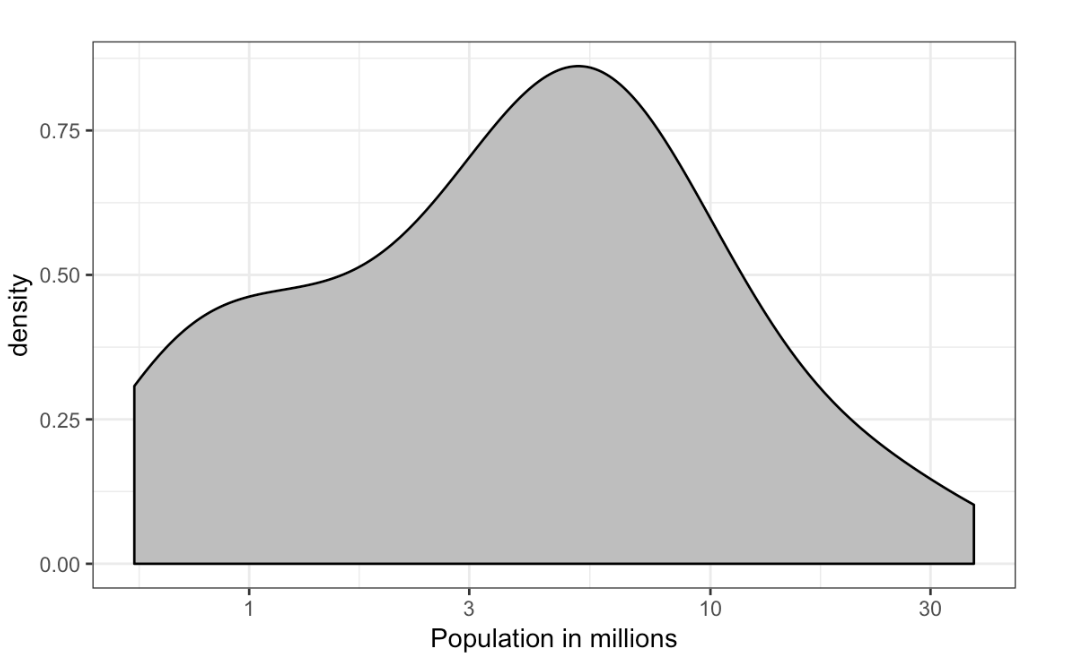
\includegraphics{images/Density plot population.png}
\caption{Density plot population}
\end{figure}

\begin{itemize}
\tightlist
\item[$\square$]
  A. 0.02
\item[$\boxtimes$]
  B. 0.15
\item[$\square$]
  C. 0.50
\item[$\square$]
  D. 0.55
\end{itemize}

\begin{enumerate}
\def\labelenumi{\arabic{enumi}.}
\setcounter{enumi}{9}
\tightlist
\item
  Below are three density plots. Is it possible that they are from the
  same dataset?
\end{enumerate}

\begin{figure}
\centering
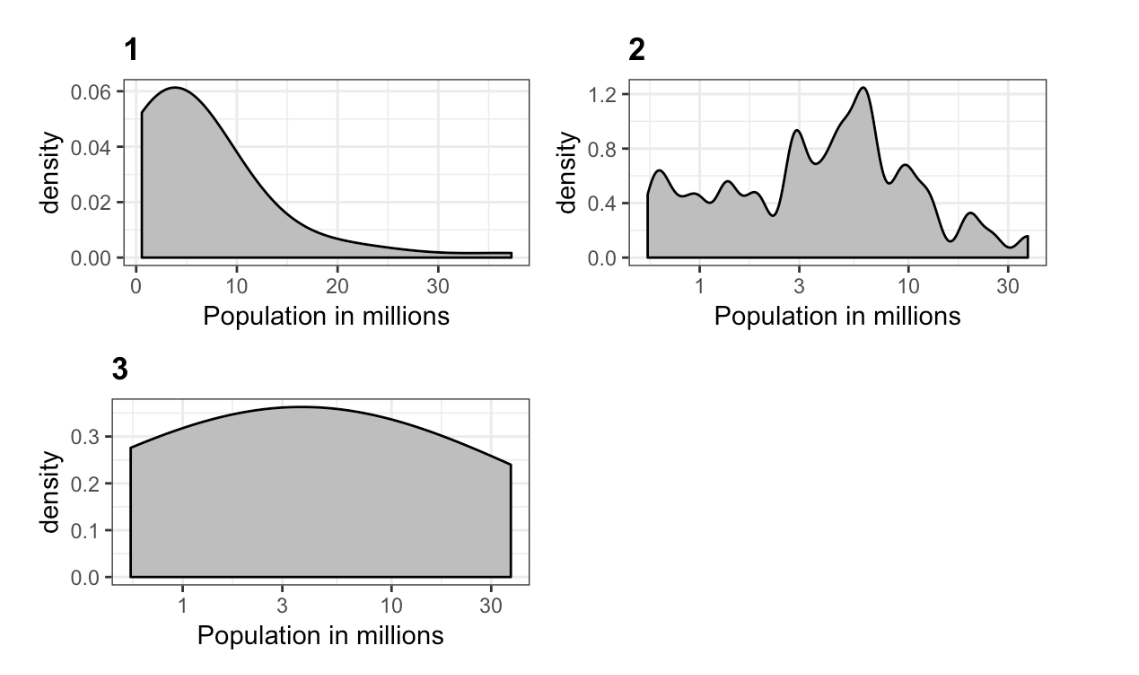
\includegraphics{images/Three density plots.png}
\caption{Three density plots}
\end{figure}

Which of the following statements is true?

\begin{itemize}
\tightlist
\item[$\square$]
  A. It is impossible that they are from the same dataset.
\item[$\square$]
  B. They are from the same dataset, but the plots are different due to
  code errors.
\item[$\square$]
  C. They are the same dataset, but the first and second plot
  undersmooth and the third oversmooths.
\item[$\boxtimes$]
  D. They are the same dataset, but the first is not in the log scale,
  the second undersmooths and the third oversmooths.
\end{itemize}

\newpage

\hypertarget{normal-distribution}{%
\subsection{Normal Distribution}\label{normal-distribution}}

The textbook for this section is available
\href{https://rafalab.github.io/dsbook/distributions.html\#normal-distribution}{here}

\textbf{Key points}

\begin{itemize}
\item
  The normal distribution:

  \begin{itemize}
  \tightlist
  \item
    Is centered around one value, the \emph{mean}
  \item
    Is symmetric around the mean
  \item
    Is defined completely by its mean (\(\mu\)) and standard deviation
    (\(\sigma\))
  \item
    Always has the same proportion of observations within a given
    distance of the mean (for example, 95\% within 2 \(\sigma\))
  \end{itemize}
\item
  The standard deviation is the average distance between a value and the
  mean value.
\item
  Calculate the mean using the \texttt{mean} function.
\item
  Calculate the standard deviation using the \texttt{sd} function or
  manually.
\item
  Standard units describe how many standard deviations a value is away
  from the mean. The z-score, or number of standard deviations an
  observation \emph{x} is away from the mean (\(\mu\)):

  \(Z = \frac{x - \mu}{\sigma}\)
\item
  Compute standard units with the \texttt{scale} function.
\item
  \textbf{Important:} to calculate the proportion of values that meet a
  certain condition, use the \texttt{mean} function on a logical vector.
  Because TRUE is converted to 1 and FALSE is converted to 0, taking the
  mean of this vector yields the proportion of TRUE.
\end{itemize}

\textbf{Equation for the normal distribution}

The normal distribution is mathematically defined by the following
formula for any mean \(\mu\) and standard deviation \(\sigma\):

\(Pr(a < x < b) = \int_{a}^{b} \frac{1}{\sqrt2\pi\sigma} e^-\frac{1}{2}(\frac{x - \mu}{\sigma})^2 dx\)

\emph{Code}

\begin{Shaded}
\begin{Highlighting}[]
\CommentTok{# define x as vector of male heights}
\KeywordTok{library}\NormalTok{(tidyverse)}
\end{Highlighting}
\end{Shaded}

\begin{verbatim}
## -- Attaching packages --------------------------------------------------------------------------------------------------------------------------------------------- tidyverse 1.3.0 --
\end{verbatim}

\begin{verbatim}
## v ggplot2 3.3.2     v purrr   0.3.4
## v tibble  3.0.3     v dplyr   1.0.0
## v tidyr   1.1.0     v stringr 1.4.0
## v readr   1.3.1     v forcats 0.5.0
\end{verbatim}

\begin{verbatim}
## -- Conflicts ------------------------------------------------------------------------------------------------------------------------------------------------ tidyverse_conflicts() --
## x dplyr::filter() masks stats::filter()
## x dplyr::lag()    masks stats::lag()
\end{verbatim}

\begin{Shaded}
\begin{Highlighting}[]
\NormalTok{index <-}\StringTok{ }\NormalTok{heights}\OperatorTok{$}\NormalTok{sex}\OperatorTok{==}\StringTok{"Male"}
\NormalTok{x <-}\StringTok{ }\NormalTok{heights}\OperatorTok{$}\NormalTok{height[index]}

\CommentTok{# calculate the mean and standard deviation manually}
\NormalTok{average <-}\StringTok{ }\KeywordTok{sum}\NormalTok{(x)}\OperatorTok{/}\KeywordTok{length}\NormalTok{(x)}
\NormalTok{SD <-}\StringTok{ }\KeywordTok{sqrt}\NormalTok{(}\KeywordTok{sum}\NormalTok{((x }\OperatorTok{-}\StringTok{ }\NormalTok{average)}\OperatorTok{^}\DecValTok{2}\NormalTok{)}\OperatorTok{/}\KeywordTok{length}\NormalTok{(x))}

\CommentTok{# built-in mean and sd functions - note that the audio and printed values disagree}
\NormalTok{average <-}\StringTok{ }\KeywordTok{mean}\NormalTok{(x)}
\NormalTok{SD <-}\StringTok{ }\KeywordTok{sd}\NormalTok{(x)}
\KeywordTok{c}\NormalTok{(}\DataTypeTok{average =}\NormalTok{ average, }\DataTypeTok{SD =}\NormalTok{ SD)}
\end{Highlighting}
\end{Shaded}

\begin{verbatim}
##   average        SD 
## 69.314755  3.611024
\end{verbatim}

\begin{Shaded}
\begin{Highlighting}[]
\CommentTok{# calculate standard units}
\NormalTok{z <-}\StringTok{ }\KeywordTok{scale}\NormalTok{(x)}

\CommentTok{# calculate proportion of values within 2 SD of mean}
\KeywordTok{mean}\NormalTok{(}\KeywordTok{abs}\NormalTok{(z) }\OperatorTok{<}\StringTok{ }\DecValTok{2}\NormalTok{)}
\end{Highlighting}
\end{Shaded}

\begin{verbatim}
## [1] 0.9495074
\end{verbatim}

\textbf{Note about the sd function:} The built-in R function \texttt{sd}
calculates the standard deviation, but it divides by
\texttt{length(x)-1} instead of \texttt{length(x)}. When the length of
the list is large, this difference is negligible and you can use the
built-in \texttt{sd} function. Otherwise, you should compute \(\sigma\)
by hand. For this course series, assume that you should use the
\texttt{sd} function unless you are told not to do so.

\hypertarget{assessment---normal-distribution}{%
\subsection{Assessment - Normal
Distribution}\label{assessment---normal-distribution}}

\begin{enumerate}
\def\labelenumi{\arabic{enumi}.}
\tightlist
\item
  Histograms and density plots provide excellent summaries of a
  distribution.
\end{enumerate}

But can we summarize even further? We often see the average and standard
deviation used as summary statistics: a two number summary! To
understand what these summaries are and why they are so widely used, we
need to understand the normal distribution.

The normal distribution, also known as the bell curve and as the
Gaussian distribution, is one of the most famous mathematical concepts
in history. A reason for this is that approximately normal distributions
occur in many situations. Examples include gambling winnings, heights,
weights, blood pressure, standardized test scores, and experimental
measurement errors. Often data visualization is needed to confirm that
our data follows a normal distribution.

Here we focus on how the normal distribution helps us summarize data and
can be useful in practice.

One way the normal distribution is useful is that it can be used to
approximate the distribution of a list of numbers without having access
to the entire list. We will demonstrate this with the heights dataset.

Load the height data set and create a vector \texttt{x} with just the
male heights:

\begin{Shaded}
\begin{Highlighting}[]
\KeywordTok{library}\NormalTok{(dslabs)}
\KeywordTok{data}\NormalTok{(heights)}
\NormalTok{x <-}\StringTok{ }\NormalTok{heights}\OperatorTok{$}\NormalTok{height[heights}\OperatorTok{$}\NormalTok{sex }\OperatorTok{==}\StringTok{ "Male"}\NormalTok{]}
\end{Highlighting}
\end{Shaded}

What proportion of the data is between 69 and 72 inches (taller than 69
but shorter or equal to 72)? A proportion is between 0 and 1.

\begin{Shaded}
\begin{Highlighting}[]
\NormalTok{x <-}\StringTok{ }\NormalTok{heights}\OperatorTok{$}\NormalTok{height[heights}\OperatorTok{$}\NormalTok{sex }\OperatorTok{==}\StringTok{ "Male"}\NormalTok{]}
\KeywordTok{mean}\NormalTok{(x }\OperatorTok{>}\StringTok{ }\DecValTok{69} \OperatorTok{&}\StringTok{ }\NormalTok{x }\OperatorTok{<=}\StringTok{ }\DecValTok{72}\NormalTok{)}
\end{Highlighting}
\end{Shaded}

\begin{verbatim}
## [1] 0.3337438
\end{verbatim}

\begin{enumerate}
\def\labelenumi{\arabic{enumi}.}
\setcounter{enumi}{1}
\tightlist
\item
  Suppose all you know about the height data from the previous exercise
  is the average and the standard deviation and that its distribution is
  approximated by the normal distribution.
\end{enumerate}

We can compute the average and standard deviation like this:

\begin{Shaded}
\begin{Highlighting}[]
\KeywordTok{library}\NormalTok{(dslabs)}
\KeywordTok{data}\NormalTok{(heights)}
\NormalTok{x <-}\StringTok{ }\NormalTok{heights}\OperatorTok{$}\NormalTok{height[heights}\OperatorTok{$}\NormalTok{sex}\OperatorTok{==}\StringTok{"Male"}\NormalTok{]}
\NormalTok{avg <-}\StringTok{ }\KeywordTok{mean}\NormalTok{(x)}
\NormalTok{stdev <-}\StringTok{ }\KeywordTok{sd}\NormalTok{(x)}
\end{Highlighting}
\end{Shaded}

Suppose you only have \texttt{avg} and \texttt{stdev} below, but no
access to \texttt{x}, can you approximate the proportion of the data
that is between 69 and 72 inches?

Given a normal distribution with a mean \texttt{mu} and standard
deviation \texttt{sigma}, you can calculate the proportion of
observations less than or equal to a certain \texttt{value} with
\texttt{pnorm(value,\ mu,\ sigma)}. Notice that this is the CDF for the
normal distribution. We will learn much more about \texttt{pnorm} later
in the course series, but you can also learn more now with
\texttt{?pnorm}.

\begin{Shaded}
\begin{Highlighting}[]
\NormalTok{x <-}\StringTok{ }\NormalTok{heights}\OperatorTok{$}\NormalTok{height[heights}\OperatorTok{$}\NormalTok{sex}\OperatorTok{==}\StringTok{"Male"}\NormalTok{]}
\NormalTok{avg <-}\StringTok{ }\KeywordTok{mean}\NormalTok{(x)}
\NormalTok{stdev <-}\StringTok{ }\KeywordTok{sd}\NormalTok{(x)}
\KeywordTok{pnorm}\NormalTok{(}\DecValTok{72}\NormalTok{, avg, stdev) }\OperatorTok{-}\StringTok{ }\KeywordTok{pnorm}\NormalTok{(}\DecValTok{69}\NormalTok{, avg, stdev)}
\end{Highlighting}
\end{Shaded}

\begin{verbatim}
## [1] 0.3061779
\end{verbatim}

\begin{enumerate}
\def\labelenumi{\arabic{enumi}.}
\setcounter{enumi}{2}
\tightlist
\item
  Notice that the approximation calculated in the second question is
  very close to the exact calculation in the first question.
\end{enumerate}

The normal distribution was a useful approximation for this case.
However, the approximation is not always useful. An example is for the
more extreme values, often called the ``tails'' of the distribution.
Let's look at an example. We can compute the proportion of heights
between 79 and 81.

\begin{Shaded}
\begin{Highlighting}[]
\KeywordTok{library}\NormalTok{(dslabs)  }
\KeywordTok{data}\NormalTok{(heights)}
\NormalTok{x <-}\StringTok{ }\NormalTok{heights}\OperatorTok{$}\NormalTok{height[heights}\OperatorTok{$}\NormalTok{sex }\OperatorTok{==}\StringTok{ "Male"}\NormalTok{]  }
\KeywordTok{mean}\NormalTok{(x }\OperatorTok{>}\StringTok{ }\DecValTok{79} \OperatorTok{&}\StringTok{ }\NormalTok{x }\OperatorTok{<=}\StringTok{ }\DecValTok{81}\NormalTok{)  }
\end{Highlighting}
\end{Shaded}

\begin{Shaded}
\begin{Highlighting}[]
\NormalTok{x <-}\StringTok{ }\NormalTok{heights}\OperatorTok{$}\NormalTok{height[heights}\OperatorTok{$}\NormalTok{sex }\OperatorTok{==}\StringTok{ "Male"}\NormalTok{]}
\NormalTok{avg <-}\StringTok{ }\KeywordTok{mean}\NormalTok{(x)}
\NormalTok{stdev <-}\StringTok{ }\KeywordTok{sd}\NormalTok{(x)}
\NormalTok{exact <-}\StringTok{ }\KeywordTok{mean}\NormalTok{(x }\OperatorTok{>}\StringTok{ }\DecValTok{79} \OperatorTok{&}\StringTok{ }\NormalTok{x }\OperatorTok{<=}\StringTok{ }\DecValTok{81}\NormalTok{)}
\NormalTok{approx <-}\StringTok{ }\KeywordTok{pnorm}\NormalTok{(}\DecValTok{81}\NormalTok{, avg, stdev) }\OperatorTok{-}\StringTok{ }\KeywordTok{pnorm}\NormalTok{(}\DecValTok{79}\NormalTok{, avg, stdev)}
\NormalTok{exact}
\end{Highlighting}
\end{Shaded}

\begin{verbatim}
## [1] 0.004926108
\end{verbatim}

\begin{Shaded}
\begin{Highlighting}[]
\NormalTok{approx}
\end{Highlighting}
\end{Shaded}

\begin{verbatim}
## [1] 0.003051617
\end{verbatim}

\begin{Shaded}
\begin{Highlighting}[]
\NormalTok{exact}\OperatorTok{/}\NormalTok{approx}
\end{Highlighting}
\end{Shaded}

\begin{verbatim}
## [1] 1.614261
\end{verbatim}

\begin{enumerate}
\def\labelenumi{\arabic{enumi}.}
\setcounter{enumi}{3}
\tightlist
\item
  Someone asks you what percent of seven footers are in the National
  Basketball Association (NBA). Can you provide an estimate? Let's try
  using the normal approximation to answer this question.
\end{enumerate}

First, we will estimate the proportion of adult men that are 7 feet tall
or taller.

Assume that the distribution of adult men in the world as normally
distributed with an average of 69 inches and a standard deviation of 3
inches.

\begin{Shaded}
\begin{Highlighting}[]
\CommentTok{# use pnorm to calculate the proportion over 7 feet (7*12 inches)}
\DecValTok{1} \OperatorTok{-}\StringTok{ }\KeywordTok{pnorm}\NormalTok{(}\DecValTok{7}\OperatorTok{*}\DecValTok{12}\NormalTok{, }\DecValTok{69}\NormalTok{, }\DecValTok{3}\NormalTok{)}
\end{Highlighting}
\end{Shaded}

\begin{verbatim}
## [1] 2.866516e-07
\end{verbatim}

\begin{enumerate}
\def\labelenumi{\arabic{enumi}.}
\setcounter{enumi}{4}
\tightlist
\item
  Now we have an approximation for the proportion, call it \texttt{p},
  of men that are 7 feet tall or taller.
\end{enumerate}

We know that there are about 1 billion men between the ages of 18 and 40
in the world, the age range for the NBA.

Can we use the normal distribution to estimate how many of these 1
billion men are at least seven feet tall?

\begin{Shaded}
\begin{Highlighting}[]
\NormalTok{p <-}\StringTok{ }\DecValTok{1} \OperatorTok{-}\StringTok{ }\KeywordTok{pnorm}\NormalTok{(}\DecValTok{7}\OperatorTok{*}\DecValTok{12}\NormalTok{, }\DecValTok{69}\NormalTok{, }\DecValTok{3}\NormalTok{)}
\KeywordTok{round}\NormalTok{(p}\OperatorTok{*}\DecValTok{10}\OperatorTok{^}\DecValTok{9}\NormalTok{)}
\end{Highlighting}
\end{Shaded}

\begin{verbatim}
## [1] 287
\end{verbatim}

\begin{enumerate}
\def\labelenumi{\arabic{enumi}.}
\setcounter{enumi}{5}
\tightlist
\item
  There are about 10 National Basketball Association (NBA) players that
  are 7 feet tall or higher.
\end{enumerate}

\begin{Shaded}
\begin{Highlighting}[]
\NormalTok{p <-}\StringTok{ }\DecValTok{1} \OperatorTok{-}\StringTok{ }\KeywordTok{pnorm}\NormalTok{(}\DecValTok{7}\OperatorTok{*}\DecValTok{12}\NormalTok{, }\DecValTok{69}\NormalTok{, }\DecValTok{3}\NormalTok{)}
\NormalTok{N <-}\StringTok{ }\KeywordTok{round}\NormalTok{(p}\OperatorTok{*}\DecValTok{10}\OperatorTok{^}\DecValTok{9}\NormalTok{)}
\DecValTok{10}\OperatorTok{/}\NormalTok{N}
\end{Highlighting}
\end{Shaded}

\begin{verbatim}
## [1] 0.03484321
\end{verbatim}

\begin{enumerate}
\def\labelenumi{\arabic{enumi}.}
\setcounter{enumi}{6}
\tightlist
\item
  In the previous exerceise we estimated the proportion of seven footers
  in the NBA using this simple code:
\end{enumerate}

\begin{Shaded}
\begin{Highlighting}[]
\NormalTok{p <-}\StringTok{ }\DecValTok{1} \OperatorTok{-}\StringTok{ }\KeywordTok{pnorm}\NormalTok{(}\DecValTok{7}\OperatorTok{*}\DecValTok{12}\NormalTok{, }\DecValTok{69}\NormalTok{, }\DecValTok{3}\NormalTok{)  }
\NormalTok{N <-}\StringTok{ }\KeywordTok{round}\NormalTok{(p }\OperatorTok{*}\StringTok{ }\DecValTok{10}\OperatorTok{^}\DecValTok{9}\NormalTok{)  }
\DecValTok{10}\OperatorTok{/}\NormalTok{N  }
\end{Highlighting}
\end{Shaded}

Repeat the calculations performed in the previous question for Lebron
James' height: 6 feet 8 inches. There are about 150 players, instead of
10, that are at least that tall in the NBA.

\begin{Shaded}
\begin{Highlighting}[]
\CommentTok{## Change the solution to previous answer}
\NormalTok{p <-}\StringTok{ }\DecValTok{1} \OperatorTok{-}\StringTok{ }\KeywordTok{pnorm}\NormalTok{(}\DecValTok{7}\OperatorTok{*}\DecValTok{12}\NormalTok{, }\DecValTok{69}\NormalTok{, }\DecValTok{3}\NormalTok{)}
\NormalTok{N <-}\StringTok{ }\KeywordTok{round}\NormalTok{(p }\OperatorTok{*}\StringTok{ }\DecValTok{10}\OperatorTok{^}\DecValTok{9}\NormalTok{)}
\DecValTok{10}\OperatorTok{/}\NormalTok{N}
\end{Highlighting}
\end{Shaded}

\begin{verbatim}
## [1] 0.03484321
\end{verbatim}

\begin{Shaded}
\begin{Highlighting}[]
\NormalTok{p <-}\StringTok{ }\DecValTok{1} \OperatorTok{-}\StringTok{ }\KeywordTok{pnorm}\NormalTok{(}\DecValTok{6}\OperatorTok{*}\DecValTok{12}\OperatorTok{+}\DecValTok{8}\NormalTok{, }\DecValTok{69}\NormalTok{, }\DecValTok{3}\NormalTok{)}
\NormalTok{N <-}\StringTok{ }\KeywordTok{round}\NormalTok{(p }\OperatorTok{*}\StringTok{ }\DecValTok{10}\OperatorTok{^}\DecValTok{9}\NormalTok{)}
\DecValTok{150}\OperatorTok{/}\NormalTok{N}
\end{Highlighting}
\end{Shaded}

\begin{verbatim}
## [1] 0.001220842
\end{verbatim}

\begin{enumerate}
\def\labelenumi{\arabic{enumi}.}
\setcounter{enumi}{7}
\tightlist
\item
  In answering the previous questions, we found that it is not at all
  rare for a seven footer to become an NBA player.
\end{enumerate}

What would be a fair critique of our calculations?

\begin{itemize}
\tightlist
\item[$\square$]
  A. Practice and talent are what make a great basketball player, not
  height.
\item[$\square$]
  B. The normal approximation is not appropriate for heights.
\item[$\boxtimes$]
  C. As seen in exercise 3, the normal approximation tends to
  underestimate the extreme values. It's possible that there are more
  seven footers than we predicted.
\item[$\square$]
  D. As seen in exercise 3, the normal approximation tends to
  overestimate the extreme values. It's possible that there are less
  seven footers than we predicted.
\end{itemize}

\hypertarget{quantile-quantile-plots}{%
\subsection{Quantile-Quantile Plots}\label{quantile-quantile-plots}}

The textbook for this section is available
\href{https://rafalab.github.io/dsbook/distributions.html\#quantile-quantile-plots}{here}

\textbf{Key points}

\begin{itemize}
\tightlist
\item
  Quantile-quantile plots, or QQ-plots, are used to check whether
  distributions are well-approximated by a normal distribution.
\item
  Given a proportion \emph{p}, the quantile \emph{q} is the value such
  that the proportion of values in the data below \emph{q} is \emph{p}.
\item
  In a QQ-plot, the sample quantiles in the observed data are compared
  to the theoretical quantiles expected from the normal distribution. If
  the data are well-approximated by the normal distribution, then the
  points on the QQ-plot will fall near the identity line (sample =
  theoretical).
\item
  Calculate sample quantiles (observed quantiles) using the
  \texttt{quantile} function.
\item
  Calculate theoretical quantiles with the \texttt{qnorm} function.
  \texttt{qnorm} will calculate quantiles for the standard normal
  distribution (\(\mu = 0\), \(\sigma = 1\)) by default, but it can
  calculate quantiles for any normal distribution given mean and
  \texttt{sd} arguments. We will learn more about \texttt{qnorm} in the
  probability course.
\item
  Note that we will learn alternate ways to make QQ-plots with less code
  later in the series.
\end{itemize}

\emph{Code}

\begin{Shaded}
\begin{Highlighting}[]
\CommentTok{# define x and z}
\NormalTok{index <-}\StringTok{ }\NormalTok{heights}\OperatorTok{$}\NormalTok{sex}\OperatorTok{==}\StringTok{"Male"}
\NormalTok{x <-}\StringTok{ }\NormalTok{heights}\OperatorTok{$}\NormalTok{height[index]}
\NormalTok{z <-}\StringTok{ }\KeywordTok{scale}\NormalTok{(x)}

\CommentTok{# proportion of data below 69.5}
\KeywordTok{mean}\NormalTok{(x }\OperatorTok{<=}\StringTok{ }\FloatTok{69.5}\NormalTok{)}
\end{Highlighting}
\end{Shaded}

\begin{verbatim}
## [1] 0.5147783
\end{verbatim}

\begin{Shaded}
\begin{Highlighting}[]
\CommentTok{# calculate observed and theoretical quantiles}
\NormalTok{p <-}\StringTok{ }\KeywordTok{seq}\NormalTok{(}\FloatTok{0.05}\NormalTok{, }\FloatTok{0.95}\NormalTok{, }\FloatTok{0.05}\NormalTok{)}
\NormalTok{observed_quantiles <-}\StringTok{ }\KeywordTok{quantile}\NormalTok{(x, p)}
\NormalTok{theoretical_quantiles <-}\StringTok{ }\KeywordTok{qnorm}\NormalTok{(p, }\DataTypeTok{mean =} \KeywordTok{mean}\NormalTok{(x), }\DataTypeTok{sd =} \KeywordTok{sd}\NormalTok{(x))}

\CommentTok{# make QQ-plot}
\KeywordTok{plot}\NormalTok{(theoretical_quantiles, observed_quantiles)}
\KeywordTok{abline}\NormalTok{(}\DecValTok{0}\NormalTok{,}\DecValTok{1}\NormalTok{)}
\end{Highlighting}
\end{Shaded}

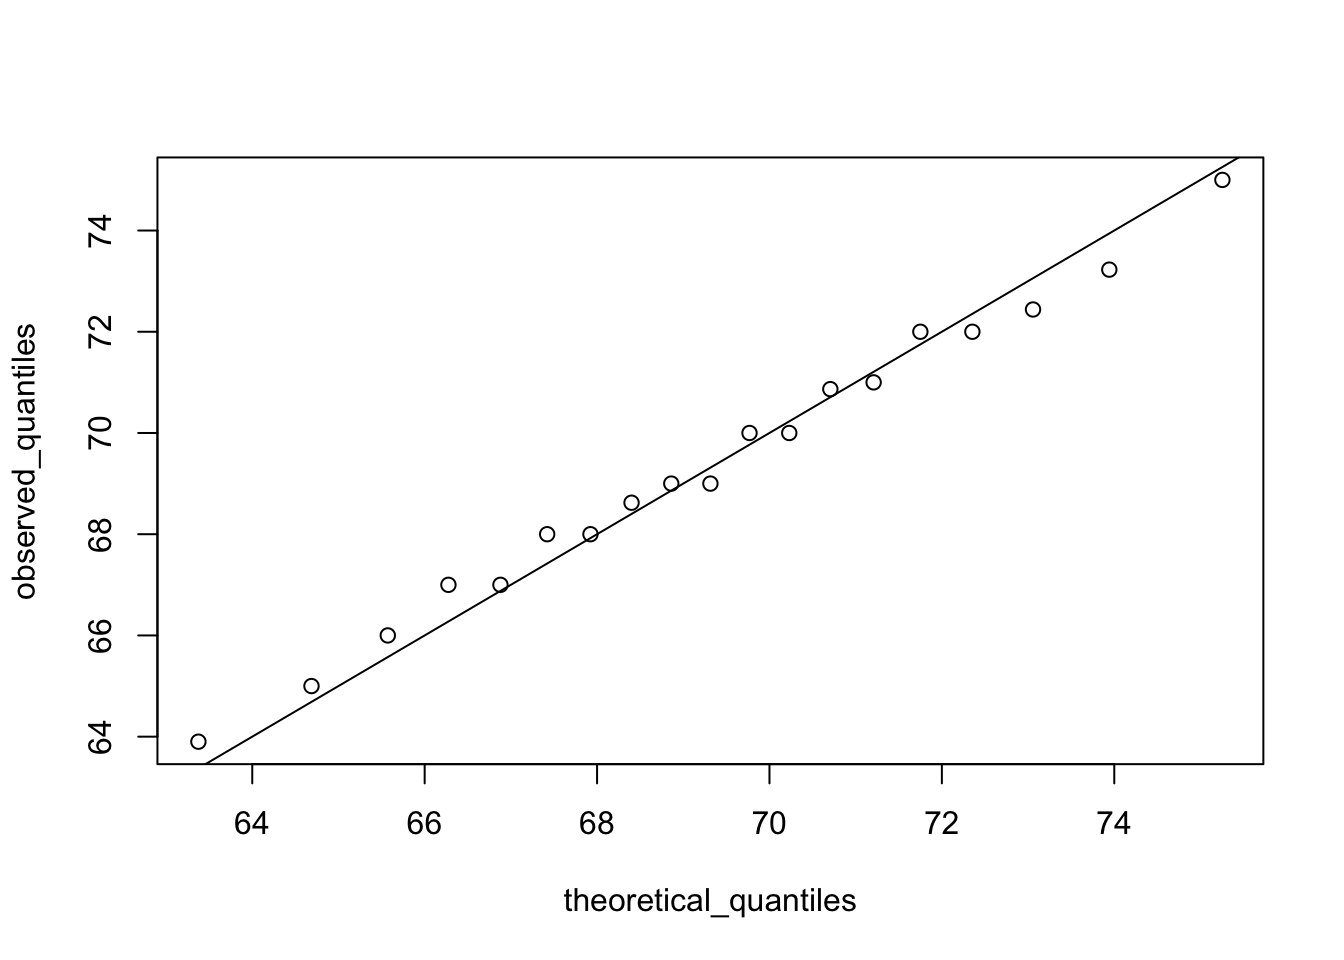
\includegraphics{Data_Science_Visualization_files/figure-latex/unnamed-chunk-24-1.pdf}

\begin{Shaded}
\begin{Highlighting}[]
\CommentTok{# make QQ-plot with scaled values}
\NormalTok{observed_quantiles <-}\StringTok{ }\KeywordTok{quantile}\NormalTok{(z, p)}
\NormalTok{theoretical_quantiles <-}\StringTok{ }\KeywordTok{qnorm}\NormalTok{(p) }
\KeywordTok{plot}\NormalTok{(theoretical_quantiles, observed_quantiles)}
\KeywordTok{abline}\NormalTok{(}\DecValTok{0}\NormalTok{,}\DecValTok{1}\NormalTok{)}
\end{Highlighting}
\end{Shaded}

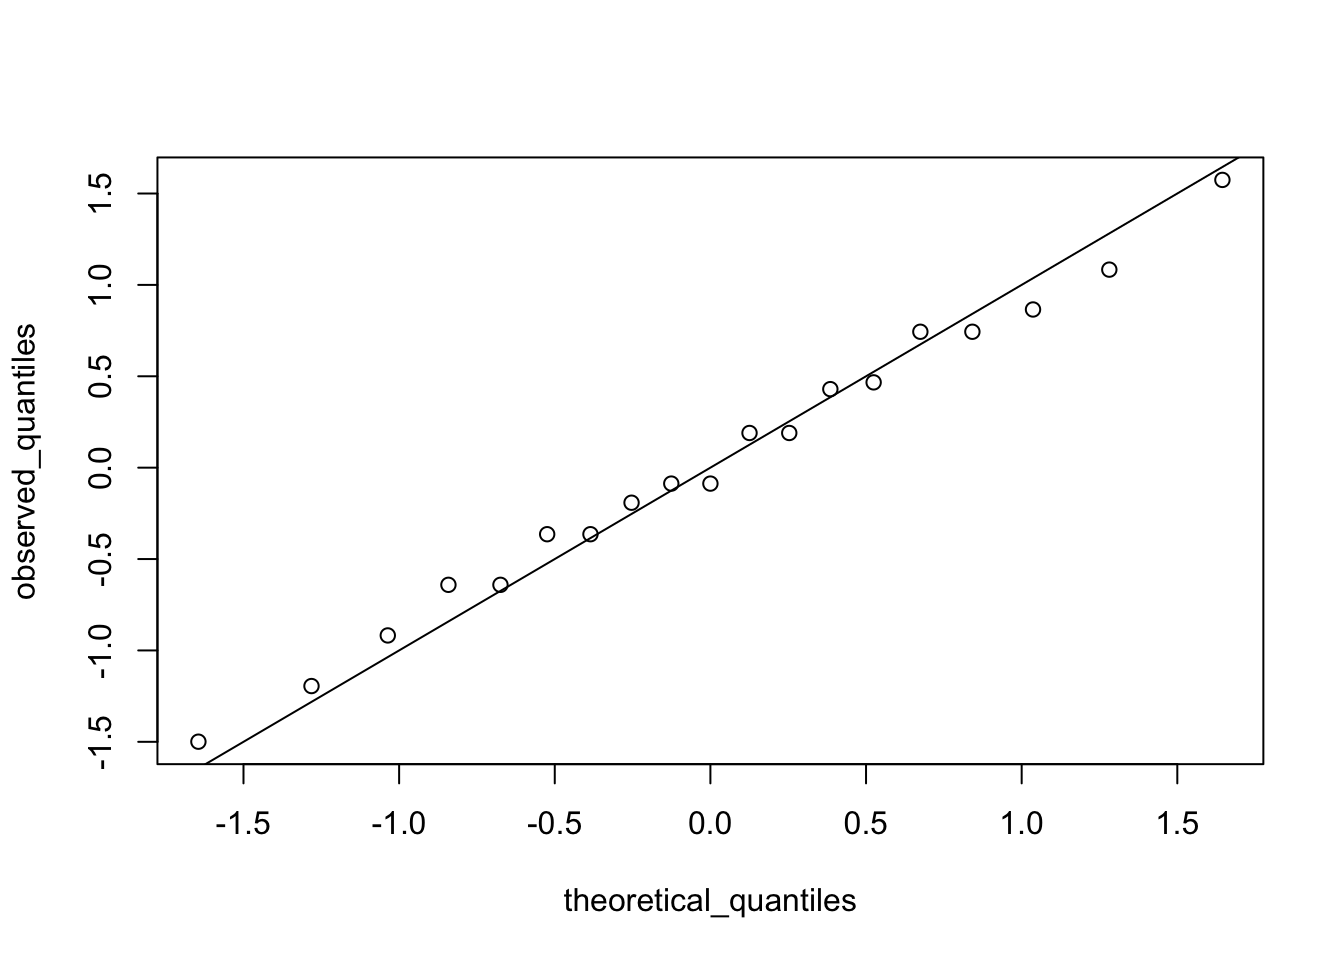
\includegraphics{Data_Science_Visualization_files/figure-latex/unnamed-chunk-24-2.pdf}

\hypertarget{percentiles}{%
\subsection{Percentiles}\label{percentiles}}

The textbook for this section is available
\href{https://rafalab.github.io/dsbook/distributions.html\#percentiles}{here}

\textbf{Key points}

\begin{itemize}
\tightlist
\item
  \emph{Percentiles} are the quantiles obtained when defining \emph{p}
  as \texttt{0.01,0.02,...,0.99}. They summarize the values at which a
  certain percent of the observations are equal to or less than that
  value.
\item
  The 50th percentile is also known as the \emph{median}.
\item
  The \emph{quartiles} are the 25th, 50th and 75th percentiles.
\end{itemize}

\hypertarget{boxplots}{%
\subsection{Boxplots}\label{boxplots}}

The textbook for this section is available
\href{https://rafalab.github.io/dsbook/distributions.html\#boxplots}{here}

\textbf{Key points}

\begin{itemize}
\tightlist
\item
  When data do not follow a normal distribution and cannot be succinctly
  summarized by only the mean and standard deviation, an alternative is
  to report a five-number summary: range (ignoring outliers) and the
  quartiles (25th, 50th, 75th percentile).
\item
  In a \emph{boxplot}, the box is defined by the 25th and 75th
  percentiles and the median is a horizontal line through the box. The
  whiskers show the range excluding outliers, and outliers are plotted
  separately as individual points.
\item
  The \emph{interquartile} range is the distance between the 25th and
  75th percentiles.
\item
  Boxplots are particularly useful when comparing multiple
  distributions.
\item
  We discuss outliers later.
\end{itemize}

\hypertarget{assessment---quantiles-percentiles-and-boxplots}{%
\subsection{Assessment - Quantiles, percentiles, and
boxplots}\label{assessment---quantiles-percentiles-and-boxplots}}

\begin{enumerate}
\def\labelenumi{\arabic{enumi}.}
\tightlist
\item
  When analyzing data it's often important to know the number of
  measurements you have for each category.
\end{enumerate}

\begin{Shaded}
\begin{Highlighting}[]
\NormalTok{male <-}\StringTok{ }\NormalTok{heights}\OperatorTok{$}\NormalTok{height[heights}\OperatorTok{$}\NormalTok{sex}\OperatorTok{==}\StringTok{"Male"}\NormalTok{]}
\NormalTok{female <-}\StringTok{ }\NormalTok{heights}\OperatorTok{$}\NormalTok{height[heights}\OperatorTok{$}\NormalTok{sex}\OperatorTok{==}\StringTok{"Female"}\NormalTok{]}
\KeywordTok{length}\NormalTok{(male)}
\end{Highlighting}
\end{Shaded}

\begin{verbatim}
## [1] 812
\end{verbatim}

\begin{Shaded}
\begin{Highlighting}[]
\KeywordTok{length}\NormalTok{(female)}
\end{Highlighting}
\end{Shaded}

\begin{verbatim}
## [1] 238
\end{verbatim}

\begin{enumerate}
\def\labelenumi{\arabic{enumi}.}
\setcounter{enumi}{1}
\tightlist
\item
  Suppose we can't make a plot and want to compare the distributions
  side by side. If the number of data points is large, listing all the
  numbers is inpractical. A more practical approach is to look at the
  percentiles. We can obtain percentiles using the \texttt{quantile}
  function like this
\end{enumerate}

\begin{Shaded}
\begin{Highlighting}[]
\KeywordTok{library}\NormalTok{(dslabs)}
\KeywordTok{data}\NormalTok{(heights)}
\KeywordTok{quantile}\NormalTok{(heights}\OperatorTok{$}\NormalTok{height, }\KeywordTok{seq}\NormalTok{(.}\DecValTok{01}\NormalTok{, }\FloatTok{0.99}\NormalTok{, }\FloatTok{0.01}\NormalTok{))}
\end{Highlighting}
\end{Shaded}

\begin{Shaded}
\begin{Highlighting}[]
\NormalTok{male <-}\StringTok{ }\NormalTok{heights}\OperatorTok{$}\NormalTok{height[heights}\OperatorTok{$}\NormalTok{sex}\OperatorTok{==}\StringTok{"Male"}\NormalTok{]}
\NormalTok{female <-}\StringTok{ }\NormalTok{heights}\OperatorTok{$}\NormalTok{height[heights}\OperatorTok{$}\NormalTok{sex}\OperatorTok{==}\StringTok{"Female"}\NormalTok{]}
\NormalTok{female_percentiles <-}\StringTok{ }\KeywordTok{quantile}\NormalTok{(female, }\KeywordTok{seq}\NormalTok{(}\FloatTok{0.1}\NormalTok{, }\FloatTok{0.9}\NormalTok{, }\FloatTok{0.2}\NormalTok{))}
\NormalTok{male_percentiles <-}\StringTok{ }\KeywordTok{quantile}\NormalTok{(male, }\KeywordTok{seq}\NormalTok{(}\FloatTok{0.1}\NormalTok{, }\FloatTok{0.9}\NormalTok{, }\FloatTok{0.2}\NormalTok{))}
\NormalTok{df <-}\StringTok{ }\KeywordTok{data.frame}\NormalTok{(}\DataTypeTok{female =}\NormalTok{ (female_percentiles), }\DataTypeTok{male =}\NormalTok{ (male_percentiles))}
\NormalTok{df}
\end{Highlighting}
\end{Shaded}

\begin{verbatim}
##       female     male
## 10% 61.00000 65.00000
## 30% 63.00000 68.00000
## 50% 64.98031 69.00000
## 70% 66.46417 71.00000
## 90% 69.00000 73.22751
\end{verbatim}

\begin{enumerate}
\def\labelenumi{\arabic{enumi}.}
\setcounter{enumi}{2}
\tightlist
\item
  Study the boxplots summarizing the distributions of populations sizes
  by country.
\end{enumerate}

\begin{figure}
\centering
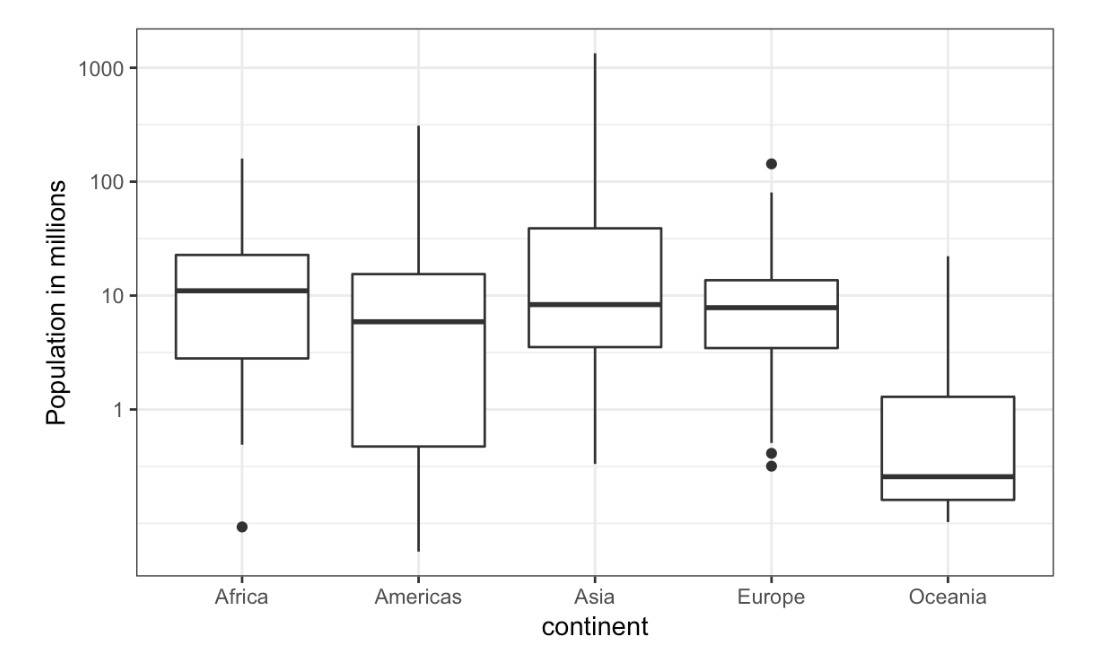
\includegraphics{images/Continent vs Population.png}
\caption{Continent vs Population}
\end{figure}

Which continent has the country with the largest population size?

\begin{itemize}
\tightlist
\item[$\square$]
  A. Africa
\item[$\square$]
  B. Americas
\item[$\boxtimes$]
  C. Asia
\item[$\square$]
  D. Europe
\item[$\square$]
  E. Oceania
\end{itemize}

\begin{enumerate}
\def\labelenumi{\arabic{enumi}.}
\setcounter{enumi}{3}
\tightlist
\item
  Study the boxplots summarizing the distributions of populations sizes
  by country.
\end{enumerate}

Which continent has median country with the largest population?

\begin{itemize}
\tightlist
\item[$\boxtimes$]
  A. Africa
\item[$\square$]
  B. Americas
\item[$\square$]
  C. Asia
\item[$\square$]
  D. Europe
\item[$\square$]
  E. Oceania
\end{itemize}

\begin{enumerate}
\def\labelenumi{\arabic{enumi}.}
\setcounter{enumi}{4}
\tightlist
\item
  Again, look at the boxplots summarizing the distributions of
  populations sizes by country.
\end{enumerate}

To the nearest million, what is the median population size for Africa?

\begin{itemize}
\tightlist
\item[$\square$]
  A. 100 million
\item[$\square$]
  B. 25 million
\item[$\boxtimes$]
  C. 10 million
\item[$\square$]
  D. 5 million
\item[$\square$]
  E. 1 million
\end{itemize}

\begin{enumerate}
\def\labelenumi{\arabic{enumi}.}
\setcounter{enumi}{5}
\tightlist
\item
  Examine the following boxplots and report approximately what
  proportion of countries in Europe have populations below 14 million?
\end{enumerate}

\begin{itemize}
\tightlist
\item[$\boxtimes$]
  A. 0.75
\item[$\square$]
  B. 0.50
\item[$\square$]
  C. 0.25
\item[$\square$]
  D. 0.01
\end{itemize}

\begin{enumerate}
\def\labelenumi{\arabic{enumi}.}
\setcounter{enumi}{6}
\tightlist
\item
  Based on the boxplot, if we use a log transformation, which continent
  shown below has the largest interquartile range?
\end{enumerate}

\begin{itemize}
\tightlist
\item[$\square$]
  A. Africa
\item[$\boxtimes$]
  B. Americas
\item[$\square$]
  C. Asia
\item[$\square$]
  D. Europe
\item[$\square$]
  E. Oceania
\end{itemize}

\hypertarget{distribution-of-female-heights}{%
\subsection{Distribution of Female
Heights}\label{distribution-of-female-heights}}

The textbook for this section is available
\href{https://rafalab.github.io/dsbook/distributions.html\#student-height-cont}{here}

\textbf{Key points}

\begin{itemize}
\tightlist
\item
  If a distribution is not normal, it cannot be summarized with only the
  mean and standard deviation. Provide a histogram, smooth density or
  boxplot instead.
\item
  A plot can force us to see unexpected results that make us question
  the quality or implications of our data.
\end{itemize}

\hypertarget{assessment---robust-summaries-with-outliers}{%
\subsection{Assessment - Robust Summaries With
Outliers}\label{assessment---robust-summaries-with-outliers}}

\begin{enumerate}
\def\labelenumi{\arabic{enumi}.}
\tightlist
\item
  For this chapter, we will use height data collected by Francis Galton
  for his genetics studies. Here we just use height of the children in
  the dataset:
\end{enumerate}

\begin{Shaded}
\begin{Highlighting}[]
\KeywordTok{library}\NormalTok{(HistData)}
\KeywordTok{data}\NormalTok{(Galton)}
\NormalTok{x <-}\StringTok{ }\NormalTok{Galton}\OperatorTok{$}\NormalTok{child}
\end{Highlighting}
\end{Shaded}

\begin{Shaded}
\begin{Highlighting}[]
\KeywordTok{library}\NormalTok{(HistData)}
\end{Highlighting}
\end{Shaded}

\begin{verbatim}
## Warning: package 'HistData' was built under R version 4.0.2
\end{verbatim}

\begin{Shaded}
\begin{Highlighting}[]
\KeywordTok{data}\NormalTok{(Galton)}
\NormalTok{x <-}\StringTok{ }\NormalTok{Galton}\OperatorTok{$}\NormalTok{child}
\KeywordTok{mean}\NormalTok{(x)}
\end{Highlighting}
\end{Shaded}

\begin{verbatim}
## [1] 68.08847
\end{verbatim}

\begin{Shaded}
\begin{Highlighting}[]
\KeywordTok{median}\NormalTok{(x)}
\end{Highlighting}
\end{Shaded}

\begin{verbatim}
## [1] 68.2
\end{verbatim}

\begin{enumerate}
\def\labelenumi{\arabic{enumi}.}
\setcounter{enumi}{1}
\tightlist
\item
  Now for the same data compute the standard deviation and the median
  absolute deviation (MAD).
\end{enumerate}

\begin{Shaded}
\begin{Highlighting}[]
\NormalTok{x <-}\StringTok{ }\NormalTok{Galton}\OperatorTok{$}\NormalTok{child}
\KeywordTok{sd}\NormalTok{(x)}
\end{Highlighting}
\end{Shaded}

\begin{verbatim}
## [1] 2.517941
\end{verbatim}

\begin{Shaded}
\begin{Highlighting}[]
\KeywordTok{mad}\NormalTok{(x)}
\end{Highlighting}
\end{Shaded}

\begin{verbatim}
## [1] 2.9652
\end{verbatim}

\begin{enumerate}
\def\labelenumi{\arabic{enumi}.}
\setcounter{enumi}{2}
\tightlist
\item
  In the previous exercises we saw that the mean and median are very
  similar and so are the standard deviation and MAD. This is expected
  since the data is approximated by a normal distribution which has this
  property.
\end{enumerate}

Now suppose that suppose Galton made a mistake when entering the first
value, forgetting to use the decimal point. You can imitate this error
by typing:

\begin{Shaded}
\begin{Highlighting}[]
\KeywordTok{library}\NormalTok{(HistData)}
\KeywordTok{data}\NormalTok{(Galton)}
\NormalTok{x <-}\StringTok{ }\NormalTok{Galton}\OperatorTok{$}\NormalTok{child}
\NormalTok{x_with_error <-}\StringTok{ }\NormalTok{x}
\NormalTok{x_with_error[}\DecValTok{1}\NormalTok{] <-}\StringTok{ }\NormalTok{x_with_error[}\DecValTok{1}\NormalTok{]}\OperatorTok{*}\DecValTok{10}
\end{Highlighting}
\end{Shaded}

The data now has an outlier that the normal approximation does not
account for. Let's see how this affects the average.

\begin{Shaded}
\begin{Highlighting}[]
\NormalTok{x <-}\StringTok{ }\NormalTok{Galton}\OperatorTok{$}\NormalTok{child}
\NormalTok{x_with_error <-}\StringTok{ }\NormalTok{x}
\NormalTok{x_with_error[}\DecValTok{1}\NormalTok{] <-}\StringTok{ }\NormalTok{x_with_error[}\DecValTok{1}\NormalTok{]}\OperatorTok{*}\DecValTok{10}
\NormalTok{gem <-}\StringTok{ }\KeywordTok{mean}\NormalTok{(x)}
\NormalTok{gem_error <-}\StringTok{ }\KeywordTok{mean}\NormalTok{(x_with_error)}
\NormalTok{gem_error }\OperatorTok{-}\StringTok{ }\NormalTok{gem}
\end{Highlighting}
\end{Shaded}

\begin{verbatim}
## [1] 0.5983836
\end{verbatim}

\begin{enumerate}
\def\labelenumi{\arabic{enumi}.}
\setcounter{enumi}{3}
\tightlist
\item
  In the previous exercise we saw how a simple mistake in 1 out of over
  900 observations can result in the average of our data increasing more
  than half an inch, which is a large difference in practical terms.
\end{enumerate}

Now let's explore the effect this outlier has on the standard deviation.

\begin{Shaded}
\begin{Highlighting}[]
\NormalTok{x_with_error <-}\StringTok{ }\NormalTok{x}
\NormalTok{x_with_error[}\DecValTok{1}\NormalTok{] <-}\StringTok{ }\NormalTok{x_with_error[}\DecValTok{1}\NormalTok{]}\OperatorTok{*}\DecValTok{10}
\KeywordTok{sd}\NormalTok{(x_with_error)}\OperatorTok{-}\StringTok{ }\KeywordTok{sd}\NormalTok{(x)}
\end{Highlighting}
\end{Shaded}

\begin{verbatim}
## [1] 15.6746
\end{verbatim}

\begin{enumerate}
\def\labelenumi{\arabic{enumi}.}
\setcounter{enumi}{4}
\tightlist
\item
  In the previous exercises we saw how one mistake can have a
  substantial effect on the average and the standard deviation.
\end{enumerate}

Now we are going to see how the median and MAD are much more resistant
to outliers. For this reason we say that they are \emph{robust}
summaries.

\begin{Shaded}
\begin{Highlighting}[]
\NormalTok{x_with_error <-}\StringTok{ }\NormalTok{x}
\NormalTok{x_with_error[}\DecValTok{1}\NormalTok{] <-}\StringTok{ }\NormalTok{x_with_error[}\DecValTok{1}\NormalTok{]}\OperatorTok{*}\DecValTok{10}
\NormalTok{mediaan <-}\StringTok{ }\KeywordTok{median}\NormalTok{(x)}
\NormalTok{mediaan_error <-}\StringTok{ }\KeywordTok{median}\NormalTok{(x_with_error)}
\NormalTok{mediaan_error }\OperatorTok{-}\StringTok{ }\NormalTok{mediaan}
\end{Highlighting}
\end{Shaded}

\begin{verbatim}
## [1] 0
\end{verbatim}

\begin{enumerate}
\def\labelenumi{\arabic{enumi}.}
\setcounter{enumi}{5}
\tightlist
\item
  We saw that the median barely changes. Now let's see how the MAD is
  affected.
\end{enumerate}

We saw that the median barely changes. Now let's see how the MAD is
affected.

\begin{Shaded}
\begin{Highlighting}[]
\NormalTok{x_with_error <-}\StringTok{ }\NormalTok{x}
\NormalTok{x_with_error[}\DecValTok{1}\NormalTok{] <-}\StringTok{ }\NormalTok{x_with_error[}\DecValTok{1}\NormalTok{]}\OperatorTok{*}\DecValTok{10}
\NormalTok{mad_normal <-}\StringTok{ }\KeywordTok{mad}\NormalTok{(x)}
\NormalTok{mad_error <-}\StringTok{ }\KeywordTok{mad}\NormalTok{(x_with_error)}
\NormalTok{mad_error }\OperatorTok{-}\StringTok{ }\NormalTok{mad_normal}
\end{Highlighting}
\end{Shaded}

\begin{verbatim}
## [1] 0
\end{verbatim}

\begin{enumerate}
\def\labelenumi{\arabic{enumi}.}
\setcounter{enumi}{6}
\tightlist
\item
  How could you use exploratory data analysis to detect that an error
  was made?
\end{enumerate}

\begin{itemize}
\tightlist
\item[$\square$]
  A. Since it is only one value out of many, we will not be able to
  detect this.
\item[$\square$]
  B. We would see an obvious shift in the distribution.
\item[$\boxtimes$]
  C. A boxplot, histogram, or qq-plot would reveal a clear outlier.
\item[$\square$]
  D. A scatter plot would show high levels of measurement error.
\end{itemize}

\begin{enumerate}
\def\labelenumi{\arabic{enumi}.}
\setcounter{enumi}{7}
\tightlist
\item
  We have seen how the average can be affected by outliers.
\end{enumerate}

But how large can this effect get? This of course depends on the size of
the outlier and the size of the dataset.

To see how outliers can affect the average of a dataset, let's write a
simple function that takes the size of the outlier as input and returns
the average.

\begin{Shaded}
\begin{Highlighting}[]
\NormalTok{x <-}\StringTok{ }\NormalTok{Galton}\OperatorTok{$}\NormalTok{child}
\NormalTok{error_avg <-}\StringTok{ }\ControlFlowTok{function}\NormalTok{(k)\{}
\NormalTok{x[}\DecValTok{1}\NormalTok{] =}\StringTok{ }\NormalTok{k}
\KeywordTok{mean}\NormalTok{(x)}
\NormalTok{\}}
\KeywordTok{error_avg}\NormalTok{(}\DecValTok{10000}\NormalTok{)}
\end{Highlighting}
\end{Shaded}

\begin{verbatim}
## [1] 78.79784
\end{verbatim}

\begin{Shaded}
\begin{Highlighting}[]
\KeywordTok{error_avg}\NormalTok{(}\OperatorTok{-}\DecValTok{10000}\NormalTok{)}
\end{Highlighting}
\end{Shaded}

\begin{verbatim}
## [1] 57.24612
\end{verbatim}

\hypertarget{section-2-overview}{%
\subsection{Section 2 Overview}\label{section-2-overview}}

In Section 2, you will learn how to create data visualizations in R
using ggplot2.

After completing Section 2, you will:

\begin{itemize}
\tightlist
\item
  be able to use ggplot2 to create data visualizations in R.
\item
  be able to explain what the data component of a graph is.
\item
  be able to identify the geometry component of a graph and know when to
  use which type of geometry.
\item
  be able to explain what the aesthetic mapping component of a graph is.
\item
  be able to understand the scale component of a graph and select an
  appropriate scale component to use.
\end{itemize}

Note that it can be hard to memorize all of the functions and arguments
used by ggplot2, so we recommend that you have a
\href{https://rstudio.com/wp-content/uploads/2015/03/ggplot2-cheatsheet.pdf}{cheat
sheet} handy to help you remember the necessary commands.

\hypertarget{ggplot}{%
\subsection{ggplot}\label{ggplot}}

The textbook for this section is available
\href{https://rafalab.github.io/dsbook/ggplot2.html}{here}

\textbf{Key points}

\begin{itemize}
\tightlist
\item
  Throughout the series, we will create plots with the \textbf{ggplot2}
  package. ggplot2 is part of the tidyverse, which you can load with
  \texttt{library(tidyverse)}.
\item
  Note that you can also load ggplot2 alone using the command
  \texttt{library(ggplot2)}, instead of loading the entire tidyverse.
\item
  ggplot2 uses a \emph{grammar of graphics} to break plots into building
  blocks that have intuitive syntax, making it easy to create relatively
  complex and aesthetically pleasing plots with relatively simple and
  readable code.
\item
  ggplot2 is designed to work exclusively with tidy data (rows are
  observations and columns are variables).
\end{itemize}

\hypertarget{assessment-6-ggplot2}{%
\subsection{Assessment 6 (ggplot2)}\label{assessment-6-ggplot2}}

Start by loading the dplyr and ggplot2 library as well as the murders
and heights data.

\begin{verbatim}
library(dplyr)
library(ggplot2)
library(dslabs)
data(heights)
data(murders)
\end{verbatim}

\begin{enumerate}
\def\labelenumi{\arabic{enumi}.}
\tightlist
\item
  ggplot2 basics
\end{enumerate}

With ggplot2 plots can be saved as objects. For example we can associate
a dataset with a plot object like this

\begin{verbatim}
p <- ggplot(data = murders)
\end{verbatim}

Because data is the first argument we don't need to spell it out

\begin{verbatim}
p <- ggplot(murders)
\end{verbatim}

or, if we load dplyr, we can also use the pipe:

\begin{verbatim}
p <- murders %>% ggplot()
\end{verbatim}

Remember the pipe sends the object on the left of \%\textgreater\% to be
the first argument for the function the right of \%\textgreater\%. What
is class of the object p?

\begin{verbatim}
class(p)
\end{verbatim}

\begin{verbatim}
## [1] "gg"     "ggplot"
\end{verbatim}

\begin{enumerate}
\def\labelenumi{\arabic{enumi}.}
\setcounter{enumi}{1}
\tightlist
\item
  Printing
\end{enumerate}

Remember that to print an object you can use the command print or simply
type the object. For example

\begin{verbatim}
x <- 2
x
\end{verbatim}

\begin{verbatim}
## [1] 2
\end{verbatim}

\begin{verbatim}
print(x)
\end{verbatim}

\begin{verbatim}
## [1] 2
\end{verbatim}

Print the object p defined in exercise one and describe what you see. -
{[} {]} A. Nothing happens. - {[}X{]} B. A blank slate plot. - {[} {]}
C. A scatter plot. - {[} {]} D. A histogram.

\begin{enumerate}
\def\labelenumi{\arabic{enumi}.}
\setcounter{enumi}{2}
\tightlist
\item
  Pipes
\end{enumerate}

Using the pipe \%\textgreater\%, create an object p but this time
associated with the heights dataset instead of the murders dataset.

\begin{verbatim}
# define ggplot object called p like in the previous exercise but using a pipe 
p <- heights %>% ggplot()

# What is the class of the object p you have just created?
class(p)
\end{verbatim}

\begin{verbatim}
## [1] "gg"     "ggplot"
\end{verbatim}

\begin{enumerate}
\def\labelenumi{\arabic{enumi}.}
\setcounter{enumi}{3}
\tightlist
\item
  Layers
\end{enumerate}

Now we are going to add a layers and the corresponding aesthetic
mappings. For the murders data we plotted total murders versus
population sizes. Explore the murders data frame to remind yourself what
are the names for these two variables and select the correct answer.
Hint: Look at ?murders.

\begin{itemize}
\tightlist
\item[$\square$]
  A. state and abb.
\item[$\square$]
  B. total\_murers and population\_size.
\item[$\boxtimes$]
  C. total and population.
\item[$\square$]
  D. murders and size.
\end{itemize}

\begin{enumerate}
\def\labelenumi{\arabic{enumi}.}
\setcounter{enumi}{4}
\tightlist
\item
  geom\_point 1
\end{enumerate}

To create the scatter plot we add a layer with geom\_point. The
aesthetic mappings require us to define the x-axis and y-axis variables
respectively. So the code looks like this:

\begin{verbatim}
murders %>% ggplot(aes(x = , y = )) + geom_point()
\end{verbatim}

except we have to define the two variables x and y. Fill this out with
the correct variable names.

\begin{verbatim}
## Fill in the blanks
murders %>% ggplot(aes(x =population , y =total )) +
  geom_point()
\end{verbatim}

\begin{figure}
\centering
\includegraphics{https://user-images.githubusercontent.com/17474099/75776454-5c931300-5d54-11ea-8ec3-10c571a2459c.png}
\caption{index}
\end{figure}

\begin{enumerate}
\def\labelenumi{\arabic{enumi}.}
\setcounter{enumi}{5}
\tightlist
\item
  geom\_point 1
\end{enumerate}

Note that if we don't use argument names, we can obtain the same plot by
making sure we enter the variable names in the right order like this:

\begin{verbatim}
murders %>% ggplot(aes(population, total)) +
  geom_point()
\end{verbatim}

\begin{figure}
\centering
\includegraphics{https://user-images.githubusercontent.com/17474099/75776655-a8de5300-5d54-11ea-909b-872e45a057d5.png}
\caption{index}
\end{figure}

Remake the plot but now with total in the x-axis and population in the
y-axis.

\begin{verbatim}
murders %>% ggplot(aes(total,population)) +
  geom_point()
\end{verbatim}

\begin{figure}
\centering
\includegraphics{https://user-images.githubusercontent.com/17474099/75776868-1f7b5080-5d55-11ea-8281-67e19557d262.png}
\caption{index}
\end{figure}

\begin{enumerate}
\def\labelenumi{\arabic{enumi}.}
\setcounter{enumi}{6}
\tightlist
\item
  geom\_point text
\end{enumerate}

If instead of points we want to add text, we can use the geom\_text() or
geom\_label() geometries. The following code

\begin{verbatim}
murders %>% ggplot(aes(population, total)) + geom_label()
\end{verbatim}

will give us the error message: Error: geom\_label requires the
following missing aesthetics: label

Why is this?

\begin{itemize}
\tightlist
\item[$\boxtimes$]
  A. We need to map a character to each point through the label argument
  in aes.
\item[$\square$]
  B. We need to let geom\_label know what character to use in the plot.
\item[$\square$]
  C. The geom\_label geometry does not require x-axis and y-axis values.
\item[$\square$]
  D. geom\_label is not a ggplot2 command.
\end{itemize}

\begin{enumerate}
\def\labelenumi{\arabic{enumi}.}
\setcounter{enumi}{7}
\tightlist
\item
  Rewrite the code from the previous exercise to add the state
  abbreviation as the label through aes.
\end{enumerate}

\begin{verbatim}
library(dplyr)
library(ggplot2)
library(dslabs)
data(murders)
\end{verbatim}

\begin{verbatim}
## edit the next line to add the label
murders %>% ggplot(aes(population, total, label=abb)) +
  geom_point()+
  geom_label()
\end{verbatim}

\begin{figure}
\centering
\includegraphics{https://user-images.githubusercontent.com/17474099/75777094-a03a4c80-5d55-11ea-991c-ca4a05ed2ea2.png}
\caption{index}
\end{figure}

\begin{enumerate}
\def\labelenumi{\arabic{enumi}.}
\setcounter{enumi}{8}
\tightlist
\item
  geom\_point colors
\end{enumerate}

Change the color of the labels through blue. How will we do this?

\begin{itemize}
\tightlist
\item[$\square$]
  A. Adding a column called blue to murders
\item[$\square$]
  B. Because each label needs a different color we map the colors
  through aes
\item[$\square$]
  C. Use the color argument in ggplot
\item[$\boxtimes$]
  D. Because we want all colors to be blue, we do not need to map
  colors, just use the color argument in geom\_label
\end{itemize}

\begin{enumerate}
\def\labelenumi{\arabic{enumi}.}
\setcounter{enumi}{9}
\tightlist
\item
  Rewrite the code above to make the labels blue.
\end{enumerate}

\begin{verbatim}
murders %>% ggplot(aes(population, total,label= abb)) +
  geom_label(color='blue')
\end{verbatim}

\begin{figure}
\centering
\includegraphics{https://user-images.githubusercontent.com/17474099/75777261-f14a4080-5d55-11ea-9ad7-1e4eb1af596a.png}
\caption{index}
\end{figure}

\begin{enumerate}
\def\labelenumi{\arabic{enumi}.}
\setcounter{enumi}{10}
\tightlist
\item
  geom\_labels by region
\end{enumerate}

Now suppose we want to use color to represent the different regions. In
this case which of the following is most appropriate:

\begin{itemize}
\tightlist
\item[$\square$]
  A. Adding a column called color to murders with the color we want to
  use
\item[$\boxtimes$]
  B. Mapping the colors through the color argument of aes because each
  label needs a different color
\item[$\square$]
  C. Using the color argument in ggplot
\item[$\square$]
  D. Using the color argument in geom\_label because we want all colors
  to be blue so we do not need to map colors
\end{itemize}

\begin{enumerate}
\def\labelenumi{\arabic{enumi}.}
\setcounter{enumi}{11}
\tightlist
\item
  geom\_label colors
\end{enumerate}

Rewrite the code above to make the label color correspond to the state's
region.

\begin{verbatim}
## edit this code
murders %>% ggplot(aes(population, total, label = abb,color=region)) +
  geom_label()
\end{verbatim}

\begin{figure}
\centering
\includegraphics{https://user-images.githubusercontent.com/17474099/75777598-8816fd00-5d56-11ea-8c11-40a735fc9791.png}
\caption{index}
\end{figure}

\begin{enumerate}
\def\labelenumi{\arabic{enumi}.}
\setcounter{enumi}{12}
\tightlist
\item
  Log-scale
\end{enumerate}

Now we are going to change the x-axis to a log scale to account for the
fact the distribution of population is skewed. Let's start by define an
object p holding the plot we have made up to now

\begin{verbatim}
p <- murders %>% 
  ggplot(aes(population, total, label = abb, color = region)) +
  geom_label() 
\end{verbatim}

To change the y-axis to a log scale we learned about the
scale\_x\_log10() function. Add this layer to the object p to change the
scale and render the plot.

\begin{verbatim}
p <- murders %>% ggplot(aes(population, total, label = abb, color = region)) + geom_label()

p + scale_x_log10()
\end{verbatim}

\begin{figure}
\centering
\includegraphics{https://user-images.githubusercontent.com/17474099/75803699-24ed9080-5d7f-11ea-9054-fcb5966f97e2.png}
\caption{Unknown}
\end{figure}

\begin{verbatim}
#Repeat the previous exercise but now change both axes to be in the log scale.
p + scale_x_log10() + scale_y_log10()
\end{verbatim}

\begin{figure}
\centering
\includegraphics{https://user-images.githubusercontent.com/17474099/75803897-739b2a80-5d7f-11ea-9d5a-18ec9b41bf29.png}
\caption{Unknown-2}
\end{figure}

\begin{enumerate}
\def\labelenumi{\arabic{enumi}.}
\setcounter{enumi}{13}
\tightlist
\item
  Titles
\end{enumerate}

Now edit the code above to add the title ``Gun murder data'' to the
plot. Hint: use the ggtitle function.

\begin{verbatim}
p <- murders %>% ggplot(aes(population, total, label = abb, color = region)) +
  geom_label()
# add a layer to add title to the next line
p + scale_x_log10() + 
    scale_y_log10() + ggtitle("Gun murder data")
\end{verbatim}

\begin{figure}
\centering
\includegraphics{https://user-images.githubusercontent.com/17474099/75804082-c379f180-5d7f-11ea-8fe7-c12ca342f5d2.png}
\caption{Unknown}
\end{figure}

\begin{enumerate}
\def\labelenumi{\arabic{enumi}.}
\setcounter{enumi}{14}
\tightlist
\item
  Histograms
\end{enumerate}

We are going to shift our focus from the murders dataset to explore the
heights dataset.

We use the geom\_histogram function to make a histogram of the heights
in the heights data frame. When reading the documentation for this
function we see that it requires just one mapping, the values to be used
for the histogram.

What is the variable containing the heights in inches in the heights
data frame?

\begin{itemize}
\tightlist
\item[$\square$]
  A. sex
\item[$\square$]
  B. heights
\item[$\boxtimes$]
  C. height
\item[$\square$]
  D. heights\$height
\end{itemize}

\begin{enumerate}
\def\labelenumi{\arabic{enumi}.}
\setcounter{enumi}{15}
\tightlist
\item
  A second example
\end{enumerate}

We are now going to make a histogram of the heights so we will load the
heights dataset. The following code has been pre-run for you to load the
heights dataset:

Create a ggplot object called p using the pipe to assign the heights
data to a ggplot object. Assign height to the x values through the aes
function.

\begin{verbatim}
# define p here
p <- heights %>% ggplot(aes(height))
\end{verbatim}

\begin{enumerate}
\def\labelenumi{\arabic{enumi}.}
\setcounter{enumi}{16}
\tightlist
\item
  Histograms 2
\end{enumerate}

Now we are ready to add a layer to actually make the histogram.

Add a layer to the object p (created in the previous exercise) using the
geom\_histogram function to make the histogram.

\begin{verbatim}
p <- heights %>% 
  ggplot(aes(height))
## add a layer to p
p + geom_histogram()
\end{verbatim}

\begin{figure}
\centering
\includegraphics{https://user-images.githubusercontent.com/17474099/75804614-8f530080-5d80-11ea-9430-b5cb2cc7fc37.png}
\caption{Unknown}
\end{figure}

\begin{enumerate}
\def\labelenumi{\arabic{enumi}.}
\setcounter{enumi}{17}
\tightlist
\item
  Histogram binwidth
\end{enumerate}

Note that when we run the code from the previous exercise we get the
following warning:

\begin{verbatim}
stat_bin() using bins = 30. Pick better value with binwidth.
\end{verbatim}

Use the binwidth argument to change the histogram made in the previous
exercise to use bins of size 1 inch.

\begin{verbatim}
p <- heights %>% 
  ggplot(aes(height))
## add the geom_histogram layer but with the requested argument
p + geom_histogram(binwidth=1)
\end{verbatim}

\begin{figure}
\centering
\includegraphics{https://user-images.githubusercontent.com/17474099/75804938-2750ea00-5d81-11ea-8c2f-f873808711bf.png}
\caption{Unknown}
\end{figure}

\begin{enumerate}
\def\labelenumi{\arabic{enumi}.}
\setcounter{enumi}{18}
\tightlist
\item
  Smooth density plot
\end{enumerate}

Now instead of a histogram we are going to make a smooth density plot.
In this case, we will not make an object p.~Instead we will render the
plot using a single line of code. In the previous exercise, we could
have created a histogram using one line of code like this:

\begin{verbatim}
heights %>% 
  ggplot(aes(height)) +
  geom_histogram()
\end{verbatim}

\begin{figure}
\centering
\includegraphics{https://user-images.githubusercontent.com/17474099/75805458-2d939600-5d82-11ea-8986-d27f5aea89a1.png}
\caption{Unknown}
\end{figure}

Now instead of geom\_histogram we will use geom\_density to create a
smooth density plot. Add the appropriate layer to create a smooth
density plot of heights.

\begin{verbatim}
## add the correct layer using +
heights %>% 
  ggplot(aes(height)) +
  geom_density()
\end{verbatim}

\begin{figure}
\centering
\includegraphics{https://user-images.githubusercontent.com/17474099/75805621-76e3e580-5d82-11ea-82a2-2e2dad7c669c.png}
\caption{Unknown}
\end{figure}

\begin{enumerate}
\def\labelenumi{\arabic{enumi}.}
\setcounter{enumi}{19}
\tightlist
\item
  Two smooth density plots
\end{enumerate}

Now we are going to make density plots for males and females separately.
We can do this using the group argument within the aes mapping. Because
each point will be assigned to a different density depending on a
variable from the dataset, we need to map within aes. Create separte
smooth density plots for males and females by defining group by sex.

\begin{verbatim}
## add the group argument then a layer with +
heights %>% 
  ggplot(aes(height,group = sex)) + geom_density()
\end{verbatim}

\begin{figure}
\centering
\includegraphics{https://user-images.githubusercontent.com/17474099/76071763-0d88f000-5f97-11ea-86dc-b3a21fd96141.png}
\caption{index}
\end{figure}

\begin{enumerate}
\def\labelenumi{\arabic{enumi}.}
\setcounter{enumi}{20}
\tightlist
\item
  Two smooth density plots 2
\end{enumerate}

In the previous exercise we made the two density plots, one for each
sex, using:

\begin{verbatim}
heights %>% 
  ggplot(aes(height, group = sex)) + 
  geom_density()
\end{verbatim}

\begin{figure}
\centering
\includegraphics{https://user-images.githubusercontent.com/17474099/76071763-0d88f000-5f97-11ea-86dc-b3a21fd96141.png}
\caption{index}
\end{figure}

We can also assign groups through the color or fill argument. For
example, if you type color = sex ggplot knows you want a different color
for each sex. So two densities must be drawn. You can therefore skip the
group = sex mapping. Using color has the added benefit that it uses
color to distinguish the groups. Change the density plots from the
previous exercise to add color.

\begin{verbatim}
## edit the next line to use color instead of group then add a density layer
heights %>% 
  ggplot(aes(height, color = sex))+
  geom_density()
\end{verbatim}

\begin{figure}
\centering
\includegraphics{https://user-images.githubusercontent.com/17474099/76072011-7ec8a300-5f97-11ea-9e11-32a66d77f6a9.png}
\caption{index}
\end{figure}

\begin{enumerate}
\def\labelenumi{\arabic{enumi}.}
\setcounter{enumi}{21}
\tightlist
\item
  Two smooth density plots 3
\end{enumerate}

We can also assign groups using the fill argument. When using the
geom\_density geometry, color creates a colored line for the smooth
density plot while fill colors in the area under the curve.

We can see what this looks like by running the following code:

\begin{verbatim}
heights %>% 
  ggplot(aes(height, fill = sex)) + 
  geom_density() 
\end{verbatim}

\begin{figure}
\centering
\includegraphics{https://user-images.githubusercontent.com/17474099/76072191-cea76a00-5f97-11ea-929e-2e6455293778.png}
\caption{index}
\end{figure}

However, here the second density is drawn over the other. We can change
this by using something called alpha blending. Set the alpha parameter
to 0.2 in the geom\_density function to make this change.

\begin{verbatim}
heights %>% 
  ggplot(aes(height, fill = sex)) + 
  geom_density(alpha=0.2) 
\end{verbatim}

\begin{figure}
\centering
\includegraphics{https://user-images.githubusercontent.com/17474099/76072317-09a99d80-5f98-11ea-977e-5e6881a81c21.png}
\caption{index}
\end{figure}

\hypertarget{section-3-overview}{%
\subsection{Section 3 Overview}\label{section-3-overview}}

Section 3 introduces you to summarizing with dplyr.

After completing Section 3, you will: - understand the importance of
summarizing data in exploratory data analysis. - be able to use the
``summarize'' verb in dplyr to facilitate summarizing data. - be able to
use the ``group\_by'' verb in dplyr to facilitate summarizing data. - be
able to access values using the dot placeholder. - be able to use
``arrange'' to examine data after sorting.

The textbook for this section is available
\href{https://rafalab.github.io/dsbook/tidyverse.html\#tidy-data}{here}

\hypertarget{assessment-7-summarizing-with-dplyr}{%
\subsection{Assessment 7 (Summarizing with
dplyr)}\label{assessment-7-summarizing-with-dplyr}}

\textbf{Practice Exercise. National Center for Health Statistics}

To practice our dplyr skills we will be working with data from the
survey collected by the United States National Center for Health
Statistics (NCHS). This center has conducted a series of health and
nutrition surveys since the 1960's.

Starting in 1999, about 5,000 individuals of all ages have been
interviewed every year and then they complete the health examination
component of the survey. Part of this dataset is made available via the
NHANES package which can be loaded this way:

\begin{verbatim}
library(NHANES)
data(NHANES)
\end{verbatim}

The NHANES data has many missing values. Remember that the main
summarization function in R will return NA if any of the entries of the
input vector is an NA. Here is an example:

\begin{verbatim}
library(dslabs)
data(na_example)
mean(na_example)
\end{verbatim}

\begin{verbatim}
## [1] NA
\end{verbatim}

\begin{verbatim}
sd(na_example)
\end{verbatim}

\begin{verbatim}
## [1] NA
\end{verbatim}

To ignore the NAs, we can use the na.rm argument:

\begin{verbatim}
mean(na_example, na.rm = TRUE)
\end{verbatim}

\begin{verbatim}
## [1] 2.301754
\end{verbatim}

\begin{verbatim}
sd(na_example, na.rm = TRUE)
\end{verbatim}

\begin{verbatim}
## [1] 1.22338
\end{verbatim}

\begin{enumerate}
\def\labelenumi{\arabic{enumi}.}
\tightlist
\item
  Blood pressure 1
\end{enumerate}

Let's explore the NHANES data. We will be exploring blood pressure in
this dataset.

First let's select a group to set the standard. We will use 20-29 year
old females. Note that the category is coded with 20-29, with a space in
front of the 20! The AgeDecade is a categorical variable with these
ages.

To know if someone is female, you can look at the Gender variable.

Filter the NHANES dataset so that only 20-29 year old females are
included and assign this new data frame to the object tab. Use the pipe
to apply the function filter, with the appropriate logicals, to NHANES.
Remember that this age group is coded with 20-29, which includes a
space. You can use head to explore the NHANES table to construct the
correct call to filter.

\begin{verbatim}
library(dplyr)
library(NHANES)
data(NHANES)
## fill in what is needed
tab <- NHANES %>% filter(AgeDecade==" 20-29" & Gender=="female")
\end{verbatim}

\begin{enumerate}
\def\labelenumi{\arabic{enumi}.}
\setcounter{enumi}{1}
\tightlist
\item
  Blood pressure 2
\end{enumerate}

Now we will compute the average and standard deviation for the subgroup
we defined in the previous exercise (20-29 year old females), which we
will use reference for what is typical.

You will determine the average and standard deviation of systolic blood
pressure, which are stored in the BPSysAve variable in the NHANES
dataset.

Complete the line of code to save the average and standard deviation of
systolic blood pressure as average and standard\_deviation to a variable
called ref. Use the summarize function after filtering for 20-29 year
old females and connect the results using the pipe \%\textgreater\%.
When doing this remember there are NAs in the data!

\begin{verbatim}
library(dplyr)
library(NHANES)
data(NHANES)
\end{verbatim}

\begin{verbatim}
## complete this line of code.
ref <- NHANES %>% filter(AgeDecade == " 20-29" & Gender == "female") %>% summarize(average=mean(BPSysAve,na.rm=TRUE), standard_deviation=sd(BPSysAve,na.rm=TRUE))
\end{verbatim}

\begin{enumerate}
\def\labelenumi{\arabic{enumi}.}
\setcounter{enumi}{2}
\tightlist
\item
  Summarizing averages
\end{enumerate}

Now we will repeat the exercise and generate only the average blood
pressure for 20-29 year old females. For this exercise, you should
review how to use the place holder . in dplyr.

Modify the line of sample code to assign the average to a numeric
variable called ref\_avg.

\begin{verbatim}
library(dplyr)
library(NHANES)
data(NHANES)
\end{verbatim}

\begin{verbatim}
## modify the code we wrote for previous exercise.
ref_avg <- NHANES %>%
  filter(AgeDecade == " 20-29" & Gender == "female") %>%
  summarize(average = mean(BPSysAve, na.rm = TRUE), 
            standard_deviation = sd(BPSysAve, na.rm=TRUE)) %>% .$average
\end{verbatim}

\begin{enumerate}
\def\labelenumi{\arabic{enumi}.}
\setcounter{enumi}{3}
\tightlist
\item
  Min and max
\end{enumerate}

Let's continue practicing by calculating two other data summaries: the
minimum and the maximum.

Again we will do it for the BPSysAve variable and the group of 20-29
year old females.

Report the min and max values for the same group as in the previous
exercises. Use filter and summarize connected by the pipe
\%\textgreater\% again. The functions min and max can be used to get the
values you want. Within summarize, save the min and max of systolic
blood pressure as min and max.

\begin{verbatim}
library(dplyr)
library(NHANES)
data(NHANES)
\end{verbatim}

\begin{verbatim}
## complete the line
NHANES %>%
      filter(AgeDecade == " 20-29"  & Gender == "female") %>% summarize(min=min(BPSysAve,na.rm=TRUE),max=max(BPSysAve,na.rm=TRUE))
\end{verbatim}

\begin{verbatim}
min     max
<int>   <int>
84  179
1 row
\end{verbatim}

\begin{enumerate}
\def\labelenumi{\arabic{enumi}.}
\setcounter{enumi}{4}
\tightlist
\item
  group\_by
\end{enumerate}

Now let's practice using the group\_by function.

What we are about to do is a very common operation in data science: you
will split a data table into groups and then compute summary statistics
for each group.

We will compute the average and standard deviation of systolic blood
pressure for females for each age group separately. Remember that the
age groups are contained in AgeDecade.

Use the functions filter, group\_by, summarize, and the pipe
\%\textgreater\% to compute the average and standard deviation of
systolic blood pressure for females for each age group separately.

Within summarize, save the average and standard deviation of systolic
blood pressure (BPSysAve) as average and standard\_deviation.

\begin{verbatim}
library(dplyr)
library(NHANES)
data(NHANES)
\end{verbatim}

\begin{verbatim}
##complete the line with group_by and summarize
NHANES %>%
      filter(Gender == "female") %>% group_by(AgeDecade) %>% summarize(average=mean(BPSysAve,na.rm=TRUE),standard_deviation = sd(BPSysAve,na.rm=TRUE))
\end{verbatim}

\begin{verbatim}
AgeDecade       average      standard_deviation
<fctr>          <dbl>        <dbl>
0-9         99.95041     9.071798
10-19           104.27466    9.461431
20-29           108.42243    10.146681
30-39           111.25512    12.314790
40-49           115.49385    14.530054
50-59           121.84245    16.179333
60-69           127.17787    17.125713
70+         133.51652    19.841781
NA          141.54839    22.908521
9 rows
\end{verbatim}

\begin{enumerate}
\def\labelenumi{\arabic{enumi}.}
\setcounter{enumi}{5}
\tightlist
\item
  group\_by example 2
\end{enumerate}

Now let's practice using group\_by some more. We are going to repeat the
previous exercise of calculating the average and standard deviation of
systolic blood pressure, but for males instead of females.

This time we will not provide much sample code. You are on your own!

Calculate the average and standard deviation of systolic blood pressure
for males for each age group separately using the same methods as in the
previous exercise.

\begin{verbatim}
library(dplyr)
library(NHANES)
data(NHANES)
\end{verbatim}

\begin{verbatim}
NHANES %>%
      filter(Gender == "male") %>% group_by(AgeDecade) %>% summarize(average=mean(BPSysAve,na.rm=TRUE),standard_deviation = sd(BPSysAve,na.rm=TRUE))
\end{verbatim}

\begin{verbatim}
AgeDecade       average      standard_deviation
<fctr>          <dbl>        <dbl>
0-9         97.41912     8.317367
10-19           109.59789    11.227769
20-29           117.85084    11.274795
30-39           119.40063    12.306656
40-49           120.78390    13.968338
50-59           125.75000    17.760536
60-69           126.88578    17.478117
70+         130.20172    18.657475
NA          136.40000    23.534731
9 rows
\end{verbatim}

\begin{enumerate}
\def\labelenumi{\arabic{enumi}.}
\setcounter{enumi}{6}
\tightlist
\item
  group\_by example 3
\end{enumerate}

We can actually combine both of these summaries into a single line of
code. This is because group\_by permits us to group by more than one
variable.

We can use group\_by(AgeDecade, Gender) to group by both age decades and
gender.

Create a single summary table for the average and standard deviation of
systolic blood pressure using group\_by(AgeDecade, Gender).

Note that we no longer have to filter!

Your code within summarize should remain the same as in the previous
exercises.

\begin{verbatim}
library(NHANES)
data(NHANES)
\end{verbatim}

\begin{verbatim}
NHANES %>% group_by(AgeDecade, Gender) %>% summarize(average=mean(BPSysAve,na.rm=TRUE),standard_deviation = sd(BPSysAve,na.rm=TRUE))
\end{verbatim}

\begin{verbatim}
AgeDecade    Gender     average      standard_deviation
<fctr>       <fctr>     <dbl>        <dbl>
0-9      female 99.95041     9.071798
0-9      male   97.41912     8.317367
10-19        female 104.27466    9.461431
10-19        male   109.59789    11.227769
20-29        female 108.42243    10.146681
20-29        male   117.85084    11.274795
30-39        female 111.25512    12.314790
30-39        male   119.40063    12.306656
40-49        female 115.49385    14.530054
40-49        male   120.78390    13.968338
1-10 of 18 rows
\end{verbatim}

\begin{enumerate}
\def\labelenumi{\arabic{enumi}.}
\setcounter{enumi}{7}
\tightlist
\item
  Arrange
\end{enumerate}

Now we are going to explore differences in systolic blood pressure
across races, as reported in the Race1 variable.

We will learn to use the arrange function to order the outcome acording
to one variable.

Note that this function can be used to order any table by a given
outcome. Here is an example that arranges by systolic blood pressure.

\begin{verbatim}
NHANES %>% arrange(BPSysAve)
\end{verbatim}

\begin{verbatim}
ID        SurveyYr    Gender     Age        AgeDecade     AgeMonths    Race1      Race3       Education
<int>     <fctr>      <fctr>     <int>      <fctr>        <int>        <fctr>     <fctr>      <fctr>
53661     2009_10     male   12     10-19     145          Mexican    NA          NA    
58821     2009_10     female     51     50-59     613          White      NA          9 - 11th Grade    
67253     2011_12     female     10     10-19     NA           White      White       NA    
51893     2009_10     female     70     70+           843          White      NA          9 - 11th Grade    
54375     2009_10     male   76     70+           912          White      NA          High School   
54375     2009_10     male   76     70+           912          White      NA          High School   
58941     2009_10     male   8      0-9           104          Mexican    NA          NA    
67616     2011_12     male   63     60-69     NA           White      White       9 - 11th Grade    
67616     2011_12     male   63     60-69     NA           White      White       9 - 11th Grade    
67616     2011_12     male   63     60-69     NA           White      White       9 - 11th Grade    
...
1-10 of 10,000 rows | 1-9 of 76 columns
\end{verbatim}

If we want it in descending order we can use the desc function like
this:

\begin{verbatim}
NHANES %>% arrange(desc(BPSysAve))
\end{verbatim}

\begin{verbatim}
ID        SurveyYr    Gender     Age        AgeDecade     AgeMonths    Race1      Race3       Education
<int>     <fctr>      <fctr>     <int>      <fctr>        <int>        <fctr>     <fctr>      <fctr>
55311     2009_10     female     55     50-59     671          Hispanic   NA          Some College  
67957     2011_12     male   50     50-59     NA           Black      Black       9 - 11th Grade    
67957     2011_12     male   50     50-59     NA           Black      Black       9 - 11th Grade    
62727     2011_12     female     80     NA            NA           White      White       Some College  
62727     2011_12     female     80     NA            NA           White      White       Some College  
53371     2009_10     male   68     60-69     817          White      NA          9 - 11th Grade    
58276     2009_10     female     80     NA            NA           White      NA          College Grad  
65475     2011_12     female     44     40-49     NA           Black      Black       High School   
60848     2009_10     male   80     NA            NA           Other      NA          College Grad  
68301     2011_12     male   59     50-59     NA           White      White       High School   
...
1-10 of 10,000 rows | 1-9 of 76 columns
\end{verbatim}

In this example, we will compare systolic blood pressure across values
of the Race1 variable for males between the ages of 40-49.

Compute the average and standard deviation for each value of Race1 for
males in the age decade 40-49. Order the resulting table from lowest to
highest average systolic blood pressure. Use the functions filter,
group\_by, summarize, arrange, and the pipe \%\textgreater\% to do this
in one line of code. Within summarize, save the average and standard
deviation of systolic blood pressure as average and standard\_deviation.

\begin{verbatim}
library(dplyr)
library(NHANES)
data(NHANES)
\end{verbatim}

\begin{verbatim}
NHANES %>%
      filter(AgeDecade ==" 40-49" & Gender == "male")  %>% group_by(Race1) %>% summarize(average=mean(BPSysAve,na.rm=TRUE),standard_deviation = sd(BPSysAve,na.rm=TRUE))%>% arrange(average)
\end{verbatim}

\begin{verbatim}
Race1       average        standard_deviation
<fctr>      <dbl>          <dbl>
White       119.9188       13.42355
Other       120.4000       16.20241
Hispanic    121.6098       11.06770
Mexican     121.8500       13.93756
Black       125.8387       17.06707
5 rows
\end{verbatim}

\hypertarget{section-4-overview}{%
\subsection{Section 4 Overview}\label{section-4-overview}}

In Section 4, you will look at a case study involving data from the
Gapminder Foundation about trends in world health and economics.

After completing Section 4, you will: - understand how Hans Rosling and
the Gapminder Foundation use effective data visualization to convey
data-based trends. - be able to apply the ggplot2 techniques from the
previous section to answer questions using data. - understand how fixed
scales across plots can ease comparisons. - be able to modify graphs to
improve data visualization.

The textbook for this section is available
\href{https://rafalab.github.io/dsbook/gapminder.html\#case-study-new-insights-on-poverty}{here}

\hypertarget{assessment-8-exploring-the-gapminder-dataset}{%
\subsection{Assessment 8 (Exploring the Gapminder
Dataset)}\label{assessment-8-exploring-the-gapminder-dataset}}

\begin{enumerate}
\def\labelenumi{\arabic{enumi}.}
\tightlist
\item
  Life expectancy vs fertility - part 1
\end{enumerate}

The \href{https://www.gapminder.org/}{Gapminder Foundation} is a
non-profit organization based in Sweden that promotes global development
through the use of statistics that can help reduce misconceptions about
global development.

\begin{itemize}
\tightlist
\item
  Using ggplot and the points layer, create a scatter plot of life
  expectancy versus fertility for the African continent in 2012.
\item
  Remember that you can use the R console to explore the gapminder
  dataset to figure out the names of the columns in the dataframe.
\item
  In this exercise we provide parts of code to get you going. You need
  to fill out what is missing. But note that going forward, in the next
  exercises, you will be required to write most of the code.
\end{itemize}

\begin{verbatim}
library(dplyr)
library(ggplot2)
library(dslabs)
\end{verbatim}

\begin{verbatim}
data(gapminder)
head(gapminder)
\end{verbatim}

\begin{verbatim}
   country             year       infant_mortality      life_expectancy     fertility     population
   <fctr>              <int>      <dbl>                 <dbl>               <dbl>         <dbl>
1  Albania         1960   115.40            62.87               6.19      1636054   
2  Algeria         1960   148.20            47.50               7.65      11124892  
3  Angola          1960   208.00            35.98               7.32      5270844   
4  Antigua and Barbuda 1960   NA                    62.97               4.43      54681 
5  Argentina           1960   59.87                 65.39               3.11      20619075  
6  Armenia         1960   NA                    66.86               4.55      1867396   
6 rows | 1-7 of 10 columns
\end{verbatim}

\begin{verbatim}
## fill out the missing parts in filter and aes
gapminder %>% filter(continent=="Africa" & year=="2012") %>%
  ggplot(aes(fertility,life_expectancy)) +
  geom_point()
\end{verbatim}

\begin{figure}
\centering
\includegraphics{https://user-images.githubusercontent.com/17474099/76077478-1252a180-5fa1-11ea-8a6f-ab77face26e4.png}
\caption{index}
\end{figure}

\begin{enumerate}
\def\labelenumi{\arabic{enumi}.}
\setcounter{enumi}{1}
\tightlist
\item
  Life expectancy vs fertility - part 2 - coloring your plot
\end{enumerate}

Note that there is quite a bit of variability in life expectancy and
fertility with some African countries having very high life
expectancies. There also appear to be three clusters in the plot.

Remake the plot from the previous exercises but this time use color to
dinstinguish the different regions of Africa to see if this explains the
clusters. Remember that you can explore the gapminder data to see how
the regions of Africa are labeled in the dataframe!

\begin{verbatim}
library(dplyr)
library(ggplot2)
library(dslabs)
\end{verbatim}

\begin{verbatim}
data(gapminder)

gapminder %>% filter(continent=="Africa" & year=="2012") %>%
  ggplot(aes(fertility,life_expectancy, color=region)) +
  geom_point()
\end{verbatim}

\begin{figure}
\centering
\includegraphics{https://user-images.githubusercontent.com/17474099/76077664-6e1d2a80-5fa1-11ea-8fb1-256ad41ec093.png}
\caption{index}
\end{figure}

\begin{enumerate}
\def\labelenumi{\arabic{enumi}.}
\setcounter{enumi}{2}
\tightlist
\item
  Life expectancy vs fertility - part 3 - selecting country and region
\end{enumerate}

While many of the countries in the high life expectancy/low fertility
cluster are from Northern Africa, three countries are not.

\begin{itemize}
\tightlist
\item
  Create a table showing the country and region for the African
  countries (use select) that in 2012 had fertility rates of 3 or less
  and life expectancies of at least 70.
\item
  Assign your result to a data frame called df.
\end{itemize}

\begin{verbatim}
library(dplyr)
library(dslabs)
\end{verbatim}

\begin{verbatim}
data(gapminder)
head(gapminder)
\end{verbatim}

\begin{verbatim}
   country             year       infant_mortality      life_expectancy     fertility     population
   <fctr>              <int>      <dbl>                 <dbl>               <dbl>         <dbl>
1  Albania         1960   115.40            62.87               6.19      1636054   
2  Algeria         1960   148.20            47.50               7.65      11124892  
3  Angola          1960   208.00            35.98               7.32      5270844   
4  Antigua and Barbuda 1960   NA                    62.97               4.43      54681 
5  Argentina           1960   59.87                 65.39               3.11      20619075  
6  Armenia         1960   NA                    66.86               4.55      1867396   
6 rows | 1-7 of 10 columns
\end{verbatim}

\begin{verbatim}
df <- gapminder %>% filter(continent=="Africa" & year=="2012" & fertility <=3 & life_expectancy>=70) %>%
  select(country,region)
\end{verbatim}

\begin{enumerate}
\def\labelenumi{\arabic{enumi}.}
\setcounter{enumi}{3}
\tightlist
\item
  Life expectancy and the Vietnam War - part 1
\end{enumerate}

The Vietnam War lasted from 1955 to 1975. Do the data support war having
a negative effect on life expectancy? We will create a time series plot
that covers the period from 1960 to 2010 of life expectancy for Vietnam
and the United States, using color to distinguish the two countries. In
this start we start the analysis by generating a table.

\begin{itemize}
\tightlist
\item
  Use filter to create a table with data for the years from 1960 to 2010
  in Vietnam and the United States.
\item
  Save the table in an object called tab.
\end{itemize}

\begin{verbatim}
library(dplyr)
library(dslabs)
\end{verbatim}

\begin{verbatim}
data(gapminder)

head(gapminder)
\end{verbatim}

\begin{verbatim}
   country             year       infant_mortality      life_expectancy     fertility     population
   <fctr>              <int>      <dbl>                 <dbl>               <dbl>         <dbl>
1  Albania         1960   115.40            62.87               6.19      1636054   
2  Algeria         1960   148.20            47.50               7.65      11124892  
3  Angola          1960   208.00            35.98               7.32      5270844   
4  Antigua and Barbuda 1960   NA                    62.97               4.43      54681 
5  Argentina           1960   59.87                 65.39               3.11      20619075  
6  Armenia         1960   NA                    66.86               4.55      1867396   
6 rows | 1-7 of 10 columns
\end{verbatim}

\begin{verbatim}
tab <- gapminder %>% filter(year>=1960 & year<=2010 & country%in%c("Vietnam","United States"))
\end{verbatim}

\begin{enumerate}
\def\labelenumi{\arabic{enumi}.}
\setcounter{enumi}{4}
\tightlist
\item
  Life expectancy and the Vietnam War - part 2
\end{enumerate}

Now that you have created the data table in Exercise 4, it is time to
plot the data for the two countries.

\begin{itemize}
\tightlist
\item
  Use geom\_line to plot life expectancy vs year for Vietnam and the
  United States. The data table is stored in tab.
\item
  Use color to distinguish the two countries.
\end{itemize}

\begin{verbatim}
p <- tab %>% ggplot(aes(year,life_expectancy,color=country)) + geom_line()
p
\end{verbatim}

\begin{figure}
\centering
\includegraphics{https://user-images.githubusercontent.com/17474099/76078449-ffd96780-5fa2-11ea-8f57-93389b4435bf.png}
\caption{index}
\end{figure}

\begin{enumerate}
\def\labelenumi{\arabic{enumi}.}
\setcounter{enumi}{5}
\tightlist
\item
  Life expectancy in Cambodia
\end{enumerate}

Cambodia was also involved in this conflict and, after the war, Pol Pot
and his communist Khmer Rouge took control and ruled Cambodia from 1975
to 1979. He is considered one of the most brutal dictators in history.
Do the data support this claim?

Use a single line of code to create a time series plot from 1960 to 2010
of life expectancy vs year for Cambodia.

\begin{verbatim}
library(dplyr)
library(ggplot2)
library(dslabs)
\end{verbatim}

\begin{verbatim}
data(gapminder)

gapminder %>% filter(year>=1960 & year <= 2010 & country=="Cambodia") %>% ggplot(aes(year,life_expectancy)) + geom_line()
\end{verbatim}

\begin{figure}
\centering
\includegraphics{https://user-images.githubusercontent.com/17474099/76078812-b50c1f80-5fa3-11ea-8301-e3f67e12470b.png}
\caption{index}
\end{figure}

\begin{enumerate}
\def\labelenumi{\arabic{enumi}.}
\setcounter{enumi}{6}
\tightlist
\item
  Dollars per day - part 1
\end{enumerate}

Now we are going to calculate and plot dollars per day for African
countries in 2010 using GDP data.

In the first part of this analysis, we will create the dollars per day
variable. - Use mutate to create a dollars\_per\_day variable, which is
defined as gdp/population/365. - Create the dollars\_per\_day variable
for African countries for the year 2010. - Remove any NA values. - Save
the mutated dataset as daydollars.

\begin{verbatim}
library(dplyr)
library(dslabs)
\end{verbatim}

\begin{verbatim}
data(gapminder)
daydollars <- gapminder %>% mutate(dollars_per_day=gdp/population/365)%>% filter(year==2010 & continent=="Africa" & !is.na(dollars_per_day))
\end{verbatim}

\begin{enumerate}
\def\labelenumi{\arabic{enumi}.}
\setcounter{enumi}{7}
\tightlist
\item
  Dollars per day - part 2
\end{enumerate}

Now we are going to calculate and plot dollars per day for African
countries in 2010 using GDP data.

In the second part of this analysis, we will plot the smooth density
plot using a log (base 2) x axis. - The dataset including the
dollars\_per\_day variable is preloaded as daydollars. - Create a smooth
density plot of dollars per day from daydollars. - Use a log (base 2)
scale for the x axis.

\begin{verbatim}
daydollars %>% ggplot(aes(dollars_per_day)) + geom_density() + scale_x_continuous(trans="log2")
\end{verbatim}

\begin{figure}
\centering
\includegraphics{https://user-images.githubusercontent.com/17474099/76079001-16cc8980-5fa4-11ea-87da-614f4318ae88.png}
\caption{index}
\end{figure}

\begin{enumerate}
\def\labelenumi{\arabic{enumi}.}
\setcounter{enumi}{8}
\tightlist
\item
  Dollars per day - part 3 - multiple density plots
\end{enumerate}

Now we are going to combine the plotting tools we have used in the past
two exercises to create density plots for multiple years. - Create the
dollars\_per\_day variable as in Exercise 7, but for African countries
in the years 1970 and 2010 this time. - Make sure you remove any NA
values. - Create a smooth density plot of dollars per day for 1970 and
2010 using a log (base 2) scale for the x axis. - Use facet\_grid to
show a different density plot for 1970 and 2010.

\begin{verbatim}
library(dplyr)
library(ggplot2)
library(dslabs)
\end{verbatim}

\begin{verbatim}
data(gapminder)

daydollars <- gapminder %>% mutate(dollars_per_day=gdp/population/365)%>% filter(year %in% c(1970,2010) & continent=="Africa" & !is.na(dollars_per_day))

daydollars %>% ggplot(aes(dollars_per_day)) + geom_density() + scale_x_continuous(trans='log2') + facet_grid(.~year)
\end{verbatim}

\begin{figure}
\centering
\includegraphics{https://user-images.githubusercontent.com/17474099/76079192-74f96c80-5fa4-11ea-8fcf-1ccb1aa19636.png}
\caption{index}
\end{figure}

\begin{enumerate}
\def\labelenumi{\arabic{enumi}.}
\setcounter{enumi}{9}
\tightlist
\item
  Dollars per day - part 4 - stacked histograms
\end{enumerate}

Now we are going to edit the code from Exercise 9 to show stacked
histograms of each region in Africa.

Much of the code will be the same as in Exercise 9: - Create the
dollars\_per\_day variable as in Exercise 7, but for African countries
in the years 1970 and 2010 this time. - Make sure you remove any NA
values. - Create a smooth density plot of dollars per day for 1970 and
2010 using a log (base 2) scale for the x axis. - Use facet\_grid to
show a different density plot for 1970 and 2010. - Make sure the
densities are smooth by using bw = 0.5. - Use the fill and position
arguments where appropriate to create the stacked histograms of each
region.

\begin{verbatim}
library(dplyr)
library(ggplot2)
library(dslabs)
\end{verbatim}

\begin{verbatim}
data(gapminder)

daydollars <- gapminder %>% mutate(dollars_per_day=gdp/population/365)%>% filter(year %in% c(1970,2010) & continent=="Africa" & !is.na(dollars_per_day))

daydollars %>% ggplot(aes(dollars_per_day,fill = region)) + geom_density(bw=0.5,position='stack') + scale_x_continuous(trans='log2') + facet_grid(.~year)
\end{verbatim}

\begin{figure}
\centering
\includegraphics{https://user-images.githubusercontent.com/17474099/76079366-c86bba80-5fa4-11ea-8a1e-00ac6915239a.png}
\caption{index}
\end{figure}

\begin{enumerate}
\def\labelenumi{\arabic{enumi}.}
\setcounter{enumi}{10}
\tightlist
\item
  Infant mortality scatter plot - part 1
\end{enumerate}

We are going to continue looking at patterns in the gapminder dataset by
plotting infant mortality rates versus dollars per day for African
countries. - Generate dollars\_per\_day using mutate and filter for the
year 2010 for African countries. - Remember to remove NA values. - Store
the mutated dataset in gapminder\_Africa\_2010. - Make a scatter plot of
infant\_mortaility versus dollars\_per\_day for countries in the African
continent. - Use color to denote the different regions of Africa.

\begin{verbatim}
library(dplyr)
library(ggplot2)
library(dslabs)
\end{verbatim}

\begin{verbatim}
data(gapminder)
gapminder_Africa_2010 <- daydollars <- gapminder %>% mutate(dollars_per_day=gdp/population/365)%>% filter(year %in% c(2010) & continent=="Africa" & !is.na(dollars_per_day))

# now make the scatter plot

gapminder_Africa_2010 %>% ggplot(aes(dollars_per_day,infant_mortality,color = region)) + geom_point()
\end{verbatim}

\begin{figure}
\centering
\includegraphics{https://user-images.githubusercontent.com/17474099/76079538-226c8000-5fa5-11ea-8a89-fb738049dfcf.png}
\caption{index}
\end{figure}

\begin{enumerate}
\def\labelenumi{\arabic{enumi}.}
\setcounter{enumi}{11}
\tightlist
\item
  Infant mortality scatter plot - part 2 - logarithmic axis
\end{enumerate}

Now we are going to transform the x axis of the plot from the previous
exercise. - The mutated dataset is preloaded as gapminder\_Africa\_2010.
- As in the previous exercise, make a scatter plot of infant\_mortaility
versus dollars\_per\_day for countries in the African continent. - As in
the previous exercise, use color to denote the different regions of
Africa. - Transform the x axis to be in the log (base 2) scale.

\begin{verbatim}
gapminder_Africa_2010 %>% ggplot(aes(dollars_per_day,infant_mortality, color=region)) + geom_point() + scale_x_continuous(trans='log2')
\end{verbatim}

\begin{figure}
\centering
\includegraphics{https://user-images.githubusercontent.com/17474099/76079652-619ad100-5fa5-11ea-87ab-893c889572df.png}
\caption{index}
\end{figure}

\begin{enumerate}
\def\labelenumi{\arabic{enumi}.}
\setcounter{enumi}{12}
\tightlist
\item
  Infant mortality scatter plot - part 3 - adding labels
\end{enumerate}

Note that there is a large variation in infant mortality and dollars per
day among African countries.

As an example, one country has infant mortality rates of less than 20
per 1000 and dollars per day of 16, while another country has infant
mortality rates over 10\% and dollars per day of about 1.

In this exercise, we will remake the plot from Exercise 12 with country
names instead of points so we can identify which countries are which. -
The mutated dataset is preloaded as gapminder\_Africa\_2010. - As in the
previous exercise, make a scatter plot of infant\_mortaility versus
dollars\_per\_day for countries in the African continent. - As in the
previous exercise, use color to denote the different regions of Africa.
- As in the previous exercise, transform the x axis to be in the log
(base 2) scale. - Add a layer to display country names instead of
points.

\begin{verbatim}
gapminder_Africa_2010 %>% ggplot(aes(dollars_per_day,infant_mortality, color=region,label = country)) + geom_point() + scale_x_continuous(trans='log2') +
    geom_text()
\end{verbatim}

\begin{figure}
\centering
\includegraphics{https://user-images.githubusercontent.com/17474099/76079763-acb4e400-5fa5-11ea-9c68-a36471bafd20.png}
\caption{index}
\end{figure}

\begin{enumerate}
\def\labelenumi{\arabic{enumi}.}
\setcounter{enumi}{13}
\tightlist
\item
  Infant mortality scatter plot - part 4 - comparison of scatter plots
\end{enumerate}

Now we are going to look at changes in the infant mortality and dollars
per day patterns African countries between 1970 and 2010. - Generate
dollars\_per\_day using mutate and filter for the years 1970 and 2010
for African countries. - Remember to remove NA values. - As in the
previous exercise, make a scatter plot of infant\_mortaility versus
dollars\_per\_day for countries in the African continent. - As in the
previous exercise, use color to denote the different regions of Africa.
- As in the previous exercise, transform the x axis to be in the log
(base 2) scale. - As in the previous exercise, add a layer to display
country names instead of points. - Use facet\_grid to show different
plots for 1970 and 2010.

\begin{verbatim}
library(dplyr)
library(ggplot2)
library(dslabs)
\end{verbatim}

\begin{verbatim}
data(gapminder)
gapminder  %>%
    filter(continent == "Africa" & year %in% c(1970,2010) & !is.na(gdp) & !is.na(year) & !is.na(infant_mortality)) %>%
    mutate(dollars_per_day = gdp/population/365) %>%
    ggplot(aes(dollars_per_day, infant_mortality, color = region,label = country)) +
    geom_point() +
    scale_x_continuous(trans = "log2") +
    geom_text() +
    facet_grid(year~.)
\end{verbatim}

\begin{figure}
\centering
\includegraphics{https://user-images.githubusercontent.com/17474099/76079914-09b09a00-5fa6-11ea-8f39-f8556253ee2c.png}
\caption{index}
\end{figure}

\hypertarget{section-5-overview}{%
\subsection{Section 5 Overview}\label{section-5-overview}}

Section 5 covers some general principles that can serve as guides for
effective data visualization.

After completing Section 5, you will: - understand basic principles of
effective data visualization. - understand the importance of keeping
your goal in mind when deciding on a visualization approach. -
understand principles for encoding data, including position, aligned
lengths, angles, area, brightness, and color hue. - know when to include
the number zero in visualizations. - be able to use techniques to ease
comparisons, such as using common axes, putting visual cues to be
compared adjacent to one another, and using color effectively.

The textbook for this section is available
\href{https://rafalab.github.io/dsbook/data-visualization-principles.html}{here}

\hypertarget{assessment-9-data-visualization-principles-part-1}{%
\subsection{Assessment 9 (Data Visualization Principles, Part
1)}\label{assessment-9-data-visualization-principles-part-1}}

1: Customizing plots - Pie charts

Pie charts are appropriate: - {[} {]} A. When we want to display
percentages. - {[} {]} B. When ggplot2 is not available. - {[} {]} C.
When I am in a bakery. - {[}X{]} D. Never. Barplots and tables are
always better.

\begin{enumerate}
\def\labelenumi{\arabic{enumi}.}
\setcounter{enumi}{1}
\tightlist
\item
  Customizing plots - What's wrong?
\end{enumerate}

What is the problem with this plot?

\begin{figure}
\centering
\includegraphics{https://user-images.githubusercontent.com/17474099/76088773-e6431a80-5fb8-11ea-9346-3e065a4b05df.png}
\caption{index}
\end{figure}

\begin{itemize}
\tightlist
\item[$\square$]
  A. The values are wrong. The final vote was 306 to 232.
\item[$\boxtimes$]
  B. The axis does not start at 0. Judging by the length, it appears
  Trump received 3 times as many votes when in fact it was about 30\%
  more.
\item[$\square$]
  C. The colors should be the same.
\item[$\square$]
  D. Percentages should be shown as a pie chart.
\end{itemize}

\begin{enumerate}
\def\labelenumi{\arabic{enumi}.}
\setcounter{enumi}{2}
\tightlist
\item
  Customizing plots - What's wrong 2?.
\end{enumerate}

Take a look at the following two plots. They show the same information:
rates of measles by state in the United States for 1928.

\begin{figure}
\centering
\includegraphics{https://user-images.githubusercontent.com/17474099/76088976-37530e80-5fb9-11ea-9642-a94d5f40d7ae.png}
\caption{index}
\end{figure}

\begin{itemize}
\tightlist
\item[$\square$]
  A. Both plots provide the same information, so they are equally good.
\item[$\square$]
  B. The plot on the left is better because it orders the states
  alphabetically.
\item[$\boxtimes$]
  C. The plot on the right is better because it orders the states by
  disease rate so we can quickly see the states with highest and lowest
  rates.
\item[$\square$]
  D. Both plots should be pie charts instead.
\end{itemize}

\hypertarget{assessment-10-data-visualization-principles-part-2}{%
\subsection{Assessment 10 (Data Visualization Principles, Part
2)}\label{assessment-10-data-visualization-principles-part-2}}

1: Customizing plots - watch and learn

To make the plot on the right in the exercise from the last set of
assessments, we had to reorder the levels of the states' variables. -
Redefine the state object so that the levels are re-ordered by rate. -
Print the new object state and its levels so you can see that the vector
is now re-ordered by the levels.

\begin{verbatim}
library(dplyr)
library(ggplot2)
library(dslabs)
\end{verbatim}

\begin{verbatim}
dat <- us_contagious_diseases %>%
filter(year == 1967 & disease=="Measles" & !is.na(population)) %>% mutate(rate = count / population * 10000 * 52 / weeks_reporting)
state <- dat$state 
rate <- dat$count/(dat$population/10000)*(52/dat$weeks_reporting)

state <- reorder(state,rate)
print(state)
\end{verbatim}

\begin{verbatim}
##  [1] Alabama              Alaska               Arizona             
##  [4] Arkansas             California           Colorado            
##  [7] Connecticut          Delaware             District Of Columbia
## [10] Florida              Georgia              Hawaii              
## [13] Idaho                Illinois             Indiana             
## [16] Iowa                 Kansas               Kentucky            
## [19] Louisiana            Maine                Maryland            
## [22] Massachusetts        Michigan             Minnesota           
## [25] Mississippi          Missouri             Montana             
## [28] Nebraska             Nevada               New Hampshire       
## [31] New Jersey           New Mexico           New York            
## [34] North Carolina       North Dakota         Ohio                
## [37] Oklahoma             Oregon               Pennsylvania        
## [40] Rhode Island         South Carolina       South Dakota        
## [43] Tennessee            Texas                Utah                
## [46] Vermont              Virginia             Washington          
## [49] West Virginia        Wisconsin            Wyoming             
## attr(,"scores")
##              Alabama               Alaska              Arizona 
##           4.16107582           5.46389893           6.32695891 
##             Arkansas           California             Colorado 
##           6.87899954           2.79313560           7.96331905 
##          Connecticut             Delaware District Of Columbia 
##           0.36986840           1.13098183           0.35873614 
##              Florida              Georgia               Hawaii 
##           2.89358806           0.09987991           2.50173748 
##                Idaho             Illinois              Indiana 
##           6.03115170           1.20115480           1.34027323 
##                 Iowa               Kansas             Kentucky 
##           2.94948911           0.66386422           4.74576011 
##            Louisiana                Maine             Maryland 
##           0.46088071           2.57520433           0.49922233 
##        Massachusetts             Michigan            Minnesota 
##           0.74762338           1.33466700           0.37722410 
##          Mississippi             Missouri              Montana 
##           3.11366532           0.75696354           5.00433320 
##             Nebraska               Nevada        New Hampshire 
##           3.64389801           6.43683882           0.47181511 
##           New Jersey           New Mexico             New York 
##           0.88414264           6.15969926           0.66849058 
##       North Carolina         North Dakota                 Ohio 
##           1.92529764          14.48024642           1.16382241 
##             Oklahoma               Oregon         Pennsylvania 
##           3.27496900           8.75036439           0.67687303 
##         Rhode Island       South Carolina         South Dakota 
##           0.68207448           2.10412531           0.90289534 
##            Tennessee                Texas                 Utah 
##           5.47344506          12.49773953           4.03005836 
##              Vermont             Virginia           Washington 
##           1.00970314           5.28270939          17.65180349 
##        West Virginia            Wisconsin              Wyoming 
##           8.59456463           4.96246019           6.97303449 
## 51 Levels: Georgia District Of Columbia Connecticut ... Washington
\end{verbatim}

\begin{verbatim}
levels(state)
\end{verbatim}

\begin{verbatim}
##  [1] "Georgia"              "District Of Columbia" "Connecticut"         
##  [4] "Minnesota"            "Louisiana"            "New Hampshire"       
##  [7] "Maryland"             "Kansas"               "New York"            
## [10] "Pennsylvania"         "Rhode Island"         "Massachusetts"       
## [13] "Missouri"             "New Jersey"           "South Dakota"        
## [16] "Vermont"              "Delaware"             "Ohio"                
## [19] "Illinois"             "Michigan"             "Indiana"             
## [22] "North Carolina"       "South Carolina"       "Hawaii"              
## [25] "Maine"                "California"           "Florida"             
## [28] "Iowa"                 "Mississippi"          "Oklahoma"            
## [31] "Nebraska"             "Utah"                 "Alabama"             
## [34] "Kentucky"             "Wisconsin"            "Montana"             
## [37] "Virginia"             "Alaska"               "Tennessee"           
## [40] "Idaho"                "New Mexico"           "Arizona"             
## [43] "Nevada"               "Arkansas"             "Wyoming"             
## [46] "Colorado"             "West Virginia"        "Oregon"              
## [49] "Texas"                "North Dakota"         "Washington"
\end{verbatim}

\begin{enumerate}
\def\labelenumi{\arabic{enumi}.}
\setcounter{enumi}{1}
\tightlist
\item
  Customizing plots - redefining
\end{enumerate}

Now we are going to customize this plot a little more by creating a rate
variable and reordering by that variable instead. - Add a single line of
code to the definition of the dat table that uses mutate to reorder the
states by the rate variable. - The sample code provided will then create
a bar plot using the newly defined dat.

\begin{verbatim}
library(dplyr)
library(ggplot2)
library(dslabs)
\end{verbatim}

\begin{verbatim}
data(us_contagious_diseases)
dat <- us_contagious_diseases %>% filter(year == 1967 & disease=="Measles" & count>0 & !is.na(population)) %>%
  mutate(rate = count / population * 10000 * 52 / weeks_reporting) %>% mutate(state = reorder(state, rate))
dat %>% ggplot(aes(state, rate)) +
  geom_bar(stat="identity") +
  coord_flip()
\end{verbatim}

\begin{figure}
\centering
\includegraphics{https://user-images.githubusercontent.com/17474099/76089443-f4456b00-5fb9-11ea-965f-31e0e94ee988.png}
\caption{index}
\end{figure}

\begin{enumerate}
\def\labelenumi{\arabic{enumi}.}
\setcounter{enumi}{2}
\tightlist
\item
  Showing the data and customizing plots
\end{enumerate}

Say we are interested in comparing gun homicide rates across regions of
the US. We see this plot:

\begin{verbatim}
library(dplyr)
library(ggplot2)
library(dslabs)
\end{verbatim}

\begin{verbatim}
data("murders")
murders %>% mutate(rate = total/population*100000) %>%
  group_by(region) %>%
  summarize(avg = mean(rate)) %>%
  mutate(region = factor(region)) %>%
  ggplot(aes(region, avg)) +
  geom_bar(stat="identity") +
  ylab("Murder Rate Average")
\end{verbatim}

\begin{figure}
\centering
\includegraphics{https://user-images.githubusercontent.com/17474099/76089561-2e167180-5fba-11ea-901f-7335621734ff.png}
\caption{index}
\end{figure}

and decide to move to a state in the western region. What is the main
problem with this interpretaion? - {[} {]} A. The categories are ordered
alphabetically. - {[} {]} B. The graph does not show standard errors. -
{[}X{]} C. It does not show all the data. We do not see the variability
within a region and it's possible that the safest states are not in the
West. - {[} {]} D. The Northeast has the lowest average.

\begin{enumerate}
\def\labelenumi{\arabic{enumi}.}
\setcounter{enumi}{3}
\tightlist
\item
  Making a box plot
\end{enumerate}

To further investigate whether moving to the western region is a wise
decision, let's make a box plot of murder rates by region, showing all
points. - Make a box plot of the murder rates by region. - Order the
regions by their median murder rate. - Show all of the points on the box
plot.

\begin{verbatim}
library(dplyr)
library(ggplot2)
library(dslabs)
\end{verbatim}

\begin{verbatim}
data("murders")
murders %>% mutate(rate = total/population*100000) %>%
  mutate(region=reorder(region, rate, FUN=median)) %>%
  ggplot(aes(region, rate)) +
  geom_boxplot() +
  geom_point()
\end{verbatim}

\begin{figure}
\centering
\includegraphics{https://user-images.githubusercontent.com/17474099/76089763-97968000-5fba-11ea-914e-0d5817ff7665.png}
\caption{index}
\end{figure}

\hypertarget{assessment-11-data-visualization-principles-part-3}{%
\subsection{Assessment 11 (Data Visualization Principles, Part
3)}\label{assessment-11-data-visualization-principles-part-3}}

\begin{enumerate}
\def\labelenumi{\arabic{enumi}.}
\tightlist
\item
  Tile plot - measles and smallpox
\end{enumerate}

The sample code given creates a tile plot showing the rate of measles
cases per population. We are going to modify the tile plot to look at
smallpox cases instead.

\begin{verbatim}
library(dplyr)
library(ggplot2)
library(RColorBrewer)
library(dslabs)
\end{verbatim}

\begin{verbatim}
data(us_contagious_diseases)
head(us_contagious_diseases)
\end{verbatim}

\begin{verbatim}
   disease       state      year      weeks_reporting     count      population
   <fctr>        <fctr>     <dbl>     <int>               <dbl>      <dbl>
1  Hepatitis A   Alabama    1966      50              321        3345787
2  Hepatitis A   Alabama    1967      49              291        3364130
3  Hepatitis A   Alabama    1968      52              314        3386068
4  Hepatitis A   Alabama    1969      49              380        3412450
5  Hepatitis A   Alabama    1970      51                  413        3444165
6  Hepatitis A   Alabama    1971      51              378        3481798
6 rows
\end{verbatim}

\begin{verbatim}
the_disease = "Measles"
dat <- us_contagious_diseases %>% 
   filter(!state%in%c("Hawaii","Alaska") & disease == the_disease) %>% 
   mutate(rate = count / population * 10000) %>% 
   mutate(state = reorder(state, rate))

dat %>% ggplot(aes(year, state, fill = rate)) + 
  geom_tile(color = "grey50") + 
  scale_x_continuous(expand=c(0,0)) + 
  scale_fill_gradientn(colors = brewer.pal(9, "Reds"), trans = "sqrt") + 
  theme_minimal() + 
  theme(panel.grid = element_blank()) + 
  ggtitle(the_disease) + 
  ylab("") + 
  xlab("")
\end{verbatim}

\begin{figure}
\centering
\includegraphics{https://user-images.githubusercontent.com/17474099/76090644-396a9c80-5fbc-11ea-82c3-f440dd00decd.png}
\caption{index}
\end{figure}

\begin{itemize}
\tightlist
\item
  Modify the tile plot to show the rate of smallpox cases instead of
  measles cases.
\item
  Exclude years in which cases were reported in fewer than 10 weeks from
  the plot.
\end{itemize}

\begin{verbatim}
library(dplyr)
library(ggplot2)
library(RColorBrewer)
library(dslabs)
\end{verbatim}

\begin{verbatim}
data(us_contagious_diseases)
head(us_contagious_diseases)
\end{verbatim}

\begin{verbatim}
   disease       state      year      weeks_reporting     count      population
   <fctr>        <fctr>     <dbl>     <int>               <dbl>      <dbl>
1  Hepatitis A   Alabama    1966      50              321        3345787
2  Hepatitis A   Alabama    1967      49              291        3364130
3  Hepatitis A   Alabama    1968      52              314        3386068
4  Hepatitis A   Alabama    1969      49              380        3412450
5  Hepatitis A   Alabama    1970      51              413        3444165
6  Hepatitis A   Alabama    1971      51              378        3481798
6 rows
\end{verbatim}

\begin{verbatim}
the_disease = "Smallpox"
dat <- us_contagious_diseases %>% 
   filter(!state%in%c("Hawaii","Alaska") & disease == the_disease & !weeks_reporting<10) %>% 
   mutate(rate = count / population * 10000) %>% 
   mutate(state = reorder(state, rate))

dat %>% ggplot(aes(year, state, fill = rate)) + 
  geom_tile(color = "grey50") + 
  scale_x_continuous(expand=c(0,0)) + 
  scale_fill_gradientn(colors = brewer.pal(9, "Reds"), trans = "sqrt") + 
  theme_minimal() + 
  theme(panel.grid = element_blank()) + 
  ggtitle(the_disease) + 
  ylab("") + 
  xlab("")
\end{verbatim}

\begin{figure}
\centering
\includegraphics{https://user-images.githubusercontent.com/17474099/76090911-c9104b00-5fbc-11ea-8fac-fb1a2b2a68f5.png}
\caption{index}
\end{figure}

\begin{enumerate}
\def\labelenumi{\arabic{enumi}.}
\setcounter{enumi}{1}
\tightlist
\item
  Time series plot - measles and smallpox
\end{enumerate}

The sample code given creates a time series plot showing the rate of
measles cases per population by state. We are going to again modify this
plot to look at smallpox cases instead.

\begin{verbatim}
library(dplyr)
library(ggplot2)
library(dslabs)
library(RColorBrewer)
\end{verbatim}

\begin{verbatim}
data(us_contagious_diseases)

the_disease = "Measles"
dat <- us_contagious_diseases %>%
   filter(!state%in%c("Hawaii","Alaska") & disease == the_disease) %>%
   mutate(rate = count / population * 10000) %>%
   mutate(state = reorder(state, rate))
str(dat)
\end{verbatim}

\begin{verbatim}
## 'data.frame':    3724 obs. of  7 variables:
##  $ disease        : Factor w/ 7 levels "Hepatitis A",..: 2 2 2 2 2 2 2 2 2 2 ...
##  $ state          : Factor w/ 51 levels "Mississippi",..: 9 9 9 9 9 9 9 9 9 9 ...
##   ..- attr(*, "scores")= num [1:51(1d)] 9.27 NA 24.15 9.37 19.16 ...
##   .. ..- attr(*, "dimnames")=List of 1
##   .. .. ..$ : chr  "Alabama" "Alaska" "Arizona" "Arkansas" ...
##  $ year           : num  1928 1929 1930 1931 1932 ...
##  $ weeks_reporting: int  52 49 52 49 41 51 52 49 40 49 ...
##  $ count          : num  8843 2959 4156 8934 270 ...
##  $ population     : num  2589923 2619131 2646248 2670818 2693027 ...
##  $ rate           : num  34.1 11.3 15.7 33.5 1 ...
\end{verbatim}

\begin{verbatim}
avg <- us_contagious_diseases %>%
  filter(disease==the_disease) %>% group_by(year) %>%
  summarize(us_rate = sum(count, na.rm=TRUE)/sum(population, na.rm=TRUE)*10000)

dat %>% ggplot() +
  geom_line(aes(year, rate, group = state),  color = "grey50", 
            show.legend = FALSE, alpha = 0.2, size = 1) +
  geom_line(mapping = aes(year, us_rate),  data = avg, size = 1, color = "black") +
  scale_y_continuous(trans = "sqrt", breaks = c(5,25,125,300)) + 
  ggtitle("Cases per 10,000 by state") + 
  xlab("") + 
  ylab("") +
  geom_text(data = data.frame(x=1955, y=50), mapping = aes(x, y, label="US average"), color="black") + 
  geom_vline(xintercept=1963, col = "blue")
\end{verbatim}

\begin{figure}
\centering
\includegraphics{https://user-images.githubusercontent.com/17474099/76091054-21474d00-5fbd-11ea-9492-6f335200aba6.png}
\caption{index}
\end{figure}

\begin{itemize}
\tightlist
\item
  Modify the sample code for the time series plot to plot data for
  smallpox instead of for measles.
\item
  Once again, restrict the plot to years in which cases were reported in
  at least 10 weeks.
\end{itemize}

\begin{verbatim}
library(dplyr)
library(ggplot2)
library(dslabs)
library(RColorBrewer)
\end{verbatim}

\begin{verbatim}
data(us_contagious_diseases)

the_disease = "Smallpox"
dat <- us_contagious_diseases %>%
   filter(!state%in%c("Hawaii","Alaska") & disease == the_disease & !weeks_reporting<10) %>%
   mutate(rate = count / population * 10000) %>%
   mutate(state = reorder(state, rate))
str(dat)
\end{verbatim}

\begin{verbatim}
## 'data.frame':    1014 obs. of  7 variables:
##  $ disease        : Factor w/ 7 levels "Hepatitis A",..: 7 7 7 7 7 7 7 7 7 7 ...
##  $ state          : Factor w/ 51 levels "Rhode Island",..: 17 17 17 17 17 17 17 17 17 17 ...
##   ..- attr(*, "scores")= num [1:51(1d)] 0.382 NA 2.011 0.805 0.924 ...
##   .. ..- attr(*, "dimnames")=List of 1
##   .. .. ..$ : chr  "Alabama" "Alaska" "Arizona" "Arkansas" ...
##  $ year           : num  1928 1929 1930 1931 1932 ...
##  $ weeks_reporting: int  51 52 52 52 52 52 52 52 51 52 ...
##  $ count          : num  341 378 192 295 467 82 23 42 12 54 ...
##  $ population     : num  2589923 2619131 2646248 2670818 2693027 ...
##  $ rate           : num  1.317 1.443 0.726 1.105 1.734 ...
\end{verbatim}

\begin{verbatim}
avg <- us_contagious_diseases %>%
  filter(disease==the_disease) %>% group_by(year) %>%
  summarize(us_rate = sum(count, na.rm=TRUE)/sum(population, na.rm=TRUE)*10000)

dat %>% ggplot() +
  geom_line(aes(year, rate, group = state),  color = "grey50", 
            show.legend = FALSE, alpha = 0.2, size = 1) +
  geom_line(mapping = aes(year, us_rate),  data = avg, size = 1, color = "black") +
  scale_y_continuous(trans = "sqrt", breaks = c(5,25,125,300)) + 
  ggtitle("Cases per 10,000 by state") + 
  xlab("") + 
  ylab("") +
  geom_text(data = data.frame(x=1955, y=50), mapping = aes(x, y, label="US average"), color="black") + 
  geom_vline(xintercept=1963, col = "blue")
\end{verbatim}

\begin{figure}
\centering
\includegraphics{https://user-images.githubusercontent.com/17474099/76091191-61a6cb00-5fbd-11ea-9d09-f8d10995d59c.png}
\caption{index}
\end{figure}

\begin{enumerate}
\def\labelenumi{\arabic{enumi}.}
\setcounter{enumi}{2}
\tightlist
\item
  Time series plot - all diseases in California
\end{enumerate}

Now we are going to look at the rates of all diseases in one state.
Again, you will be modifying the sample code to produce the desired
plot. - For the state of California, make a time series plot showing
rates for all diseases. - Include only years with 10 or more weeks
reporting. - Use a different color for each disease.

\begin{verbatim}
library(dplyr)
library(ggplot2)
library(dslabs)
library(RColorBrewer)
\end{verbatim}

\begin{verbatim}
data(us_contagious_diseases)

us_contagious_diseases %>% filter(state=="California" & !weeks_reporting<10) %>% 
  group_by(year, disease) %>%
  summarize(rate = sum(count)/sum(population)*10000) %>%
  ggplot(aes(year, rate,color=disease)) + 
  geom_line()
\end{verbatim}

\begin{figure}
\centering
\includegraphics{https://user-images.githubusercontent.com/17474099/76091336-ad597480-5fbd-11ea-945b-b908f19a681d.png}
\caption{index}
\end{figure}

\begin{enumerate}
\def\labelenumi{\arabic{enumi}.}
\setcounter{enumi}{3}
\tightlist
\item
  Time series plot - all diseases in the United States
\end{enumerate}

Now we are going to make a time series plot for the rates of all
diseases in the United States. For this exercise, we have provided less
sample code - you can take a look at the previous exercise to get you
started. - Compute the US rate by using summarize to sum over states. -
The US rate for each disease will be the total number of cases divided
by the total population. - Remember to convert to cases per 10,000. -
You will need to filter for !is.na(population) to get all the data. -
Plot each disease in a different color.

\begin{verbatim}
library(dplyr)
library(ggplot2)
library(dslabs)
library(RColorBrewer)
\end{verbatim}

\begin{verbatim}
data(us_contagious_diseases)

us_contagious_diseases %>% filter(!is.na(population)) %>% 
  group_by(year, disease) %>%
  summarize(rate=sum(count)/sum(population)*10000) %>%
  ggplot(aes(year, rate,color=disease)) + geom_line()
\end{verbatim}

\begin{figure}
\centering
\includegraphics{https://user-images.githubusercontent.com/17474099/76091504-fb6e7800-5fbd-11ea-8a2b-469772c558a9.png}
\caption{index}
\end{figure}

\hypertarget{properties-of-stars-exercises}{%
\section{Properties of Stars
Exercises}\label{properties-of-stars-exercises}}

\textbf{Background}\\
Astronomy is one of the oldest data-driven sciences. In the late 1800s,
the director of the Harvard College Observatory hired women to analyze
astronomical data, which at the time was done using photographic glass
plates. These women became known as the Harvard Computers. They computed
the position and luminosity of various astronomical objects such as
stars and galaxies. (If you are interested, you can learn more about the
Harvard Computers). Today, astronomy is even more of a data-driven
science, with an inordinate amount of data being produced by modern
instruments every day.

In the following exercises we will analyze some actual astronomical data
to inspect properties of stars, their absolute magnitude (which relates
to a star's luminosity, or brightness), temperature and type (spectral
class).

\textbf{Libraries and Options}

\begin{Shaded}
\begin{Highlighting}[]
\CommentTok{#update.packages()}
\KeywordTok{library}\NormalTok{(tidyverse)}
\KeywordTok{library}\NormalTok{(dslabs)}
\KeywordTok{data}\NormalTok{(stars)}
\KeywordTok{options}\NormalTok{(}\DataTypeTok{digits =} \DecValTok{3}\NormalTok{)   }\CommentTok{# report 3 significant digits}
\end{Highlighting}
\end{Shaded}

\textbf{Question 1}\\
Load the stars data frame from dslabs. This contains the name, absolute
magnitude, temperature in degrees Kelvin, and spectral class of selected
stars. Absolute magnitude (shortened in these problems to simply
``magnitude'') is a function of star luminosity, where negative values
of magnitude have higher luminosity.

\begin{Shaded}
\begin{Highlighting}[]
\CommentTok{# What is the mean magnitude?}
\KeywordTok{mean}\NormalTok{(stars}\OperatorTok{$}\NormalTok{magnitude)}
\end{Highlighting}
\end{Shaded}

\begin{verbatim}
## [1] 4.26
\end{verbatim}

\begin{Shaded}
\begin{Highlighting}[]
\CommentTok{# What is the standard deviation of magnitude?}
\KeywordTok{sd}\NormalTok{(stars}\OperatorTok{$}\NormalTok{magnitude)}
\end{Highlighting}
\end{Shaded}

\begin{verbatim}
## [1] 7.35
\end{verbatim}

\textbf{Question 2}\\
Make a density plot of the magnitude.

\begin{Shaded}
\begin{Highlighting}[]
\NormalTok{stars }\OperatorTok
\StringTok{  }\KeywordTok{ggplot}\NormalTok{(}\KeywordTok{aes}\NormalTok{(magnitude)) }\OperatorTok{+}
\StringTok{  }\KeywordTok{geom_density}\NormalTok{()}
\end{Highlighting}
\end{Shaded}

\includegraphics{Data_Science_Visualization_files/figure-latex/unnamed-chunk-39-1.pdf}

\begin{Shaded}
\begin{Highlighting}[]
\CommentTok{# How many peaks are there in the data?}
\CommentTok{# A: 2}
\end{Highlighting}
\end{Shaded}

\textbf{Question 3}\\
Examine the distribution of star temperature. Which of these statements
best characterizes the temperature distribution?

\begin{Shaded}
\begin{Highlighting}[]
\NormalTok{stars }\OperatorTok
\StringTok{  }\KeywordTok{ggplot}\NormalTok{(}\KeywordTok{aes}\NormalTok{(temp)) }\OperatorTok{+}
\StringTok{  }\KeywordTok{geom_density}\NormalTok{()}
\end{Highlighting}
\end{Shaded}

\includegraphics{Data_Science_Visualization_files/figure-latex/unnamed-chunk-40-1.pdf}

\begin{Shaded}
\begin{Highlighting}[]
\CommentTok{# How many peaks are there in the data?}
\CommentTok{# A: 2}
\end{Highlighting}
\end{Shaded}

\textbf{Question 4}\\
Make a scatter plot of the data with temperature on the x-axis and
magnitude on the y-axis and examine the relationship between the
variables. Recall that lower magnitude means a more luminous (brighter)
star.

\begin{Shaded}
\begin{Highlighting}[]
\NormalTok{stars }\OperatorTok
\StringTok{  }\KeywordTok{ggplot}\NormalTok{(}\KeywordTok{aes}\NormalTok{(}\DataTypeTok{x=}\NormalTok{temp, }\DataTypeTok{y=}\NormalTok{magnitude)) }\OperatorTok{+}
\StringTok{  }\KeywordTok{geom_point}\NormalTok{()}
\end{Highlighting}
\end{Shaded}

\includegraphics{Data_Science_Visualization_files/figure-latex/unnamed-chunk-41-1.pdf}

\textbf{Question 5}\\
For various reasons, scientists do not always follow straight
conventions when making plots, and astronomers usually transform values
of star luminosity and temperature before plotting. Flip the y-axis so
that lower values of magnitude are at the top of the axis (recall that
more luminous stars have lower magnitude) using scale\_y\_reverse. Take
the log base 10 of temperature and then also flip the x-axis.\\
Fill in the blanks in the statements below to describe the resulting
plot:\\
The brighest, highest temperature stars are in the
\_\_\_\_\_\_\_\_\_\_\_\_\_\_ corner of the plot.

\begin{Shaded}
\begin{Highlighting}[]
\NormalTok{stars }\OperatorTok
\StringTok{  }\KeywordTok{ggplot}\NormalTok{(}\KeywordTok{aes}\NormalTok{(}\DataTypeTok{x=}\KeywordTok{log10}\NormalTok{(temp), }\DataTypeTok{y=}\NormalTok{magnitude)) }\OperatorTok{+}
\StringTok{  }\KeywordTok{scale_y_reverse}\NormalTok{() }\OperatorTok{+}
\StringTok{  }\KeywordTok{scale_x_reverse}\NormalTok{() }\OperatorTok{+}
\StringTok{  }\KeywordTok{geom_point}\NormalTok{()}
\end{Highlighting}
\end{Shaded}

\includegraphics{Data_Science_Visualization_files/figure-latex/unnamed-chunk-42-1.pdf}

\textbf{Question 6}\\
The trends you see allow scientists to learn about the evolution and
lifetime of stars. The primary group of stars to which most stars belong
(see question 4) we will call the main sequence stars. Most stars belong
to this main sequence, however some of the more rare stars are
classified as old and evolved stars. These stars tend to be hotter
stars, but also have low luminosity, and are known as white dwarfs.

How many white dwarfs are there in our sample?\\
A: 4

\textbf{Question 7}\\
Consider stars which are not part of the Main Group but are not
old/evolved (white dwarf) stars. These stars must also be unique in
certain ways and are known as giants. Use the plot from Question 5 to
estimate the average temperature of a giant.

Which of these temperatures is closest to the average temperature of a
giant?: A: 5000K

\textbf{Question 8}\\
We can now identify whether specific stars are main sequence stars, red
giants or white dwarfs. Add text labels to the plot to answer these
questions. You may wish to plot only a selection of the labels, repel
the labels, or zoom in on the plot in RStudio so you can locate specific
stars.\\
Fill in the blanks in the statements below:

\begin{Shaded}
\begin{Highlighting}[]
\KeywordTok{library}\NormalTok{(ggrepel)}
\end{Highlighting}
\end{Shaded}

\begin{verbatim}
## Warning: package 'ggrepel' was built under R version 4.0.2
\end{verbatim}

\begin{Shaded}
\begin{Highlighting}[]
\NormalTok{stars }\OperatorTok
\StringTok{  }\KeywordTok{ggplot}\NormalTok{(}\KeywordTok{aes}\NormalTok{(}\DataTypeTok{x=}\KeywordTok{log10}\NormalTok{(temp), }\DataTypeTok{y=}\NormalTok{magnitude, }\DataTypeTok{label=}\NormalTok{star)) }\OperatorTok{+}
\StringTok{  }\KeywordTok{scale_y_reverse}\NormalTok{() }\OperatorTok{+}
\StringTok{  }\KeywordTok{scale_x_reverse}\NormalTok{() }\OperatorTok{+}
\StringTok{  }\KeywordTok{geom_point}\NormalTok{() }\OperatorTok{+}
\StringTok{  }\KeywordTok{geom_text}\NormalTok{(}\KeywordTok{aes}\NormalTok{(}\DataTypeTok{label=}\NormalTok{star)) }\OperatorTok{+}
\StringTok{  }\KeywordTok{geom_text_repel}\NormalTok{()}
\end{Highlighting}
\end{Shaded}

\includegraphics{Data_Science_Visualization_files/figure-latex/unnamed-chunk-43-1.pdf}

\begin{Shaded}
\begin{Highlighting}[]
\CommentTok{# The least lumninous star in the sample with a surface temperature over 5000K is _________.}
\CommentTok{# A: van Maanens Star}
\CommentTok{# The two stars with lowest temperature and highest luminosity are known as supergiants. The two supergiants in this dataset are ____________.}
\CommentTok{# A: Betelgeuse and Antares}
\CommentTok{# The Sun is a ______________.}
\CommentTok{# A: main sequence star}
\NormalTok{stars }\OperatorTok\StringTok{ }
\StringTok{  }\KeywordTok{filter}\NormalTok{(star}\OperatorTok{==}\StringTok{'Sun'}\NormalTok{) }\OperatorTok
\StringTok{  }\KeywordTok{select_all}\NormalTok{()}
\end{Highlighting}
\end{Shaded}

\begin{verbatim}
##   star magnitude temp type
## 1  Sun       4.8 5840    G
\end{verbatim}

\textbf{Question 9}\\
Remove the text labels and color the points by star type. This
classification describes the properties of the star's spectrum, the
amount of light produced at various wavelengths.

\begin{Shaded}
\begin{Highlighting}[]
\NormalTok{stars }\OperatorTok
\StringTok{  }\KeywordTok{ggplot}\NormalTok{(}\KeywordTok{aes}\NormalTok{(}\DataTypeTok{x=}\KeywordTok{log10}\NormalTok{(temp), }\DataTypeTok{y=}\NormalTok{magnitude, }\DataTypeTok{color=}\NormalTok{type)) }\OperatorTok{+}
\StringTok{  }\KeywordTok{scale_y_reverse}\NormalTok{() }\OperatorTok{+}
\StringTok{  }\KeywordTok{scale_x_reverse}\NormalTok{() }\OperatorTok{+}
\StringTok{  }\KeywordTok{geom_point}\NormalTok{()}
\end{Highlighting}
\end{Shaded}

\includegraphics{Data_Science_Visualization_files/figure-latex/unnamed-chunk-44-1.pdf}

\begin{Shaded}
\begin{Highlighting}[]
\CommentTok{# Which star type has the lowest temperature?}
\end{Highlighting}
\end{Shaded}

\hypertarget{climate-change-exercises}{%
\section{Climate Change Exercises}\label{climate-change-exercises}}

\textbf{Background}

The planet's surface temperature is increasing due to human greenhouse
gas emissions, and this global warming and carbon cycle disruption is
wreaking havoc on natural systems. Living systems that depend on current
temperature, weather, currents and carbon balance are jeopardized, and
human society will be forced to contend with widespread economic,
social, political and environmental damage as the temperature continues
to rise. Although most countries recognize that global warming is a
crisis and that humans must act to limit its effects, little action has
been taken to limit or reverse human impact on the climate.

One limitation is the spread of misinformation related to climate change
and its causes, especially the extent to which humans have contributed
to global warming. In these exercises, we examine the relationship
between global temperature changes, greenhouse gases and human carbon
emissions using time series of actual atmospheric and ice core
measurements from the National Oceanic and Atmospheric Administration
(NOAA) and Carbon Dioxide Information Analysis Center (CDIAC).

\textbf{Libraries and Options}

\begin{Shaded}
\begin{Highlighting}[]
\CommentTok{#update.packages()}
\KeywordTok{library}\NormalTok{(tidyverse)}
\KeywordTok{library}\NormalTok{(dslabs)}
\KeywordTok{data}\NormalTok{(temp_carbon)}
\KeywordTok{data}\NormalTok{(greenhouse_gases)}
\KeywordTok{data}\NormalTok{(historic_co2)}
\end{Highlighting}
\end{Shaded}

\textbf{Question 1}\\
Load the temp\_carbon dataset from dslabs, which contains annual global
temperature anomalies (difference from 20th century mean temperature in
degrees Celsius), temperature anomalies over the land and ocean, and
global carbon emissions (in metric tons). Note that the date ranges
differ for temperature and carbon emissions.

Which of these code blocks return the latest year for which carbon
emissions are reported?

\begin{Shaded}
\begin{Highlighting}[]
\KeywordTok{str}\NormalTok{(temp_carbon)}
\end{Highlighting}
\end{Shaded}

\begin{verbatim}
## 'data.frame':    268 obs. of  5 variables:
##  $ year            : num  1880 1881 1882 1883 1884 ...
##  $ temp_anomaly    : num  -0.11 -0.08 -0.1 -0.18 -0.26 -0.25 -0.24 -0.28 -0.13 -0.09 ...
##  $ land_anomaly    : num  -0.48 -0.4 -0.48 -0.66 -0.69 -0.56 -0.51 -0.47 -0.41 -0.31 ...
##  $ ocean_anomaly   : num  -0.01 0.01 0 -0.04 -0.14 -0.17 -0.17 -0.23 -0.05 -0.02 ...
##  $ carbon_emissions: num  236 243 256 272 275 277 281 295 327 327 ...
\end{verbatim}

\begin{Shaded}
\begin{Highlighting}[]
\NormalTok{temp_carbon }\OperatorTok
\StringTok{    }\NormalTok{.}\OperatorTok{$}\NormalTok{year }\OperatorTok
\StringTok{    }\KeywordTok{max}\NormalTok{()}
\end{Highlighting}
\end{Shaded}

\begin{verbatim}
## [1] 2018
\end{verbatim}

\begin{Shaded}
\begin{Highlighting}[]
\NormalTok{temp_carbon }\OperatorTok
\StringTok{    }\KeywordTok{filter}\NormalTok{(}\OperatorTok{!}\KeywordTok{is.na}\NormalTok{(carbon_emissions)) }\OperatorTok
\StringTok{    }\KeywordTok{pull}\NormalTok{(year) }\OperatorTok
\StringTok{    }\KeywordTok{max}\NormalTok{()}
\end{Highlighting}
\end{Shaded}

\begin{verbatim}
## [1] 2014
\end{verbatim}

\begin{Shaded}
\begin{Highlighting}[]
\CommentTok{#temp_carbon %>%}
\CommentTok{#    filter(!is.na(carbon_emissions)) %>%}
\CommentTok{#    max(year)}
\NormalTok{temp_carbon }\OperatorTok
\StringTok{    }\KeywordTok{filter}\NormalTok{(}\OperatorTok{!}\KeywordTok{is.na}\NormalTok{(carbon_emissions)) }\OperatorTok
\StringTok{    }\NormalTok{.}\OperatorTok{$}\NormalTok{year }\OperatorTok
\StringTok{    }\KeywordTok{max}\NormalTok{()}
\end{Highlighting}
\end{Shaded}

\begin{verbatim}
## [1] 2014
\end{verbatim}

\begin{Shaded}
\begin{Highlighting}[]
\NormalTok{temp_carbon }\OperatorTok
\StringTok{    }\KeywordTok{filter}\NormalTok{(}\OperatorTok{!}\KeywordTok{is.na}\NormalTok{(carbon_emissions)) }\OperatorTok
\StringTok{    }\KeywordTok{select}\NormalTok{(year) }\OperatorTok
\StringTok{    }\KeywordTok{max}\NormalTok{()}
\end{Highlighting}
\end{Shaded}

\begin{verbatim}
## [1] 2014
\end{verbatim}

\begin{Shaded}
\begin{Highlighting}[]
\CommentTok{#temp_carbon %>%}
\CommentTok{#    filter(!is.na(carbon_emissions)) %>%}
\CommentTok{#    max(.$year)}
\end{Highlighting}
\end{Shaded}

\textbf{Question 2}\\
Inspect the difference in carbon emissions in temp\_carbon from the
first available year to the last available year.

\begin{Shaded}
\begin{Highlighting}[]
\CommentTok{# What is the first year for which carbon emissions (carbon_emissions) data are available?}
\NormalTok{year_min <-}\StringTok{ }\NormalTok{temp_carbon }\OperatorTok
\StringTok{  }\KeywordTok{filter}\NormalTok{(}\OperatorTok{!}\KeywordTok{is.na}\NormalTok{(carbon_emissions)) }\OperatorTok
\StringTok{  }\NormalTok{.}\OperatorTok{$}\NormalTok{year }\OperatorTok
\StringTok{  }\KeywordTok{min}\NormalTok{()}
\CommentTok{# What is the last year for which carbon emissions data are available?}
\NormalTok{year_max <-}\StringTok{ }\NormalTok{temp_carbon }\OperatorTok
\StringTok{  }\KeywordTok{filter}\NormalTok{(}\OperatorTok{!}\KeywordTok{is.na}\NormalTok{(carbon_emissions)) }\OperatorTok
\StringTok{  }\NormalTok{.}\OperatorTok{$}\NormalTok{year }\OperatorTok
\StringTok{  }\KeywordTok{max}\NormalTok{()}
\CommentTok{# How many times larger were carbon emissions in the last year relative to the first year?}
\NormalTok{ratio <-}\StringTok{ }\NormalTok{temp_carbon }\OperatorTok
\StringTok{  }\KeywordTok{filter}\NormalTok{(year }\OperatorTok\StringTok{ }\KeywordTok{c}\NormalTok{(year_min, year_max)) }\OperatorTok
\StringTok{  }\NormalTok{.}\OperatorTok{$}\NormalTok{carbon_emissions}
\CommentTok{#A:}
\NormalTok{ratio[}\DecValTok{1}\NormalTok{] }\OperatorTok{/}\StringTok{ }\NormalTok{ratio[}\DecValTok{2}\NormalTok{]}
\end{Highlighting}
\end{Shaded}

\begin{verbatim}
## [1] 3285
\end{verbatim}

\begin{Shaded}
\begin{Highlighting}[]
\CommentTok{# Scatter plot}
\NormalTok{temp_carbon }\OperatorTok
\StringTok{  }\KeywordTok{filter}\NormalTok{(}\OperatorTok{!}\KeywordTok{is.na}\NormalTok{(carbon_emissions)) }\OperatorTok
\StringTok{  }\KeywordTok{ggplot}\NormalTok{(}\KeywordTok{aes}\NormalTok{(}\DataTypeTok{x=}\NormalTok{year, }\DataTypeTok{y=}\NormalTok{carbon_emissions)) }\OperatorTok{+}
\StringTok{  }\KeywordTok{geom_point}\NormalTok{()}
\end{Highlighting}
\end{Shaded}

\includegraphics{Data_Science_Visualization_files/figure-latex/unnamed-chunk-47-1.pdf}

\textbf{Question 3}\\
Inspect the difference in temperature in temp\_carbon from the first
available year to the last available year.

\begin{Shaded}
\begin{Highlighting}[]
\CommentTok{# What is the first year for which global temperature anomaly (temp_anomaly) data are available?}
\NormalTok{year_min <-}\StringTok{ }\NormalTok{temp_carbon }\OperatorTok
\StringTok{  }\KeywordTok{filter}\NormalTok{(}\OperatorTok{!}\KeywordTok{is.na}\NormalTok{(temp_anomaly)) }\OperatorTok
\StringTok{  }\NormalTok{.}\OperatorTok{$}\NormalTok{year }\OperatorTok
\StringTok{  }\KeywordTok{min}\NormalTok{()}
\NormalTok{year_min}
\end{Highlighting}
\end{Shaded}

\begin{verbatim}
## [1] 1880
\end{verbatim}

\begin{Shaded}
\begin{Highlighting}[]
\CommentTok{# What is the last year for which global temperature anomaly data are available?}
\NormalTok{year_max <-}\StringTok{ }\NormalTok{temp_carbon }\OperatorTok
\StringTok{  }\KeywordTok{filter}\NormalTok{(}\OperatorTok{!}\KeywordTok{is.na}\NormalTok{(temp_anomaly)) }\OperatorTok
\StringTok{  }\NormalTok{.}\OperatorTok{$}\NormalTok{year }\OperatorTok
\StringTok{  }\KeywordTok{max}\NormalTok{()}
\NormalTok{year_max}
\end{Highlighting}
\end{Shaded}

\begin{verbatim}
## [1] 2018
\end{verbatim}

\begin{Shaded}
\begin{Highlighting}[]
\CommentTok{# How many degrees Celsius has temperature increased over the date range?}
\NormalTok{diff <-}\StringTok{ }\NormalTok{temp_carbon }\OperatorTok
\StringTok{  }\KeywordTok{filter}\NormalTok{(year }\OperatorTok\StringTok{ }\KeywordTok{c}\NormalTok{(year_min, year_max)) }\OperatorTok
\StringTok{  }\NormalTok{.}\OperatorTok{$}\NormalTok{temp_anomaly}
\CommentTok{#A:}
\NormalTok{diff}
\end{Highlighting}
\end{Shaded}

\begin{verbatim}
## [1] -0.11  0.82
\end{verbatim}

\begin{Shaded}
\begin{Highlighting}[]
\NormalTok{diff[}\DecValTok{1}\NormalTok{] }\OperatorTok{-}\StringTok{ }\NormalTok{diff[}\DecValTok{2}\NormalTok{]}
\end{Highlighting}
\end{Shaded}

\begin{verbatim}
## [1] -0.93
\end{verbatim}

\textbf{Question 4} Create a time series line plot of the temperature
anomaly. Only include years where temperatures are reported. Save this
plot to the object p.\\
Which command adds a blue horizontal line indicating the 20th century
mean temperature?

\begin{Shaded}
\begin{Highlighting}[]
\NormalTok{p <-}\StringTok{ }\NormalTok{temp_carbon }\OperatorTok
\StringTok{  }\KeywordTok{filter}\NormalTok{(}\OperatorTok{!}\KeywordTok{is.na}\NormalTok{(temp_anomaly)) }\OperatorTok
\StringTok{  }\KeywordTok{ggplot}\NormalTok{(}\KeywordTok{aes}\NormalTok{(year, temp_anomaly)) }\OperatorTok{+}
\StringTok{  }\KeywordTok{geom_line}\NormalTok{() }\OperatorTok{+}\StringTok{ }
\StringTok{  }\KeywordTok{geom_hline}\NormalTok{(}\KeywordTok{aes}\NormalTok{(}\DataTypeTok{yintercept=}\DecValTok{0}\NormalTok{), }\DataTypeTok{color=}\StringTok{'blue'}\NormalTok{)}
\NormalTok{p}
\end{Highlighting}
\end{Shaded}

\includegraphics{Data_Science_Visualization_files/figure-latex/unnamed-chunk-49-1.pdf}

\textbf{Question 5}\\
Continue working with p, the plot created in the previous question.

Change the y-axis label to be ``Temperature anomaly (degrees C)''. Add a
title, ``Temperature anomaly relative to 20th century mean, 1880-2018''.
Also add a text layer to the plot: the x-coordinate should be 2000, the
y-coordinate should be 0.05, the text should be ``20th century mean'',
and the text color should be blue.

\begin{Shaded}
\begin{Highlighting}[]
\NormalTok{q <-}\StringTok{ }\NormalTok{temp_carbon }\OperatorTok
\StringTok{  }\KeywordTok{filter}\NormalTok{(}\OperatorTok{!}\KeywordTok{is.na}\NormalTok{(temp_anomaly)) }\OperatorTok
\StringTok{  }\KeywordTok{ggplot}\NormalTok{(}\KeywordTok{aes}\NormalTok{(year, temp_anomaly)) }\OperatorTok{+}
\StringTok{  }\KeywordTok{geom_line}\NormalTok{() }\OperatorTok{+}\StringTok{ }
\StringTok{  }\KeywordTok{geom_hline}\NormalTok{(}\KeywordTok{aes}\NormalTok{(}\DataTypeTok{yintercept=}\DecValTok{0}\NormalTok{), }\DataTypeTok{color=}\StringTok{'blue'}\NormalTok{) }\OperatorTok{+}
\StringTok{  }\KeywordTok{ylab}\NormalTok{(}\StringTok{"Temperature anomaly (degrees C)"}\NormalTok{) }\OperatorTok{+}
\StringTok{  }\KeywordTok{ggtitle}\NormalTok{(}\StringTok{"Temperature anomaly relative to 20th century mean, 1880-2018"}\NormalTok{) }\OperatorTok{+}
\StringTok{  }\KeywordTok{geom_text}\NormalTok{(}\KeywordTok{aes}\NormalTok{(}\DataTypeTok{x=}\DecValTok{2000}\NormalTok{, }\DataTypeTok{y=}\FloatTok{0.05}\NormalTok{, }\DataTypeTok{label=}\StringTok{"20th century mean"}\NormalTok{), }\DataTypeTok{col=}\StringTok{'blue'}\NormalTok{)}
\NormalTok{q}
\end{Highlighting}
\end{Shaded}

\includegraphics{Data_Science_Visualization_files/figure-latex/unnamed-chunk-50-1.pdf}

\textbf{Question 6}

When was the earliest year with a temperature above the 20th century
mean?

\begin{Shaded}
\begin{Highlighting}[]
\NormalTok{year_min <-}\StringTok{ }\NormalTok{temp_carbon }\OperatorTok
\StringTok{  }\KeywordTok{filter}\NormalTok{(}\OperatorTok{!}\KeywordTok{is.na}\NormalTok{(temp_anomaly) }\OperatorTok{&}\StringTok{ }\NormalTok{temp_anomaly}\OperatorTok{>}\DecValTok{0}\NormalTok{) }\OperatorTok
\StringTok{  }\NormalTok{.}\OperatorTok{$}\NormalTok{year }\OperatorTok
\StringTok{  }\KeywordTok{min}\NormalTok{()}
\NormalTok{year_min}
\end{Highlighting}
\end{Shaded}

\begin{verbatim}
## [1] 1939
\end{verbatim}

When was the last year with an average temperature below the 20th
century mean?

\begin{Shaded}
\begin{Highlighting}[]
\NormalTok{year_max <-}\StringTok{ }\NormalTok{temp_carbon }\OperatorTok
\StringTok{  }\KeywordTok{filter}\NormalTok{(}\OperatorTok{!}\KeywordTok{is.na}\NormalTok{(temp_anomaly) }\OperatorTok{&}\StringTok{ }\NormalTok{temp_anomaly}\OperatorTok{<}\DecValTok{0}\NormalTok{) }\OperatorTok
\StringTok{  }\NormalTok{.}\OperatorTok{$}\NormalTok{year }\OperatorTok
\StringTok{  }\KeywordTok{max}\NormalTok{()}
\NormalTok{year_max}
\end{Highlighting}
\end{Shaded}

\begin{verbatim}
## [1] 1976
\end{verbatim}

In what year did the temperature anomaly exceed 0.5 degrees Celsius for
the first time?

\begin{Shaded}
\begin{Highlighting}[]
\NormalTok{year_ <-}\StringTok{ }\NormalTok{temp_carbon }\OperatorTok
\StringTok{  }\KeywordTok{filter}\NormalTok{(}\OperatorTok{!}\KeywordTok{is.na}\NormalTok{(temp_anomaly) }\OperatorTok{&}\StringTok{ }\NormalTok{temp_anomaly}\OperatorTok{>}\FloatTok{0.5}\NormalTok{) }\OperatorTok
\StringTok{  }\NormalTok{.}\OperatorTok{$}\NormalTok{year }\OperatorTok
\StringTok{  }\KeywordTok{min}\NormalTok{()}
\NormalTok{year_}
\end{Highlighting}
\end{Shaded}

\begin{verbatim}
## [1] 1997
\end{verbatim}

\textbf{Question 7} Add layers to the previous plot to include line
graphs of the temperature anomaly in the ocean (ocean\_anomaly) and on
land (land\_anomaly). Assign different colors to the lines. Compare the
global temperature anomaly to the land temperature anomaly and ocean
temperature anomaly.

Which region has the largest 2018 temperature anomaly relative to the
20th century mean?

\begin{Shaded}
\begin{Highlighting}[]
\NormalTok{temp_carbon }\OperatorTok
\StringTok{  }\KeywordTok{filter}\NormalTok{(}\OperatorTok{!}\KeywordTok{is.na}\NormalTok{(temp_anomaly)) }\OperatorTok
\StringTok{  }\KeywordTok{ggplot}\NormalTok{(}\KeywordTok{aes}\NormalTok{(year, temp_anomaly)) }\OperatorTok{+}
\StringTok{  }\KeywordTok{geom_line}\NormalTok{(}\DataTypeTok{col=}\StringTok{'red'}\NormalTok{) }\OperatorTok{+}\StringTok{ }
\StringTok{  }\KeywordTok{geom_hline}\NormalTok{(}\KeywordTok{aes}\NormalTok{(}\DataTypeTok{yintercept=}\DecValTok{0}\NormalTok{), }\DataTypeTok{color=}\StringTok{'blue'}\NormalTok{) }\OperatorTok{+}
\StringTok{  }\KeywordTok{xlim}\NormalTok{(}\KeywordTok{c}\NormalTok{(}\DecValTok{1880}\NormalTok{, }\DecValTok{2018}\NormalTok{)) }\OperatorTok{+}
\StringTok{  }\KeywordTok{ylab}\NormalTok{(}\StringTok{"Temperature anomaly (degrees C)"}\NormalTok{) }\OperatorTok{+}
\StringTok{  }\KeywordTok{ggtitle}\NormalTok{(}\StringTok{"Temperature anomaly relative to 20th century mean, 1880-2018"}\NormalTok{) }\OperatorTok{+}
\StringTok{  }\KeywordTok{geom_text}\NormalTok{(}\KeywordTok{aes}\NormalTok{(}\DataTypeTok{x=}\DecValTok{2000}\NormalTok{, }\DataTypeTok{y=}\FloatTok{0.05}\NormalTok{, }\DataTypeTok{label=}\StringTok{"20th century mean"}\NormalTok{), }\DataTypeTok{col=}\StringTok{'blue'}\NormalTok{) }\OperatorTok{+}
\StringTok{  }\KeywordTok{geom_line}\NormalTok{(}\KeywordTok{aes}\NormalTok{(year, ocean_anomaly), }\DataTypeTok{col=}\StringTok{'cyan'}\NormalTok{) }\OperatorTok{+}
\StringTok{  }\KeywordTok{geom_line}\NormalTok{(}\KeywordTok{aes}\NormalTok{(year, land_anomaly), }\DataTypeTok{col=}\StringTok{'green'}\NormalTok{)}
\end{Highlighting}
\end{Shaded}

\includegraphics{Data_Science_Visualization_files/figure-latex/unnamed-chunk-54-1.pdf}

\textbf{Question 8} A major determinant of Earth's temperature is the
greenhouse effect. Many gases trap heat and reflect it towards the
surface, preventing heat from escaping the atmosphere. The greenhouse
effect is vital in keeping Earth at a warm enough temperature to sustain
liquid water and life; however, changes in greenhouse gas levels can
alter the temperature balance of the planet.

The greenhouse\_gases data frame from dslabs contains concentrations of
the three most significant greenhouse gases: carbon dioxide ( CO2 ,
abbreviated in the data as co2), methane ( CH4 , ch4 in the data), and
nitrous oxide ( N2O , n2o in the data). Measurements are provided every
20 years for the past 2000 years.

\begin{Shaded}
\begin{Highlighting}[]
\KeywordTok{str}\NormalTok{(greenhouse_gases)}
\end{Highlighting}
\end{Shaded}

\begin{verbatim}
## 'data.frame':    300 obs. of  3 variables:
##  $ year         : num  20 40 60 80 100 120 140 160 180 200 ...
##  $ gas          : chr  "CO2" "CO2" "CO2" "CO2" ...
##  $ concentration: num  278 278 277 277 278 ...
\end{verbatim}

Complete the code outline below to make a line plot of concentration on
the y-axis by year on the x-axis. Facet by gas, aligning the plots
vertically so as to ease comparisons along the year axis. Add a vertical
line with an x-intercept at the year 1850, noting the unofficial start
of the industrial revolution and widespread fossil fuel consumption.
Note that the units for ch4 and n2o are ppb while the units for co2 are
ppm.

\begin{Shaded}
\begin{Highlighting}[]
\NormalTok{greenhouse_gases }\OperatorTok
\StringTok{    }\KeywordTok{ggplot}\NormalTok{(}\KeywordTok{aes}\NormalTok{(year, concentration)) }\OperatorTok{+}
\StringTok{    }\KeywordTok{geom_line}\NormalTok{() }\OperatorTok{+}
\StringTok{    }\KeywordTok{facet_grid}\NormalTok{(gas }\OperatorTok{~}\StringTok{ }\NormalTok{., }\DataTypeTok{scales =} \StringTok{"free"}\NormalTok{) }\OperatorTok{+}
\StringTok{    }\KeywordTok{geom_vline}\NormalTok{(}\DataTypeTok{xintercept =} \DecValTok{1850}\NormalTok{, }\DataTypeTok{col=}\StringTok{'red'}\NormalTok{) }\OperatorTok{+}
\StringTok{    }\KeywordTok{ylab}\NormalTok{(}\StringTok{"Concentration (ch4/n2o ppb, co2 ppm)"}\NormalTok{) }\OperatorTok{+}
\StringTok{    }\KeywordTok{ggtitle}\NormalTok{(}\StringTok{"Atmospheric greenhouse gas concentration by year, 0-2000"}\NormalTok{)}
\end{Highlighting}
\end{Shaded}

\includegraphics{Data_Science_Visualization_files/figure-latex/unnamed-chunk-56-1.pdf}

\textbf{Question 10} Make a time series line plot of carbon emissions
(carbon\_emissions) from the temp\_carbon dataset. The y-axis is metric
tons of carbon emitted per year.

\begin{Shaded}
\begin{Highlighting}[]
\NormalTok{temp_carbon }\OperatorTok
\StringTok{  }\KeywordTok{filter}\NormalTok{(}\OperatorTok{!}\KeywordTok{is.na}\NormalTok{(carbon_emissions)) }\OperatorTok
\StringTok{  }\KeywordTok{ggplot}\NormalTok{(}\KeywordTok{aes}\NormalTok{(year, carbon_emissions)) }\OperatorTok{+}
\StringTok{  }\KeywordTok{geom_line}\NormalTok{()}
\end{Highlighting}
\end{Shaded}

\includegraphics{Data_Science_Visualization_files/figure-latex/unnamed-chunk-57-1.pdf}

\textbf{Question 11}\\
We saw how greenhouse gases have changed over the course of human
history, but how has CO2 (co2 in the data) varied over a longer time
scale? The historic\_co2 data frame in dslabs contains direct
measurements of atmospheric co2 from Mauna Loa since 1959 as well as
indirect measurements of atmospheric co2 from ice cores dating back
800,000 years.

Make a line plot of co2 concentration over time (year), coloring by the
measurement source (source). Save this plot as co2\_time for later use.

\begin{Shaded}
\begin{Highlighting}[]
\NormalTok{co2_time <-}\StringTok{ }\NormalTok{historic_co2 }\OperatorTok
\StringTok{  }\KeywordTok{filter}\NormalTok{(}\OperatorTok{!}\KeywordTok{is.na}\NormalTok{(co2)) }\OperatorTok
\StringTok{  }\KeywordTok{ggplot}\NormalTok{(}\KeywordTok{aes}\NormalTok{(year, co2, }\DataTypeTok{col=}\NormalTok{source)) }\OperatorTok{+}
\StringTok{  }\KeywordTok{geom_line}\NormalTok{() }\OperatorTok{+}
\StringTok{  }\KeywordTok{ggtitle}\NormalTok{(}\StringTok{"Atmospheric CO2 concentration, -800,000 BC to today"}\NormalTok{) }\OperatorTok{+}
\StringTok{  }\KeywordTok{ylab}\NormalTok{(}\StringTok{"co2 (ppmv)"}\NormalTok{)}
\NormalTok{co2_time}
\end{Highlighting}
\end{Shaded}

\includegraphics{Data_Science_Visualization_files/figure-latex/unnamed-chunk-58-1.pdf}

\textbf{Question 12}\\
One way to differentiate natural co2 oscillations from today's manmade
co2 spike is by examining the rate of change of co2. The planet is
affected not only by the absolute concentration of co2 but also by its
rate of change. When the rate of change is slow, living and nonliving
systems have time to adapt to new temperature and gas levels, but when
the rate of change is fast, abrupt differences can overwhelm natural
systems. How does the pace of natural co2 change differ from the current
rate of change?

Use the co2\_time plot saved above. Change the limits as directed to
investigate the rate of change in co2 over various periods with spikes
in co2 concentration.

\end{document}
